\documentclass[11pt, twoside]{article}

\usepackage[]{geometry}

\usepackage{
	amsmath,
  	amssymb,
  	amsthm,
  	%bm,              		% boldsymbol
  	bookmark,        		% replaces (and loads) hyperref
	%chngcntr,		% for counterwithin
	enumerate,
	fancyhdr,			% better headers
	float,				% forced image placement
	graphicx,
  	mathrsfs,        		% mathscr
  	mathtools,       		% allows prescript
  	microtype,       		% improved looks
	multicol,
  	tikz-cd,         		% better commutative diagrams
  	thmtools,        		% custom end to example environment
	%totcount,		% define counters
	%wrapfig,
	xcolor,
  	homo_alg 			% custom style file
}



\definecolor{SUOrange}{RGB}{212,69,0}

\usetikzlibrary{calc,matrix,arrows,shapes.geometric,positioning,decorations.pathmorphing}
\tikzset{snake it/.style={-stealth,
decoration={snake, 
    amplitude = .4mm,
    segment length = 2mm,
    post length=0.9mm},decorate}}

\usepackage[
	hyperref = true,      	% links to online documents
  	backend  = bibtex,    % use bibtex instead of biber
  	sorting  = nyt,       	% sorts by (name, year, title)
  	style  = alphabetic 	% citations look like [Har77]
]{biblatex}
\addbibresource{rings_mods.bib}

\usepackage[all]{xy}
\hypersetup{
	colorlinks = true,
  	linkcolor  = blue,
  	urlcolor   = cyan
}
\PassOptionsToPackage{hyphens}{url}


\pagestyle{fancy}
\fancyhf{}
\setlength{\headheight}{14pt}
\fancyhead[CE]{}
\fancyhead[CO]{}
\fancyhead[RE]{\thepage}
\fancyhead[LO]{\thepage}


%\usepackage[bitstream-charter]{mathdesign}
%\usepackage[T1]{fontenc}

\usepackage[T1]{fontenc}
\usepackage{mathpazo}

\begin{document}



\pagestyle{empty}
\begin{flushright}
\begin{tabular}{ll}
\raisebox{-.5\height}{
\includegraphics[scale=0.25]{syracuse_seal.jpg}} & {\color{SUOrange}\Huge Syracuse University } \\
\end{tabular}
\end{flushright}
\vspace{2in}

{\color{SUOrange} \Huge \noindent MATH 732: \\[0.2cm] Homological Algebra \\[0.2cm] 
\rule{0.65\textwidth}{0.05cm} \\[0.2cm]}

{\color{SUOrange} \large \noindent Professor: Dr. Claudia Miller \\ Notes By: Caleb McWhorter }

\vfill
\begin{center} {\huge \color{SUOrange} Spring 2015} \end{center}


\newpage
\vspace*{\fill} 
\begin{quote} 
\centering 
Last Updated: \today 
\end{quote}
\vspace*{\fill}
\newpage
\thispagestyle{empty}
\tableofcontents
\newpage
\pagestyle{fancy}
\setcounter{section}{0}
\setcounter{page}{1}




% !TEX root = ../../homo_alg.tex
\newpage
\section{Introduction}

\subsection{Course Description}

\textbf{MAT 731 Homological Algebra}: Projective and injective resolutions, Tor and Ext, flatness, homology, derived categories, spectral sequences.

\subsection{Disclaimer}

These notes were taken in Spring 2015 in a course taught by Professor Claudia Miller. In some places, notation/material has been changed or added. Any errors in this text should be attributed to the typist -- Caleb McWhorter -- and not the instructor or any referenced text. 

\subsection{Assumptions}

Unless otherwise stated, all modules will be considered to be left $R$-modules. All rings are assumed to have unity. For ring homomorphisms $\varphi: R \rightarrow S$, it is assumed that $\varphi(1_R)=1_S$. Finally, all maps are assumed to be $R$-module homomorphisms. 
% !TEX root = ../../homo_alg.tex
\newpage
\section{Categories} 
\subsection{Categories and Morphisms}

We begin with a review of the Category Theory from MAT 731. Our goal is to generalize the world of modules to an arbitrary world with the same features. 

\begin{dfn}[Category]
A category $\cC$ consists of a class of objects, a set of morphisms, and a composition for these morphisms. The objects of $\cC$ are denoted obj $\cC$ and need not even be a set. This collection of objects is called small if the collections is a set. The morphisms are maps between objects. If $A,B$ are objects, then we write $\Hom_{\cC}(A,B)$ for the set of morphisms $f: A \rightarrow B$ (more often written $A \ma{f} B$). The collection of morphisms $\Hom_{\cC}(A,B)$ has the following properties:
	\begin{enumerate}[(i)]
	\item There is an identity morphism, denoted $1_A$ or $\id_A$, such that $1_A: A \rightarrow A$ for all $A \in \text{obj } \cC$. 
	\item There is a composition operation
		\[
		\Hom_{\cC}(A,B) \times \Hom_{\cC}(B,C) \la \Hom_{\cC}(A,C)
		\]
written $g \circ f$ - or $gf$, when no confusion, will arise---so that $(f,g) \mapsto gf$. 
	\end{enumerate}
This is the composition for the category $\cC$ and it must satisfy the following properties:
	\begin{enumerate}[(i)]
	\item Associativity: For all morphisms $A \ma{f} B \ma{g} C \ma{h} D$, we have $(hg)f=h(gf)$.
	\item Unit: For each object $A$, there is an identity morphism $1_A \in \Hom_{\cC}(A,A)$ such that $f 1_A=f$ and $1_Bf=f$ for all $A \ma{f} B$. 
	\end{enumerate}
\end{dfn}


\begin{rem}
Note that one will often write $A \in \cC$ when what one really means is $A \in \text{obj } \cC$. This is not entirely unreasonable given there is a one-to-one correspondence between objects $A$ and their identity morphism $1_A$ so that a category could be considered to be a class of maps alone. 
\end{rem}


\begin{ex} \hfill
	\begin{enumerate}[(i)]
	\item \textbf{Sets}: The objects are sets, the morphisms are functions, and the composition is ordinary function composition.
	\item \textbf{Ab}: The objects are abelian groups, the morphisms are group homomorphisms, and the composition is ordinary function composition.
	\item $\textbf{Vec}_{k}$: The objects are [finite dimensional] vector spaces over $k$, the morphisms are linear transformations, and the composition is ordinary function composition.
	\item \textbf{Groups}: The objects are groups, the morphisms here are homomorphisms, and the composition is ordinary function composition. 
	\item \textbf{Ring}: The objects are rings, the morphisms here are ring homomorphisms, and the composition is ordinary function composition. 
	\item \textbf{Top}: The objects are topological spaces, the morphisms are continuous maps, and the composition is ordinary function composition. 
	\item \textbf{Mfd}: The objects are smooth manifolds, the morphisms are smooth maps, and the composition is ordinary function composition. 
	\item \textbf{R-mod}: The objects are [left] $R$-modules, the morphisms are $R$-module homomorphisms, and the composition is ordinary function composition. Here, $R$ is some fixed ring. 
	\end{enumerate} \xqed
\end{ex}


Though in the preceding example above the objects and morphisms are sets, these need not always be the case as the next example shows. 


\begin{ex}
Consider a partially ordered set (poset) $P$ and form a category by making the objects the set of points, or elements, of $P$ and the morphisms be defined by the following rule: if $p \leq q$ then there is a morphism called $p \leq q$, also denoted $p \rightarrow q$. That is, if $p \leq q$, then $\Hom_{\cC}(p,q)=\{p \rightarrow q\}$. If $p \not\leq q$, then $\Hom_{\cC}(p,q)=\emptyset$. Moreover, $\Hom_{\cC}(p,p)=\{p \rightarrow p\}$. We can visualize this in a diagram. [Note there are technically arrows missing in this diagram, as the comments below will explain.]
	\[
	\begin{tikzcd}
	d &  &  &  \\ 
	& e \arrow{ul} &  & f \\ 
	b \arrow{ur} &  & c \arrow{ul} \arrow{ur} &  \\ 
 	& a \arrow{ur} \arrow{ul} &  &  \\ 
	\end{tikzcd}
	\] 
For example as $a \leq b$, there is a morphism from $a$ to $b$. However as $e \not\leq f$, there is no morphism from $e$ to $f$. The identity morphism exists as $a \leq a$. Note at each node there is really an arrow going to itself; however, we recognize that this arrow is there and do not write it so as to not clutter the diagram. Similarly, there should be an arrow from $a$ to $e$ in the diagram as there is an arrow from $a$ to $b$ and $b$ to $e$. We instead recognize this fact from the ability to `travel' from $a$ to $e$ via traveling between the nodes in the directions allowed by the direction of the arrows. \xqed
\end{ex}


\begin{dfn}[Subcategory]
A subcategory $\cB$ of a category $\cC$ is a collection of some of the objects of $\cC$ and some of the morphisms such that $\cB$ is category. That is, we need $1_B$ to be in the category $\cB$ for all objects $B \in \cB$ and we need the morphisms to be closed under composition. The subcategory $\cB$ is called full if it contains all possible morphisms between the objects of $\cB$. That is for all $B,B' \in \cB$, we have $\Hom_{\cB}(B,B')=\Hom_{\cC}(B,B')$. 
\end{dfn}

\begin{ex} \hfill
	\begin{enumerate}[(i)]
	\item \textbf{Ab} $\subseteq$ \textbf{Groups}: That is, the category of abelian groups is a subcategory of the category of groups.
	\item \textbf{Haus} $\subseteq$ \textbf{Top}: That is, the category of Hausdorff topological spaces is a subcategory of the category of groups. 
	\item Let $\cC$ be the following category:
		\[
		\begin{tikzcd}
		d &  &  &  \\ 
		& e \arrow{ul} &  & f \\ 
		b \arrow{ur} &  & c \arrow{ul} \arrow{ur} &  \\ 
 		& a \arrow{ur} \arrow{ul} &  &  \\ 
		\end{tikzcd}
		\] 
	Then the following category is a subcategory of $\cC$
		\[
		\begin{tikzcd}
		b &  & c  \\ 
	 	& a \arrow{ul} 
		\end{tikzcd}
		\] 
	Notice that this is an example of a subcategory which is not a full subcategory. 
	\end{enumerate} \xqed 
\end{ex}


The properties of morphisms generalize the properties of $R$-module homomorphisms. However, not all the properties of $R$-module homomorphisms hold for any category and instead need to be appropriately generalized. In this spirit, we will generalize the notions of kernels and cokernels to an arbitrary category. 


\begin{dfn}[Monic]
Let $B \ma{f} C$ be a morphism in a category $\cC$. We say that $f$ is monic (or a monomorphism), if $f$ can be canceled from the left; that is, for all objects $A$ and morphisms $g,h: A \to B$, we have that $fg=fh$ implies $g=h$. Equivalently, if $g \neq h$, then $fg \neq fh$. 
	\[
	\begin{tikzcd}
	A \arrow[yshift=0.75ex]{r}{g} \arrow[yshift= -0.75ex,swap]{r}{h} & B \arrow{r}{f} & C
	\end{tikzcd}
	\]
\end{dfn}


\begin{dfn}[Epi]
Let $B \ma{f} C$ be a morphism. We say that $f$ is epi (or epic/epimorphism) if $f$ can be cancelled from the right; that is, for all objects $D$ and all morphisms $g,h: C \to D$, we have $gf=hf$ implies $g=h$. Equivalently, if $g \neq h$, then $gf \neq hf$. 
	\[
	\begin{tikzcd}
	B \arrow{r}{f} & C \arrow[yshift=0.75ex]{r}{g} \arrow[yshift= -0.75ex,swap]{r}{h} & D
	\end{tikzcd}
	\]
\end{dfn}


\begin{dfn}[Isomorphism]
Given a morphism $B \ma{f} C$, we say that $f$ is an isomorphism if it has an inverse. That is, there exists a morphism $C \ma{g} B$ such that $gf=1_B$ and $fg=1_C$. This morphism $g$ is denoted $f^{-1}$. 
\end{dfn}


In the case where the category is \textbf{Rmod}, then monic morphisms are the same as injective $R$-maps, epi morphisms are the same as surjective $R$-maps, and isomorphisms are the usual isomorphisms. Moreover in this case, an $R$-map is both epi and monic if and only if it is injective. However, this is not true in a general category. 


\begin{ex}
	\begin{center}
	\begin{tabular}{cc} \hline
	Category & Isomorphisms \\ \hline \hline 
	\textbf{Sets} & Bijection \\
	\textbf{R-mod} & $R$-module Isomorphism \\
	\textbf{Top} & Homeomorphism \\
	\textbf{Mfd} & Diffeomorphism 
	\end{tabular}
	\end{center} \xqed
\end{ex}



\subsection{Kernels \& Cokernels}



In the traditional case of $R$-modules, one can define the kernel of a map $f: M \to N$ via $\ker f:= \{ m \in M \colon f(m)=0\}$. The elements 0 here is a specially defined element of the category object $N$. However for a general category, objects may not have `traditional elements.' So we will also need to generalize this notion to categories in terms of objects alone.


\begin{dfn}[Initial Object]
An object $I$ in a category $\cC$ is called an initial object if for all objects $C$ in $\cC$, there is a unique morphism $I \to C$.
\end{dfn}


\begin{dfn}[Terminal Object]
An object $T$ in a category $\cC$ is called a terminal object if for all objects $C \in \cC$, there is a unique morphism $C \to T$.
\end{dfn}


\begin{ex}[Initial Object] \hfill
	\begin{enumerate}[(i)]
	\item The emptiest is an initial object in \textbf{Sets}.
	\item The zero module is an initial object in \textbf{R-mod}. 
	\item 0 is the initial object of the natural numbers $\N$, when viewed as a poset. 
	\end{enumerate} \xqed 
\end{ex}


\begin{ex}[Terminal Object] \hfill
	\begin{enumerate}[(i)]
	\item Every one-point set is a terminal object in \textbf{Sets}. Note that the empty set is not a terminal object in \textbf{Sets} as $\Hom_{\textbf{Sets}}(X,\emptyset)=\emptyset$ for every nonempty set $X$.
	\item The zero module is a terminal object in \textbf{R-mod}.
	\item Viewed as a poset, $\N$ has no terminal object. 
	\end{enumerate} \xqed
\end{ex}


\noindent Note that even having defined an initial and terminal object for categories, as the preceding example shows, a category need not have either. Now having defined both an initial and terminal object, we can generalize the notion of 0 for $R$-modules to categories. 


\begin{dfn}[Zero Object]
In a category $\cC$, a zero object is an object that is both an initial and a terminal object, often written as 0. These are also referred to as null objects. 
\end{dfn}


\begin{ex} \hfill
	\begin{enumerate}[(i)]
	\item In \textbf{Grp}, the trivial group, $\{1_G\}$, is the zero object. 
	\item In the category of pointed sets (sets with a distinguished element), any one-element set is a zero object. 
	\item In \textbf{R-mod}, the zero module is a zero object. 
	\item In \textbf{Sets}, $\emptyset$ is initial. Singleton sets in \textbf{Sets} are terminal. Therefore, \textbf{Sets} have no zero object and hence have no zero map. 
	\item In \textbf{Rng} (rings without a unit), the trivial ring, $\{0\}$, is the zero object. In \textbf{Ring}, the zero ring is not a zero object since rings are required to have units (and ring homomorphisms preserve them). 
	\end{enumerate} \xqed
\end{ex}


Note that a category has a zero object precisely when it has an initial and terminal object. Finally, it is routine to verify that initial objects, terminal objects, and zero objects, when they exist, are unique up to isomorphism. As a final remark, we not that monic and epic maps do replicate the normal definition of injective and surjective maps in the case of \textbf{Sets} and \textbf{R-mod}.


\begin{ex}
If $\cC$ is a subcategory of \textbf{Sets}, then any injective map is monic: if $f: A \to B$ is injective and $g \neq h$, where $g,h: C \to A$, then choose $c \in C$ such that $g(c) \neq h(c)$, we have $fg(c)\neq fh(c)$ so that $fg \neq fh$. Similarly, if $f$ is surjective then it is epic: if $f$ is surjective and $g \neq h$, where $g,h: B \to C$, then choosing $g(b) \neq h(b)$, writing $b=f(a)$, then $gf(a) \neq hf(a)$. \xqed
\end{ex}


\begin{prop}
In the category \textbf{R-mod}, all monics are injective and all epics are surjective.
\end{prop}

\pf Suppose $f: M \to N$ is an $R$-map. If $f$ is monic, we need show that $\ker f=0$. Define $g,h: \ker f \to M$ via defining $g=0$ and $h$ to be the canonical injection. Then $fg=fh=0$ so that $g=h=0$; that is, $\ker f=0$. 

If $f$ is epic, define $g,h: N \to N/f(M)$ by taking $g=0$ and $h$ to be the natural projection map. Then $gf=hf=0$. But then $g=h=0$ so that $N/f(M)=0$. \qed \\


One may think that monic and epic morphisms are sufficient to define kernels and cokernels. However despite the preceding remarks, these are generalized notions, appropriate for arbitrary categories, but they do not reproduce kernels and cokernels even in the case where $\cC$ is \textbf{R-mods}. As defined, monic and epi maps are not the correct `size.' We need to restrict the definition further. 


\begin{dfn}[Kernel]
If $f: A \to B$ is a morphism in a category $\cC$, then its kernel, denoted $\ker f$, is a morphism $\iota: K \to A$ satisfying the following universal property: $f\iota=0$ and for every $g: X \to A$ with $fg=0$, there exists a unique map $\theta: X \to K$ with $\iota\theta=g$.
	\[
	\begin{tikzcd}
	X \arrow[dotted,swap]{d}{\theta} \arrow[swap]{dr}{g} \arrow{drr}{0} & & \\
	K \arrow[swap]{r}{\iota} & A \arrow[swap]{r}{f} & B 
	\end{tikzcd}
	\]
\end{dfn}


\noindent In the definition above, the first requirement essentially is for existence while the second condition forces the $\ker f$ to be the `largest' such object. 


\begin{dfn}[Cokernel]
If $f: A \to B$ is a morphism in an category $\cC$, then its cokernel, denoted $\coker f$, is a morphism $\pi: B \to C$ that satisfies the following universal property: $\pi f=0$ and for all morphisms $h: B \to Y$ with $hf=0$, there exists a unique map $\theta: C \to Y$ with $\theta\pi=h$.
	\[
	\begin{tikzcd}
	A \arrow{r}{f} \arrow[swap]{rrd}{0} & B \arrow{r}{\pi} \arrow{dr}{h} & C \arrow[dotted]{d}{\theta} \\ 
	& & Y 
	\end{tikzcd}
	\]
\end{dfn}


In a general category, if a monic is a kernel, then it is a kernel of its cokernel. Similarly, if a epi(c) is a cokernel then it is a cokernel of its kernel. However, kernels and cokernels of morphisms do not generally exist in an arbitrary category---though they will for a special class of categories, as we shall see.


\begin{prop}
Assuming that the kernel and cokernel of a morphism exist, they satisfy the following properties:
	\begin{enumerate}[(i)]
	\item Any kernel is monic. The converse need not hold.
	\item Any cokernel is epi. The converse need not hold.
	\end{enumerate}
\end{prop}


\begin{dfn}[Opposite Category]
If $\cC$ is a category, we define the opposite category, denoted $\cC^{\text{op}}$, to be the category with the objects of $\cC^{\text{op}}$ to be the objects of $\cC$ with morphisms $\Hom_{\cC^{\text{op}}}(A,B)=\Hom_{\cC}(B,A)$. One might write the morphisms of $\cC^{\text{op}}$ as $f^{\text{op}}$, where $f$ is a morphism of $\cC$. The composition rule in $\cC^{\text{op}}$ is defined by $g^{\text{op}}f^{\text{op}} \defeq (fg)^{\text{op}}$. 
\end{dfn}


\begin{ex}
If $R$ is a ring (a category with a single object), $R^\text{op}$ is the ring with the same underlying set but the multiplication is reversed, i.e. if $r \cdot_R s=rs$ in $R$, then $r \cdot_{R^\text{op}} s=sr$. The category $\mathbf{R}^\text{op}$-\textbf{mod} of left $\mathbf{R}^\text{op}$-\textbf{modules} is isomorphic to the category \textbf{mod-R} of right $R$-modules. \xqed
\end{ex}


If $f: B \to C$ in a category $\cC$, then there is a morphism $f^{\text{op}}: C \to B$ in $\cC^{\text{op}}$. If $f$ is monic then $f^{\text{op}}$ is epi and if $f$ is epi, then $f^{\text{op}}$ is monic. Furthermore often times, the opposite category is a natural language to define or think about maps between categories, i.e. functors. 



\subsection{Functors} 



Now that we have defined categories and maps between objects in these categories, we need define maps between the categories themselves. These maps are called functors. 


\begin{dfn}[Functor]
If $\cC$ and $\cD$ are categories, then a functor $T: \cC \rightarrow \cD$ is a function such that
	\begin{enumerate}[(i)]
	\item if $A \in \text{obj } \cC$, then $T(A) \in \text{obj } \cD$
	\item if $A \ma{f} A'$, where $A,A' \in \cC$, then $T(A) \ma{T(f)} T(A')$ in $\cD$
	\item If $A \ma{f} A' \ma{g} A''$ in $\cC$, then $T(A) \ma{T(f)} T(A') \ma{T(g)} T(A'')$ in $\cD$ and $T(gf)=T(g)T(f)$
	\item $T(1_A)=1_{T(A)}$ for every $A \in \text{obj } \cC$
	\end{enumerate}
\end{dfn}


\noindent That is, functors preserves the identity and preserves compositions. One could say instead, that functors preserve commutative diagrams: functors preserve triangles, they must preserve all commutative diagrams as all commutative diagrams can be triangulated and vice versa. 
	\[
	\begin{tikzcd}
	\cdot \arrow{rr}{gf} \arrow{dr}{f} & & \cdot \\
	 & \cdot \arrow{ur}{g}
	\end{tikzcd}
	\]


\begin{ex} \hfill
	\begin{enumerate}[(i)]
	\item The identity functor $\id: \cC \rightarrow \cC$ is given by $\id(C) \defeq C$ for all objects $C \in \cC$ and $\id(f) \defeq f$ for all morphisms $f \in \cC$.
	\item If $\cC,\cD,\cE$ are categories and $\cC \ma{F} \cD$, $\cD \ma{G} \cE$ are functors, then $GF$ is a functor $\cC \ma{GF} \cE$ in the obvious way. 
	\item If $M$ is a left $R$-module, then $\Hom_R(M,-)$ is a functor $\textbf{R-mod} \rightarrow \textbf{Ab}$ given by $N \mapsto \Hom_R(M,N)$ and the morphism $N \ma{h} N'$ maps to $\Hom_R(M,N) \ma{h_*} \Hom_R(M,N')$. 
	\item If $M$ is a right $R$-module, then $M \otimes_R -$ is a functor $\textbf{R-mod} \ma{M \otimes_R -} \textbf{Ab}$ given by $_R N \mapsto M \otimes_R N$ on morphisms and the morphism $N \ma{h} N'$ maps to $F(N) \ma{1_N \otimes h} F(N')$. 
	\end{enumerate} \xqed
\end{ex}


\begin{ex}[Forgetful Functor]
The forgetful functor is a functor that simply ``forgets'' some of the structure on the objects of a category $\cC$. This is easiest to define in an example. The objects in \textbf{R-mod} are $R$-modules, hence abelian groups. Therefore, we have a functor $\textbf{R-mod} \la \textbf{Ab}$ where the object $C \in \text{ obj} \textbf{ R-mod}$ is simply identified with its corresponding abelian group under addition. Simply put, the forgetful functor has forgotten the $R$-module structure of the set and only remembered its abelian group structure. We also have a forgetful functor from \textbf{Ab} to \textbf{Sets} (hence also from \textbf{R-mod} to \textbf{Sets}), where the functor only remembers the set structure on \textbf{Ab}. \xqed
\end{ex}


\begin{ex}
Take $P$ the poset given by the diagram below
	\[
	\begin{tikzcd}
	 & \cdot & \\
	\cdot \arrow{ur}{b} & & \cdot \arrow[swap]{ul}{d} \\
	 &  \cdot \arrow{ul}{a} \arrow[swap]{ur}{c} &
	\end{tikzcd}
	\]
Since this poset is a category, there is a unique map from the bottommost vertex to the topmost. That is, $ba=dc$. We have a functor $F: R \rightarrow \textbf{R-mod}$ where $\cdot \mapsto \text{R-mod}$ and $\rightarrow$ maps to an $R$- homomorphism. We have $F(ba)=F(dc)$ and by the properties of a functor, $F(b)F(a)=F(d)F(c)$. That is, we have
	\[
	\begin{tikzcd}
	\; & \cdot & & & & & & N & \\
	\cdot \arrow{ur} & & \cdot \arrow{ul} \arrow{rrrr}{F} & & & & M \arrow{ur} & & L \arrow{ul}  \\
	  & \cdot \arrow{ul} \arrow{ur} & & & & & & T \arrow{ul} \arrow{ur}  & 
	\end{tikzcd}
	\]
But then the functor $F: P \rightarrow \textbf{R-mod}$ is just a single commutative square of $R$-modules. \xqed
\end{ex} 


\begin{dfn}[Covariant/Contravariant Functor]
A contravariant functor $F: \cC \rightarrow \cD$ is a functor that reverses directions of arrows; that is, if $\text{obj } \cC \ma{F} \text{obj }\cD$ then $\Hom_{\cC}(C_1,C_2) \la \Hom_{\cD}(F(C_2),F(C_1))$ such that $F(\text{id})=\text{id}$ and $F(gf)=F(f)F(g)$. A covariant functor preserves directions of arrows and are defined exactly as functor previously. So a functor which is not contravariant is covariant and vice versa. 
\end{dfn}


Just as $R$-maps are maps between $R$-modules, functors are maps between categories. Having generalized the notion of maps, we need generalize the notions of injective and surjective for these types of maps.


\begin{dfn}[Faithful]
A functor $F: \cC \rightarrow \cD$ is called faithful if for all $A,B \in \text{obj }\cC$, the functions $\Hom_{\cC}(A,B) \rightarrow \Hom_{\cD}(TA,TB)$ given by $f \mapsto Ff$ are injections. 
\end{dfn}


\begin{dfn}[Full]
A functor $F: \cC \rightarrow \cD$ is called faithful if for all $A,B \in \text{obj }\cC$, the functions $\Hom_{\cC}(A,B) \rightarrow \Hom_{\cD}(TA,TB)$ given by $f \mapsto Ff$ are surjections. 
\end{dfn}


\begin{dfn}[Fully Faithful]
A functor which is both faithful and full is called fully faithful. That is, a functor $F: \cC \rightarrow \cD$ is called fully faithful if for all $A,B \in \text{obj }\cC$, the functions $\Hom_{\cC}(A,B) \rightarrow \Hom_{\cD}(TA,TB)$ given by $f \mapsto Ff$ are bijections. 
\end{dfn}


\begin{rem}
Observe that the definitions above refer only to the maps in $\Hom$ and not to the objects in the category. 
\end{rem}


\begin{ex}
Let $\cC$ be a category and define $\text{skeleton }\cC$ to be the set of isomorphism classes of the objects of $\cC$. The functor $F: \cC \rightarrow \text{skeleton }\cC$ is fully faithful. 
\end{ex}


\begin{dfn}[Concrete]
A category $\cC$ is called concrete if there is a faithful functor $F: \cC \to \textbf{Sets}$. 
\end{dfn}


Informally, a concrete category is a category where the morphisms can be regarded as functions. While many familiar categories are concrete, for example, \textbf{Htp}---the homotopy category consisting of objects of topological spaces and morphisms being all homotopy classes of continuous functions---is not concrete, although this is not obvious to show. 



\subsection{Natural Transformations} 



In different sets, maps compare the objects. For example, homomorphisms compare algebraic objects, continuous maps compare topological objects, etc.. Natural transformations are what compare functors. 


\begin{dfn}[Natural Transformations]
Let $\cC \ma{F} \cD,\cC \ma{G} \cD$ be (covariant) functors. A natural transformation $\eta: F \rightarrow G$ is a one-parameter family of morphisms in $\cD$
	\[
	\eta= \big(\eta_{\cC}: F(C) \rightarrow G(C) \big)_{C \in \text{obj }\cC}
	\]
such that the following diagram commutes for all $f: C \rightarrow C'$ in $\text{obj }\cC$:
	\[
	\begin{tikzcd}
	F(C) \arrow{r}{\eta_C} \arrow{d}{F(f)} & G(C) \arrow{d}{G(f)} \\
	F(C') \arrow{r}{\eta_{C'}} & F('C) 
	\end{tikzcd}
	\]
A natural isomorphism is a natural transformation $\eta$ for which each $\tau_C$ is an isomorphism. We write $\eta: F \ma{\cong} G$. A natural isomorphism is called functorial. 
\end{dfn}


A natural transformation between contravariant functors is defined mutatis mutandis by changing $\cC$ by $\cC^{\text{op}}$. Informally, we say that ``the morphisms $\eta_C: F(C) \rightarrow G(C)$ are natural in $C$.'' That is, the morphism is compatible with the morphisms in $C$. If $\eta$ is a natural isomorphism, there exist natural transformation $\ep: G \rightarrow F$ such that $\eta\ep= 1: G \rightarrow G$ and $\ep\eta=1: F \rightarrow F$. 


\begin{ex}
The Adjoint Isomorphism Theorem is an isomorphism of abelian groups
	\[
	\Hom_S(M \otimes_R N, L) \ma{\sim} \Hom_R(M,\Hom_S(N,L))
	\]
Recall that if $M \la M'$, then $\Hom_S(M' \otimes N,L) \cong \Hom_R(M',\Hom(M,L))$ and we have the commutative diagram
	\[
	\begin{tikzcd}
	\Hom_S(M' \otimes N,L) \arrow{r} & \Hom(M,\Hom(N,L)) \\
	\Hom(M \otimes N,L) \arrow{u} \arrow{r} & \Hom(M',\Hom(N,L)) \arrow{u}
	\end{tikzcd}
	\]
That is, there is a natural isomorphism of functors the functors $F=\Hom(-\otimes N, L)$ and $G=\Hom(-,\Hom(N,L))$.
	\[
	\begin{tikzcd}
	F(M) \arrow{r} & G(M)\\
	F(M') \arrow{u} \arrow{r} & G(M') \arrow{u}
	\end{tikzcd}
	\]
We say that this isomorphism is ``natural in M.'' Thinking of this as a functor of $L$, then it is ``natural in $L$.'' \xqed
\end{ex}


\begin{ex}
Let \textbf{Vec} be finite dimensional vector spaces over a field $k$. Then $(\;\;)^*=\Hom_R(-,K)$ is a (contravariant) functor. This is dualizing the vector space. We know that $\Hom(k^n,k)=\Hom(k,k)^n=k^n$. Even though $V \cong V^*$, the isomorphism between them is not natural in $V$. That is, there is not a natural transformation $\text{id} \ma{\sim} (\;\;)^*$. This is easy to see as one is covariant and one is contravariant. However, $V \rightarrow V^{**}$ is natural in $V$! That is, there exists a natural isomorphism $\text{id} \rightarrow (\;\;)^{**}$ making the diagram commute. \xqed
\end{ex}


\begin{dfn}[Equivalence]
A functor $F: \cC \rightarrow \cD$ is called an equivalence of categories if there exists a functor $G: \cD \rightarrow \cC$ such that $GF \ma{\sim} \text{id}_{\cC}$ and $FG \ma{\sim} \text{id}_{\cD}$, where the maps $F,G$ are natural transformations. That is, $F$ is an equivalence of categories if there exists a functor which undoes it.
\end{dfn}



\subsection{Yoneda Lemma \& Embedding}



The Yoneda Lemma and the Yoneda Embeddings are, in a sense, the fundamental theorems in Category Theory. 


\begin{thm}[Yoneda Lemma]
Let $\cC$ be a category, let $A \in \cC$, and let $G: \cC \to \textbf{Sets}$ be a covariant functor. Then there is a bijection
	\[
	y: \text{Nat}(\Hom_\cC(A,-),G) \ma{} G(A)
	\]
given by $y: \tau \mapsto \tau_A(1_A)$. 
\end{thm}

\pf We follow the the proof from \emph{Introduction to Homological Algebra}, Rotman. If $\tau: \Hom_\cC(A,-) \to G$ is a natural transformation, then $y(\tau)=\tau_A(1_A)$ lies in the set $G(A)$, for $\tau_A: \Hom_\cC(A,A) \to G(A)$. Thus, $y$ is a well defined function.

For each $B \in \cC$ and $\phi \in \Hom_\cC(A,B)$, there is a commutative diagram 
	\[
	\begin{tikzcd}
	\Hom_\cC(A,A) \arrow[swap]{d}{\phi_*} \arrow{r}{\tau_A} & GA \arrow{d}{G\phi} \\
	\Hom_\cC(A,B) \arrow[swap]{r}{\tau_B} & GB
	\end{tikzcd}
	\]
so that 
	\[
	(G\phi)\tau_A (1_A)= \tau_B \phi_*(1_A)= \tau_B(\phi 1_A)=\tau_B(\phi).
	\]
If $\sigma: \Hom_\cC(A,-) \to G$ is another natural transformation, then $\sigma_B(\phi)=(G\phi)\sigma_A(1_A)$. Hence, if $\sigma_A(1_A)=\tau_A(1_A)$, then $\sigma_B=\tau_B$ for all $B \in \cC$ and, hence, $\sigma=\tau$. Therefore, $y$ is an injection.

To see that $y$ is a surjection, take $x \in G(A)$. For $B \in \cC$ and $\psi \in \Hom_\cC(A,B)$, define
	\[
	\tau_B(\psi)=(G\psi)(x).
	\]
We claim that $\tau$ is a natural transformation; that is, if $\theta: B \to C$ is a morphism in $\cC$, then the following diagram commutes:
	\[
	\begin{tikzcd}
	\Hom_\cC(A,B) \arrow[swap]{d}{\theta_*} \arrow{r}{\tau_B} & GB \arrow{d}{G\theta} \\
	\Hom_\cC(A,C) \arrow[swap]{r}{\tau_C} & GC.
	\end{tikzcd}
	\]
Going clockwise, we have $(G\theta)\tau_B(\psi)=G\theta G\psi(x)$; going counterclockwise, we have $\tau_C\theta_*(\psi)=\tau_C(\theta\psi)=G(\theta\psi)(x)$. Since $G$ is a functor, however, $G(\theta\psi)=G\theta G\psi$; thus, $\tau$ is a natural transformation. Now $y(\tau)=\tau_A(1_A)=G(1_A)(x)=x$, and so $y$ is a bijection. \qed \\


\begin{dfn}[Representable]
A (covariant) functor $F: \cC \to \textbf{Sets}$ is representable if there exists $A \in \cC$ with $F \cong \Hom_\cC(A,-)$. 
\end{dfn}


\begin{cor}
Let $\cC$ be a category and let $A,B \in \cC$.
	\begin{enumerate}[(i)]
	\item If $\tau: \Hom_\cC(A,-) \to \Hom_\cC(B,-)$ is a natural transformation, then for all $C \in \cC$, we have $\tau_C= \psi^*$, where $\psi= \tau_A(1_A): B \to A$ and $\psi^*$ is the induced map $\Hom_\cC(A,C) \to \Hom_\cC(B,C)$ given by $\phi \mapsto \phi\psi$. Moreover, the morphism $\psi$ is unique: if $\tau_C=\phi^*$, then $\theta=\psi$.
	\item Let $\Hom_\cC(A,-) \ma{\tau} \Hom_\cC(B,-) \ma{\sigma} \Hom_\cC(B',-)$ be natural transformations. If $\sigma_C=\eta^*$ and $\tau_C=\psi^*$ for all $C \in \cC$, then 
		\[
		(\sigma\tau)_C=(\psi\eta)^*.
		\]
	\item If $\Hom_\cC(A,-)$ and $\Hom_\cC(B,-)$ are naturally isomorphic functors, then $A \cong B$. [The converse is also true.]
	\end{enumerate}
\end{cor}


In a colloquial sense, the Yoneda Lemma states that if you know how an object relates to all other object, then you know everything about the object itself. To define the Yoneda Embedding, we need define another special category. 


\begin{dfn}[Functor Category]
Given two categories $\cA,\cB$, the functor category $\cB^{\cA}$ is a category whose objects are all (covariant) functors $\cA \rightarrow \cB$ and whose morphisms are natural transformations. 
\end{dfn}


\begin{prop}
The functor category is a category. Furthermore, if $\cB$ is an abelian category then so is $\cB^{\cA}$. 
\end{prop}


\begin{prop}[Yoneda Embedding]
The Yoneda embedding of a small category $\cA$ is the functor $\cA \rightarrow \textbf{Sets}^{\cA^{\text{op}}}$ that is injective on objets and whose image is a full subcategory of $\textbf{Sets}^{\cA}$. 
\end{prop}

\pf We again follow the proof from \emph{Introduction to Homological Algebra}, Rotman. Define $Y$ on objects $Y(A)=\Hom_\cC(A,-)$. If $A \neq A'$, then pairwise disjointness of Hom sets gives $\Hom_\cC(A,-) \neq \Hom_\cC(A',-)$; that is, $Y(A) \neq Y(A')$, and so $Y$ is injective on all objects. If $\psi: B \to A$ is a morphism in $\cC$, then there is a natural transformation $Y(\psi): \Hom_\cC(A,-) \to \Hom_\cC(B,-)$ with $Y(\psi)_C=\psi^*$ for all $C \in \cC$. 



\begin{prop}
If $\cA$ is a small abelian category, then there is a ring $R$ and an exact, fully faithful functor from $\cA$ into \textbf{R-mod}, which embeds $\cA$ as a full subcategory in the sense that $\Hom_{\cA}(M,N) \cong \Hom_R(M,N)$. 
\end{prop}

\pf See Weibel 1.6.1 pg 25. (1st ed, 1995). \qed \\


In a colloquial sense, the Yoneda imbedding says that every small category is a full subcategory of a category of presheaves. 
% !TEX root = ../../homo_alg.tex
\newpage
\section{Categorical Limits \& Constructions} 
\subsection{Additive Categories}


Our goal was to generalize \textbf{R-mod} to a general categorical setting. We begin by generalizing the notions of \textbf{Ab} to a categorical setting. This is provides the base for interesting Category Theory to common categories of interest: modules, chain complexes, and sheaves. 


\begin{dfn}[Additive Category]
A category $\cC$ is additive if 
	\begin{enumerate}[(i)]
	\item $\Hom_{\cC}(A,B)$ is an additive abelian group for all $A,B \in \text{obj }\cC$.
	\item the distributive laws hold: given morphisms
		\[
		\begin{tikzcd}
		X \arrow{r}{a} & A \arrow[yshift=0.75ex]{r}{f} \arrow[yshift=-0.75ex,swap]{r}{g} & B \arrow{r}{b} & Y \\
		\end{tikzcd}
		\]
where $X,Y \in \cC$, then 
		\[
		b(f+g)=bf+bg \quad \text{ and } \quad (f+g)a=fa+ga
		\]
	\item $\cC$ has a zero object.
	\item $\cC$ has finite products and coproducts.
	\end{enumerate}
\end{dfn}


\begin{ex}
The category of both left and right $R$-modules are additive categories but neither the category of groups nor the category of commutative rings is an additive category. Finally, the category of both presheaves of abelian groups and category of sheaves of abelian groups are additive categories. \xqed 
\end{ex}


\begin{prop}
Let $f: A \to B$ be a morphism in an additive category $\cC$.
	\begin{enumerate}[(i)]
	\item if $\ker f$ exists, then $f$ is monic if and only if $\ker f=0$.
	\item If $\coker f$ exists, then $f$ is epic if and only if $\coker f=0$. 
	\end{enumerate}
\end{prop}

\pf Let $\ker f$ be $\iota: K \to A$ and assume that $\iota=0$. Consider the following diagram:
	\[
	\begin{tikzcd}
	A \arrow[yshift=0.75ex]{r}{g} \arrow[yshift= -0.75ex,swap]{r}{h} & B \arrow{r}{f} & C
	\end{tikzcd}
	\]
If $g: X \to A$ satisfies $ug=0$, then the universal property of the kernel gives a morphism $\theta: X \to K$ with $g=\iota\theta=0$. But then $f$ is monic. Conversely, if $f$ is monic, then 
	\[
	\begin{tikzcd}
	K \arrow[yshift=0.75ex]{r}{\iota} \arrow[yshift=-0.75ex,swap]{r}{0} & A \arrow{r}{f} & B
	\end{tikzcd}
	\]
Since $u\iota=0=f0$, we have $\iota=0$. The proof for $\coker f$ follows mutatis mutandis. \qed \\


\begin{dfn}[Additive Functor]
If $\cC$ and $\cD$ are additive categories, a functor $F: \cC \la \cD$ is additive if for all $A,B$ and all $f,g \in \Hom(A,B)$, we have
	\[
	F(f+g)=F(f)+F(g)
	\]
That is, the function $\Hom_{\cC}(A,B) \la \Hom_{\cD}(F(A),F(B))$ given by $f \mapsto Ff$ is a homomorphism of abelian groups. 
\end{dfn}


\begin{rem}
If $\cC$ and $\cD$ are additive categories and $T: \cC \to \cD$ is an additive functor, then $T(A \oplus B) \cong T(A) \oplus T(B)$ for all $A,B \in \cC$. 
\end{rem}


\begin{ex}
The Hom functor from $R$-modules to abelian groups is additive, as is the tensor functor. \xqed
\end{ex}


Note that if $T$ is an additive functor, then $T(0)=0$, where 0 is either a zero object or a zero morphism. We are now prepared to define the type of category with which we will be most interested in working.


\begin{dfn}[Abelian Category]
A category $\cC$ is an abelian category if it is an additive category such that 
	\begin{enumerate}[(i)]
	\item every morphism has a kernel and cokernel
	\item every monomorphism is a kernel and every epimorphism is a cokernel
	\end{enumerate}
\end{dfn}


\begin{ex} \hfill
	\begin{enumerate}[(i)]
	\item For every ring $R$, the category of left or right $R$-modules are abelian categories. in particular, $_\Z$\textbf{-Mod}$=$\textbf{Ab} is abelian.
	\item The full subcategory of \textbf{Ab} of all finitely generated abelian groups is an abelian category, as is the full subcategory of all torsion abelian groups. 
	\item The full subcategory of \textbf{Ab} of all torsion-free abelian groups is not an abelian category---not all morphisms have cokernels. For example, the canonical inclusion $2\Z \to \Z$ has cokernel $\Z/2\Z$, which is not torsion free. 
	\end{enumerate} \xqed
\end{ex}


Note these definitions require the existence of the kernel and cokernel for \emph{every} morphism. Not every morphism in a general category will have such nice properties. Even if a given morphism has these properties in a particular category, there is no reason that any other morphism in the category should have these properties. Furthermore in an abelian category, every map $B \ma{f} C$ factors as $B \ma{e} \im f \ma{m} C$, where $e$ epi(c) and $m$ monic. The fact that every morphism in an abelian category has restricted Hom structures, a zero object, and kernels/cokernels is actually sufficient to define a notion of exactness. 


\begin{dfn}[Image]
Let $f: A \to B$ be a morphism in an abelian category $\cC$. Let $\coker f$ be $\tau: B \to C$ for some object $C$. Then the image of $f$, denoted $\im f$, is $\im f:= \ker(\coker f)=\ker \tau$. 
\end{dfn}


\begin{dfn}[Exact]
A sequence of maps $A \ma{f} B \ma{g} C$ is exact (at $B$) if $\im f \cong \im \ker g$. Longer sequence are exact if they are exact at each object except those at the ends (this is not a problem if the sequence is infinite). A short exact sequence is a sequence of the form
	\[
	0 \ma{} A \ma{f} B \ma{g} C \ma{} 0
	\]
\end{dfn}


\begin{prop}
\textbf{R-mod} and \textbf{Ab} are abelian categories with $\ker f,\coker f,\im f$ satisfying the traditional definitions. 
\end{prop}


\begin{dfn}[Exact Functor]
Let $F: \cA \rightarrow \cB$ be an additive (covariant) functor between abelian categories. We say that $F$ is left exact if for all short exact sequences
	\[
	0 \ma{} A \ma{} B \ma{} C \ma{} 0
	\]
in $\cA$, the sequence 
	\[
	0 \ma{} F(A) \ma{} F(B) \ma{} F(C)
	\]
is exact. Right exactness is defined mutatis mutandis. The functor $F$ is called exact if it is both left and right exact. A contravariant functor is left exact (mutatis mutandis right exact) if the functor $F': \cA^{\text{op}} \rightarrow \cB$ is left exact. 
\end{dfn}


\begin{prop}
$F$ is exact if and only if it preserves exact sequences. 
\end{prop}


One can also further define projective and injective for general abelian categories.

\begin{dfn}[Projective/Injective]
An object $P$ in an abelian category $\cA$ is projective if, for every epi $g: B \to C$ and every $f: P \to C$, there exists $h: P \to B$ with $f=gh$.
	\[
	\begin{tikzcd}
	& P \arrow[dotted,swap]{dl}{h} \arrow{d}{f} \\
	B \arrow[swap]{r}{g} & C
	\end{tikzcd}\quad\quad\begin{tikzcd}
	E & \\
	A \arrow{u}{f} \arrow{r}{g} & B \arrow[dotted,swap]{ul}{h}
	\end{tikzcd}
	\]
AN object $E$ in an abelian category $\cA$ is injective if, for every monic $g: A \to B$ and every $f: A \to E$, there exists $h: B \to E$ with $f=hg$.
\end{dfn}


\begin{dfn}[Enough]
An abelian category $\cA$ has enough injectives, if for every $A \in \cA$, there exist an injective $E$ and a monic $A \to E$. Dually, $\cA$ has enough projectives if, for every $A \in \cA$, there exist a projective $P$ and an epi $P \to A$. 
\end{dfn}


It has been our goal to generalize $R$-modules to a general categorical setting. However, in some sense, the category of $R$-modules is `sufficient' in that proving things in the case of $R$-modules is often enough.


\begin{thm}[Mitchell Embedding]
If $\cA$ is a small abelian category, then there is a covariant full faithful exact functor $F: \cA \to \textbf{Ab}$.
\end{thm}

\pf See \emph{Theory of Categories}, Mitchell, p. 151.. \qed \\



\subsection{Adjoint Functors}



Recall the adjoint isomorphism : given modules $A_R$, $_RB_S$, and $C_S$, there is a natural isomorphism
	\[
	\tau_{A,B,C}: \Hom_S(A \otimes_R B, C) \ma{} \Hom_R(A, \Hom_S(B,C)).
	\]
Writing $F= - \otimes_R B$ and $G= \Hom_S(B,-)$, then the isomorphism reads
	\[
	\Hom_S(FA,C) \cong \Hom_R(A,GC).
	\]
Writing $\Hom(-\,,\,-)$, this should remind the reader of Linear Algebra: if $T: V \to W$ is a linear transformation between vector spaces (having inner products), then the adjoint is the linear transformation $T^*: W \to V$ with $\langle Tv,w \rangle = \langle v,T^*w \rangle$ for all $v \in V, w \in W$. 


\begin{dfn}[Adjoint Pair]
Let $\cA,\cB$ be categories. A pair of (covariant) functors $\begin{tikzcd} \cA \arrow[yshift=0.5ex]{r}{F} & B \arrow[yshift= -0.5ex]{l}{G} \end{tikzcd}$ are an adjoint pair if for all $A \in \cA$ and $B \in \cB$, there is a bijection
	\[
	\Hom_\cB(F(A),B) \ma{\tau_{A,B}} \Hom_\cA(A,G(B))
	\]
that are natural transformations in $\cA$ and $\cB$. That is, the following two diagrams commute for all $f: A' \rightarrow A$ in $\cA$ and $g: B \rightarrow B'$ in $\cB$:
	\[
	\begin{tikzcd}
	\Hom_\cB(F(A),B) \arrow{r}{(Ff)^*} \arrow{d}{\tau_{A,B}} & \Hom_\cB(F(A'),B) \arrow{d}{\tau_{A',B}} \\
	\Hom_\cA(A,G(B)) \arrow{r}{f^*} & \Hom_\cA(A',G(B))
	\end{tikzcd}  \begin{tikzcd}
\Hom_\cB(F(A),B) \arrow{r}{g_*} \arrow{d}{\tau_{A,B}} & \Hom_\cB(F(A),B') \arrow{d}{\tau_{A,B'}} \\
\Hom_\cA(A,G(B)) \arrow{r}{(Gg)_*} & \Hom_\cA(A,G(B'))
\end{tikzcd}
	\]
We say that $F$ is the left adjoint of $G$ and $G$ is the right adjoint of $F$ and that $(F,G)$ form an adjoint pair. 
\end{dfn}


\begin{ex}
If $R,S$ are rings and $_S M_R$ is a bimodule, then $\big( - \otimes_S M, \Hom_R(M,-) \big)$ is an adjoint pair. Similarly, if $_R M_S$ is a bimodule, $(M \otimes_S -, \Hom_R(M,-))$ is an adjoint pair. \xqed
\end{ex}


\begin{ex}
Consider $\begin{tikzcd} \textbf{Sets} \arrow[yshift=0.5ex]{r}{F} & \textbf{Vec} \arrow[yshift= -0.5ex]{l}{G} \end{tikzcd}$, where $F(X)=$ the vector space generated by the basis $X$ over $k$ and $G(V)$ is just $V$ as a set (the forgetful functor on \textbf{Vec}). We know that $\Hom_{\textbf{Vec}}(F(X),V) \ma{\sim} \Hom_{\textbf{Sets}}(X,G(V))$ so that $(F,G)$ is an adjoint pair. \xqed
\end{ex}


\begin{thm}
Let $\begin{tikzcd} \cA \arrow[yshift=0.5ex]{r}{F} & B \arrow[yshift= -0.5ex]{l}{G} \end{tikzcd}$ be (covariant) functors. Then $(F,G)$ is an adjoint pair if and only if there are natural transformations $1_\cA \ma{\eta} GF$ and $FG \ma{\ep} 1_\cB$ so that the compositions $F \ma{F\eta} FGF \ma{\ep F}F$ are the identity (natural transformation).
\end{thm}

\pf L.T.R. [Hint: Given $\eta \ep$, we get $\Hom(F(A),B) \ma{\tau} \Hom(A,G(B))$ where $f \mapsto Gf \eta_A$ in one direction. $\eta_A: A \rightarrow GF(A) \rightarrow B$.] \qed \\


\begin{rem}
Note that adjointness applies to an adjoint pair $(F,G)$. It is not generally the case that $(G,F)$ is an adjoint pair. As an example, take $F= - \otimes B$ and $G= \Hom(B,-)$. The Adjoint Isomorphism Theorem states that $(F,G)$ is an adjoint pair: $\Hom(A, B \otimes C) \cong \Hom(A, \Hom(B,C))$, i.e. $\Hom(FA,C) \cong \Hom(A,GC)$. However, if $A=\Q$, $B=\Q/\Z$, and $C=\Z$, then $\Hom(G\Q,\Z) \not\cong \Hom(\Q,F\Z)$ as
	\[
	\{0\}= \Hom(\Hom(\Q/\Z,\Q),\Z) \not\cong \Hom(\Q, (\Q/\Z) \otimes \Z) \cong \Hom(\Q,\Q/\Z).
	\]
\end{rem}


Adjoint pairs have nice exactness properties.


\begin{thm}
Let $\cA,\cB$ be abelian categories and let $(F,G)$ be an adjoint pair. Then $F$ is right exact and $G$ is left exact. 
\end{thm}

\pf We only prove that $F$ is right exact. Let $0 \la A' \la A \la A'' \la 0$ be an exact sequence in $\cA$. We know that $\Hom$ is left exact for any abelian category (the proof is similar to that of the proof for $R$-modules). So for all $B \in \cB$, we have the exact sequence
	\[
	0 \ma{} \Hom_\cA(A'',G(B)) \ma{} \Hom_\cA(A,G(B)) \ma{} \Hom_\cA(A',G(B))
	\]
Now using the adjoint isomorphism on the adjoint pair $(F,G)$, we have the exact sequence
	\[
	0 \ma{} \Hom_\cB(F(A''),B) \ma{} \Hom(F(A),B) \ma{} \Hom(F(A'),B)
	\]
The squares in the diagram below commute by the naturality of the adjoint isomorphism so that the above sequence must also be exact. 
	\[
	\begin{tikzcd}
	0 \arrow{r} & \Hom_{\mathcal{A}}(A'',G(B))  \arrow{r} \arrow{d} & \Hom_{\mathcal{A}}(A,G(B))  \arrow{r} \arrow{d} & \Hom_{\mathcal{A}}(A',G(B)) \arrow{d} \\
	0 \arrow{r} & \Hom_{\mathcal{B}}(F(A''),B) \arrow{r} & \Hom_{\mathcal{B}}(F(A),B) \arrow{r} & \Hom_{\mathcal{B}}(F(A'),B)  
	\end{tikzcd}
	\]
By a lemma of Yoneda, Hom reflects exact sequences so that
	\[
	F(A') \la F(A) \la F(A'') \la 0
	\] 
is exact. But then $F$ is right exact. \qed \\



\subsection{Colimits} 



Here is an overview of what will be to come:
	\begin{center}
	\begin{tabular}{c|c}
	Covariant & Contravariant \\ \hline\hline 
	Colimit (Direct Limit): $\colim M_i$, $\dlim M_i$ & Limit (Inverse Limit): $\lim M_i$, $\plim M_i$ \\[0.1cm]
	Coproduct (Direct Sum): $\coprod M_i$, $\bigoplus M_i$ & Product: $\prod M_i$ \\
Cokernels & Kernels \\ 
	Unions of Sets & Intersection of Sets \\ 
	Pushout: $\begin{tikzcd} L \arrow{r} \arrow{d} & N \\ M & *\end{tikzcd}$ & Pullback: \begin{tikzcd} *& N \arrow{d} \\ M \arrow{r} & L \end{tikzcd}
	\end{tabular}
	\end{center}


Given a collection of $\{M_i\}$ in $\cC$, the direct sum $\oplus M_i$, i.e. the coproduct, $\coprod M_i$, is an object in $\cC$ with maps (called inclusions) $M_i \ma{\eta_i} \oplus M_i$ and the following universal mapping property: for any $N$ and collection of maps $\{M_i \ma{f_i} N\}$ in $\cC$, there is a unique map $\oplus M_i \ma{f} N$ such that $f_i=f\eta_i$. This gives the following diagram
	\[
	\begin{tikzcd}
	\mdots & & & & \\
	M_j \arrow{drr}{\eta_i} \arrow[bend left=50]{rrrrd}{\forall f_j} & & & & \\
	\mdots  & & \bigoplus M_i \arrow[dotted]{rr}{\exists! \, f}& & N \\
	M_k \arrow[swap]{urr}{\eta_k} \arrow[bend right=50,swap]{rrrru}{\forall f_k}& & & & \\
	\mdots & & & & 
	\end{tikzcd}
	\]
That is, this object is the ``closest thing to all the $M_i$'s so that all maps from all the $M_i$'s are forced to go through it.'' The idea of a colimit is a generalization of this notion. Before we can rigorously define it, we need some preliminary definitions. 


\begin{dfn}[Direct System]
A (direct) system of objects in a category $\cC$ is a functor $F: I \rightarrow \cC$, where $I$ is a poset. That is, given a partially ordered set $I$ and a category $\cC$, a direct system in $\cC$ is an ordered pair $\big( (M_i)_{i \in \cI}, (\varphi^i_j)_{i \leq j}\big)$, often abbreviated $\{M_i,\varphi^i_j\}$, where $\varphi^i_i=1_{M_i}$, such that the following diagram commutes for all $i \leq j \leq k$:
	\[
	\begin{tikzcd}
	M_i \arrow{rr}{\varphi_k^i} \arrow[swap]{dr}{\varphi_j^i} & & M_k \\
	& M_j \arrow[swap]{ur}{\varphi^j_k} & 
	\end{tikzcd}
	\]
\end{dfn}
The partially ordered set $I$, when viewed as a category in its own right, has objects being the elements of $I$ and morphisms the unique morphisms $\kappa_j^i$ whenever $i \leq j$. Then a direct system in $\cC$ over $I$ are the covariant functors $M: I \rightarrow \cC$, $M(i)=M_i$ and $M(\kappa_j^i)=\varphi_j^i$. 


\begin{rem}
One should be clear when one is talking about a direct system and when one is talking about a \emph{directed} system, which we shall define later.
\end{rem}


\begin{ex}
The diagram on the left is a poset while the diagram on the right is a diagram of $R$-modules. The (direct) system is a functor which takes the objects in the poset to the corresponding modules on the right and takes the arrows to their corresponding arrows. 
	\[
	\begin{tikzcd}
	\cdot &  &  &  &  &  & M_1 &  &  \\
	& \cdot &  &  &  &  &  & M_3 &  \\
	\cdot \arrow{uu} \arrow{ur}&  & \cdot \arrow{ul} &  &  \longrightarrow &  & M_2 \arrow{uu} \arrow{ur} &  & M_4 \arrow{ul} \\
 	& \cdot \arrow{ul} \arrow{ur} &  &  &  &  &  & M_5 \arrow{ul} \arrow{ur} & 
	\end{tikzcd}
	\]
Again, recall that there is a loop at each vertex (the identity morphism) which we omit. \xqed
\end{ex}


\begin{ex}
If $I=\{1,2,3\}$ is the partially ordered set in which $1 \leq 2$ and $1 \leq 3$, then a direct system over $I$ is a diagram of the form
	\[
	\begin{tikzcd}
	A \arrow{r}{f} \arrow[swap]{d}{g} & B \\
	C & 
	\end{tikzcd}
	\] \xqed
\end{ex}


We are now in a position to define the colimit.


\begin{dfn}[Colimit Limit]
Let $I$ be a partially ordered set. Let $\cC$ be a category, and let $\{M_i,\varphi^i_j\}$ be a direct system in $\cC$ over $I$. The colimit (or direct limit, injective limit, or inductive limit) is an object $\dlim M_i$ and insertion morphisms $(\alpha_i: M_i \rightarrow \dlim M_i)_{i \in I}$ such that
	\begin{enumerate}[(i)]
	\item $\alpha_j \varphi_j^i=\alpha_i$ whenever $i\leq j$
	\item Let $X \in \cC$ and $f_i: M_i \rightarrow X$ be a morphism with $f_j \varphi_j^i=f_i$ for all $i \leq j$. There exists a unique morphism $\theta: \dlim M_i \rightarrow X$ making the following diagram commute
		\[
		\begin{tikzcd}
		\dlim M_i \arrow[dotted]{rr}{\theta} & & X \\
		& M_i \arrow{ul}{\alpha_i} \arrow[swap]{ur}{f_i} \arrow{d}{\varphi_j^i} & \\
		& \arrow[bend left = 50]{uul}{\alpha_j} M_j  \arrow[bend right=50ex,swap]{uur}{f_j} & 
		\end{tikzcd}
		\]
	\end{enumerate}
The colimit is also called the direct limit, inductive limit, or when the situation is clear just limit. 
\end{dfn}





\begin{prop}
Whenever it exists, the colimit (direct limit) of a system is unique up to isomorphism.
\end{prop}

\pf This is the usual proof. Let $I$ be a partially ordered set and let $\{M_i,\varphi^i_j\}$ be a direct system in $\cC$ over $I$. Suppose that $X= \dlim M_i$ and $\tilde{X}= \dlim M_i$ are colimits with insertion maps $(\alpha_i: M_i \to \dlim M_i)_{i \in I}$ and $(\beta_i: M_i \to \dlim M_i)_{i \in I}$, respectively. There then exists a unique map $\theta: X \to \tilde{X}$ making the diagram commute. Similarly, there exists a unique map $\psi: \tilde{X} \to X$ also making the diagram commute.
		\[
		\begin{tikzcd}
		X \arrow[dotted]{rr}{\theta} & & \tilde{X} \arrow[dotted]{rr}{\psi} & & X \\
		& M_i \arrow{ul}{\alpha_i} \arrow[swap]{ur}{f_i} \arrow{d}{\varphi_j^i} & & M_i \arrow{ul}{\beta_i} \arrow[swap]{ur}{g_i} \arrow{d}{\varphi_j^i} & \\
		& \arrow[bend left = 20]{uul}{\alpha_j} M_j  \arrow[bend right=20ex,swap]{uur}{f_j} & & \arrow[bend left = 20]{uul}{\beta_j} M_j  \arrow[bend right=20ex,swap]{uur}{g_j} & 
		\end{tikzcd}
		\]
But then $\psi\theta: X \to X$ is a unique morphism, being the composition of unique morphisms. But as we always have $1_X: X \to X$, it must be that $\psi\theta=1_X$. Replacing $X$ with $\tilde{X}$, mutatis mutandis, we have $\theta\psi=1_X$. It is then clear that $X \cong \tilde{X}$. \qed \\


\begin{ex}
Consider the direct system
	\[
	\begin{tikzcd}
	M_1 \arrow{d}{\varphi_2'=\varphi} \\
	M_2
	\end{tikzcd}
	\]
What is the colimit (if it exists) of this system. Let's assume that the colimit exists and call it $L$. Then we have the following diagram 
	\[
	\begin{tikzcd}
	M_1 \arrow[bend left=50]{rrd}{f_1} \arrow{dr}{i_1} \arrow[swap]{dd}{\varphi} & & \\
	& L \arrow[dotted]{r}{\exists! f} & T  \\
	M_2 \arrow[swap]{ur}{i_2} \arrow[bend right=50,swap]{rru}{f_2} & & 
	\end{tikzcd}
	\]
where the diagram is such that $f_1=f_2\varphi$. So $f_1$ is determined by $f_2$. Observe also that $i_2 \varphi=i_1$. We need an object $L$ with a maps $M_1 \ma{i_1} L$, $M_2 \ma{i_2} L$, and $L \ma{f} T$. We guess $L=M_2$, with $i_1=\varphi$, $i_2=1_{M_2}$ and $f=f_2$. It is simple to check that these definitions satisfy the requirements. As the colimit is unique, we have found the colimit. \xqed
\end{ex}


\begin{ex}
In \textbf{Sets}, consider a chain of subsets of a set $X$,
	\[
	U_1 \subseteq U_2 \subseteq U_3 \subseteq \cdots,
	\]
where $\subseteq$ is really the inclusion map. What is the colimit of this system? We want maps to an object $L$ that are compatible with the system, i.e. compatible with inclusion. As the $U_i$'s do not necessarily cover $X$, it is necessary that we choose $L=\bigcup U_i$. Take the map $U_i \to L$ to be $f(l)=f_{i(l)}$ if $l \in U_i$, the normal inclusion map. One need verify that this is well defined, i.e. $f_{i+1} \big|_{U_i}=f_i$. But then it is clear that $\dlim (U_1 \subseteq U_2 \subseteq \cdots)= \bigcup U_i$. \xqed
\end{ex}


\begin{ex}[Pushout]
The colimit of the diagram/system of the form $\begin{tikzcd} L \arrow{r}{\varphi} \arrow[swap]{d}{\psi} & N \\ M & \end{tikzcd}$ is called the pushout (or fibered sum). Specifically, given two morphisms $\varphi: L \to N$ and $\psi: L \to M$ in a category $\mathcal{C}$ is a triple $(D,\alpha,\beta)$ with $\beta g=\alpha f$ that is a solution to the universal mapping problem. That is, for every triple $(Y,\alpha',\beta')$ with $\beta' g=\alpha' g$, there is a unique $\theta: D \to Y$ making the diagram commute. The pushout is denoted $M \cup_L N$. 
	\[
	\begin{tikzcd}
	L \arrow{r}{\varphi} \arrow[swap]{d}{\psi} & N \arrow{d}{\beta} \arrow[yshift=1ex]{ddr}{\beta'} &  \\
	M \arrow[swap]{r}{\alpha} \arrow[swap,yshift= -1ex]{drr}{\alpha'} & D \arrow[dotted]{dr}{\theta} &  \\
 	&  & Y \\
	\end{tikzcd}
	\] \xqed
\end{ex}


\begin{ex} \hfill
	\begin{enumerate}[(i)]
	\item If $B,C$ are submodules of some left $R$-module $M$, there are inclusions $f: B \cap C \to B$ and $g: B \cap C \to C$. It is routine to verify that the pushout in \textbf{R-mod} exists and that it is $B+C$. 
	\item If $B,C$ are subsets of some set $U$, there are inclusions $f: B \cap C \to B$ and $g: B \cap C \to C$. The pushout in \textbf{Sets} is $B \cup C$. 
	\item The pushout exists for \textbf{Groups}. The pushout for two injective homomorphisms is called the free product with amalgamation. Observe that this is closely related to the van Kampen Theorem. 
	\end{enumerate} \xqed
\end{ex}


\begin{prop} \label{prop:pushout}
In $\textbf{R-mod}$, the pushout of two maps $\varphi: L \to N$ and $\psi: L \to M$ exists. 
\end{prop}

\pf Let $S=\{(\psi(l), \,-\varphi(l)) \in M \oplus N \;|\; l \in L \}$. Define $D=(M \oplus N)/S$, $\alpha: M \to D$ by $m \mapsto (m,0)+S$, and $\beta: N \to D$ by $n \mapsto (0,n) + S$. Then we have the diagram
	\[
	\begin{tikzcd}
	L \arrow{r}{\varphi} \arrow[swap]{d}{\psi} & N \arrow{d}{\beta} \\
	M \arrow[swap]{r}{\alpha} & D   \\
	\end{tikzcd}
	\]
It is routine to verify that this diagram commutes. Given another triple $(X,\alpha',\beta')$, simply define $\theta: D \to X$ by $\theta: (m,n) +S \mapsto \alpha'(m)+\beta'(n)$. Uniqueness is left to the reader. \qed \\


\begin{prop}
In an abelian category, a pushout $\begin{tikzcd} L \arrow{r}{\varphi} \arrow[swap]{d}{\psi} & N \\ M & \end{tikzcd}$ is $\coker(L \to M \times N)$, where the map is given by the universal mapping property for $A \times B$. 
\end{prop}

\pf L.T.R. [The proof is the same as in Proposition~\ref{prop:pushout}.] \qed \\


\begin{ex}
Let $k,A,B$ be commutative rings. Then the pushout of $\begin{tikzcd} k \arrow{r} \arrow[swap]{d} & A \\ B & \end{tikzcd}$, i.e. $A,B$ are $k$-algebras, is $A \otimes_k B$. \xqed 
\end{ex}


\begin{cor}
The coproduct in the category of commutative $k$-algebras is $A \otimes_k B$. 
\end{cor}


\begin{rem}
Taking $k=\Z$ (any ring $A$ has a map $\Z \to A$ given by $1 \mapsto 1$ so that $n \mapsto n 1_A$), we obtain the coproduct in commutative rings $A \otimes_\Z B$. 
\end{rem}


Note that in \textbf{Rings}, pushouts behave oddly because this category is \emph{not} abelian. For the next proof, it will be beneficial to consider the following examples of pushouts:


\begin{ex}
The colimit (pushout) of the system $\begin{tikzcd} 0 \arrow{r}{\varphi} \arrow[swap]{d}{\psi} & N \\ M & \end{tikzcd}$ is simple $M \oplus N/\im \theta=M \oplus N$. \xqed
\end{ex}


\begin{ex}
The pushout of $\begin{tikzcd} M \arrow{r}{\varphi} \arrow[swap]{d}{\psi} & N \\ 0 & \end{tikzcd}$ is simply $\coker f$. \xqed
\end{ex}


\begin{prop}
Let $A$ be an abelian category. Then colimits exist (over posets) if and only if coproducts exist (over an indexed \emph{set}).
\end{prop}

\pf The forward direction is trivial as a coproduct is just a special case of a colimit, where there are no maps between objects in the system. For the reverse direction, let $I$ be a poset and $I \to A$ given by $i \mapsto M_i$ be a system in \textbf{R-mod}. By a similar proof to the existence of the pushout in \textbf{R-mod}, one can show that $\colim_{i \in I} M_i$ is 
	\[
	\coker \left( \bigoplus_{\varphi: i \to j} M_i \ma{\theta} \bigoplus_{i \in I} M_i \right),
	\]
where $\varphi: i \to j$ gives a map $M_i \to M_j$ and $\theta$ is the map constructed from the universal mapping property for the direct sum, i.e. from $M_i \to \bigoplus_{i \in I} M_i$ with maps $\varphi: i \to j$ given by $m_i \mapsto \varphi(m_i)-m_i$. In any abelian category $A$, the same proof without elements applies. Simply build $\theta$ from 
	\[
	M_i \ma{\theta_\varphi} \bigoplus_{i \in I} M_i,
	\]
where $\varphi: M_i \to M_j$ and $\theta_\varphi \defeq i_j \varphi - i_i 1$. \qed \\


\begin{rem}
In \textbf{R-mod}, the colimit is just the quotient of $\bigoplus_{i \in I} M_i$, identifying elements along the $\varphi_j^i$'s. 
\end{rem}


\begin{prop}
The colimit (direct limit) of any direct system $\{M_i,\varphi_j^i\}$ of left $R$-modules over a partially ordered index set $I$ exists. 
\end{prop}

\pf For each $i \in I$, let $\lambda_i$ be the morphism of $M_i$ into the direct sum $\oplus_i M_i$. Define
	\[
	D = \left( \bigoplus_i M_i \right)/ S,
	\]
where $S$ is the submodule of $\oplus_i M_i$ generated by all the elements $\lambda_j \varphi^i_j m_i -\lambda_i m_i$, where $m_i \in M_i$ and $i \leq j$. Now define the insertion morphisms $\alpha_i: M_i \rightarrow D$ by 
	\[
	\alpha_i: m_i \mapsto \lambda_i(m_i)+S,
	\]
It is routine to verify that $D$ and the maps $\alpha_i$ satisfy the Universal Mapping Property so that $D \cong \dlim M_i$. \qed \\



\subsection{Limits}



Limits work the same as colimits except that the direction of the arrows are reversed, i.e. they are dual. Hence, the notions for limits are dual to those for colimits, i.e. epi goes to monic, quotients go to subobjects, and direct sums to to direct products. 


\begin{dfn}[Inverse System]
Given a partially ordered sets $I$ and a category $\mathcal{C}$, an inverse system in $\mathcal{C}$ is an ordered pair $\big((M_i)_{i \in I}, (\psi_i^j)_{j \geq i} \big)$, abbreviated $\{M_i,\psi_i^j\}$, where $(M_i)_{i \in \mathcal{I}}$ is an indexed family of objects in $\mathcal{C}$ and $(\psi_i^j: M_j \to M_i)_{j \geq i}$ is an indexed family of morphisms for which $\psi_i^j=1_{M_i}$ for all $i$, and such that the following diagram commutes for whenever $k \geq j \geq i$:
	\[
	\begin{tikzcd}
	M_k \arrow{rr}{\psi_i^k} \arrow[swap]{dr}{\psi_j^k} & & M_i \\
	& M_j \arrow[swap]{ru}{\psi_i^j} & 
	\end{tikzcd}
	\]
\end{dfn}


\begin{ex}
In $\N$, then an inverse system is a diagram 
	\[
	M_0 \leftarrow M_1 \leftarrow M_2 \leftarrow \cdots
	\]
Note that we have again excluded identity morphisms and the composites of the arrows above. Observe also that this is just a system over $-\N$. \xqed
\end{ex}


\begin{ex}
If $J$ is an ideal in a commutative ring $R$, then $J^n$ is an ideal and there is a descending sequence
	\[
	R \supseteq J \supseteq J^2 \supseteq J^3 \supseteq \cdots.
	\]
If $A$ is an $R$-module, there is a descending sequence of submodules
	\[
	A \supseteq JA \supseteq J^2A \supseteq J^3A \supseteq \cdots.
	\]
If $m \geq n$, define $\psi_n^m: A/J^mA \to A/J^nA$ by $\psi_n^m: a + J^mA \mapsto a+J^nA$. These maps are well defined for $m \geq n$ as $J^mA \subseteq J^nA$. Then $\{ A/J^n, \psi_n^m\}$ is an inverse system over $\N$. \xqed 
\end{ex}


\begin{dfn}[Limit]
Let $I$ be a partially ordered sets and $\mathcal{C}$. Let $\{M_i, \psi^j_i\}$ be an inverse system in $\mathcal{C}$ over $I$. The limit (or projective limit or inverse limit), written $\lim M_i$ or $\plim M_i$, is an object $\plim M_i$ and a family of projections $(\alpha_i: \plim M_i \to M_i)_{i \in I}$ such that
	\begin{enumerate}[(i)]
	\item $\psi^j_i \alpha_j=\alpha_i$ whenever $i \leq j$
	\item for all $X \in \text{obj } \mathcal{C}$ and morphisms $f_i: X \to M_i$ satisfying $\psi^j_i f_j=f_i$ for all $i \leq j$, there exists a unique morphism $\theta: X \to \plim M_i$ making the diagram commute
		\[
		\begin{tikzcd}
		\plim M_i  \arrow{dr}{\alpha_i} \arrow[swap,bend right = 50]{ddr}{\alpha_j} & & X \arrow[dotted,swap]{ll}{\theta} \arrow[swap]{dl}{f_i}  \arrow[swap,bend left=50,swap]{ddl}{f_j} \\
		& M_i  & \\
		&  M_j   \arrow{u}{\varphi^j_i} & 
		\end{tikzcd}
		\]
	\end{enumerate}
\end{dfn}


\begin{rem}
The limit is really just the colimit of $F^{\text{op}}: I^{\text{op}} \to \mathcal{C}^{\text{op}}$. 
\end{rem}


\begin{ex} \label{ex:padic} \hfill
	\begin{enumerate}[(i)]
	\item For a system $\{M_i\}_{i \in I}$ with no maps between the $M_i$'s, the limit of the system (if it exists) is $\prod_{i \in I} M_i$. \xqed
	\item In \textbf{Sets}, an inverse system of a chain of subsets of a fixed set $X$ $U_1 \supseteq U_2 \supseteq U_3 \supseteq \cdots$ over the poset $\N$ with the maps the inclusion of subsets is $L= \bigcap_{i=1}^\infty U_i$. \xqed
	\item If $J$ is an ideal in a commutative ring $R$ and $M$ is an $R$-module, then the inverse limit of $\{M/J^nM, \psi_n^m\}$ is called the $J$-adic completion of $M$, which we shall denote $\hat{M}$. Consider
		\[
		(a_1+JM, a_2+J^2M, a_3+J^3M, \ldots) \in \plim(M/J^nM),
		\]
	called a thread, satisfies the condition $\psi_n^m(a_m+J^mM)= a_m+J^nM$ for all $m \geq n$ so that $a_m - a_n \in J^nM$ whenever $n \geq m$. We can place a metric on $M$ in the case when $\cap_{n=1}^\infty J^nM= \{0\}$: if $x \in M$ and $x \neq 0$, then there is an $i$ with $x \in J^iM$ and $x \notin J^{i+1}M$; define $\|x\|=2^{-i}$ and $\|0\|=0$. Then $d(x,y)=\|x-y\|$ is a metric on $M$. The intersection condition is to force a nonzero $x \in \cap_{n=1}^\infty J^nM$. Moreover, if a sequence $(a_n)$ in $M$ is a Cauchy sequence, then it is easy to construct an element $(b_n+JM) \in \plim M/J^nM$ that is a limit of $(\phi(a_n))$. In particular when $M=\Z$ and $J=(p)$, where $p$ is a prime, then the completion $\Z_p$ is called the ring of $p$-adic integers. It turns out that $\Z_p$ is a domain, and $\Q_p=\text{Frac}(\Z_p)$ is called the field of $p$-adic numbers. 
	\end{enumerate} \xqed
\end{ex}


\begin{dfn}[Pullback]
Given two morphisms $f: B \to A$ and $g: C \to A$ in a category $\mathcal{C}$, the pullback (or fibered sum) is a triple $(D,\alpha,\beta)$ with $g\alpha=f\beta$ that is a solution to the universal mapping property. That is, for all $(X,\alpha',\beta')$ with $g\alpha'=f\beta'$, there exists a unique morphism $\theta: X \to D$ making the diagram commute. The pullback is denoted by $B \sqcap_A C$
	\[
	\begin{tikzcd}
	X \arrow[yshift=1ex]{drr}{\alpha'} \arrow[dotted,swap]{dr}{\theta} \arrow[swap,yshift= -1.5ex]{ddr}{\beta'} & & \\
	& D \arrow{r}{\alpha} \arrow[swap]{d}{\beta} & C \arrow{d}{g} \\
	& B \arrow[swap]{r}{f} & A
	\end{tikzcd}
	\]
\end{dfn}


\begin{ex}
Pullbacks exists in \textbf{Groups}: they are subgroups of a direct product. \xqed
\end{ex}


\begin{rem}
The kernel is a type of pullback. Specifically, if $f: B \to A$ is a morphism in \textbf{R-mod}, then the pullback formed by $A,B,$ and $f$ is $(\ker f,i)$, where $i: \ker f \to B$ is inclusion. 
\end{rem}


\begin{prop}
In an abelian category, the pullback is just $\ker( A \times B \ma{(f,g)} C)$. In particular, in \textbf{R-mod}, it is the submodule of $A \times B$ $\{(a,b)\;|\; f(a)=g(b)\} \subseteq A \times B$. 
\end{prop}


So in some sense, limits are products with extra identifications. We encourage the reader to prove the following corollary directly. 


\begin{prop}
Let $\mathcal{A}$ be an abelian category. Then limits exist (over posets) if and only if products (over index sets) exist.
\end{prop}


\begin{cor}
In \textbf{R-mod}, all limits exist over posets. 
\end{cor}



\subsection{Exactness of Systems}



\begin{dfn}[Exactness of Systems]
Suppose that $\{M_i\},\{N_i\}$ are systems over a poset $I$ in a category $\cC$. 
	\begin{enumerate}[(i)]
	\item A map from $M_i \rightarrow N_i$ is just a natural transformation of the functors $I \rightarrow \cC$ defining each. Equivalently, a map from $M_i \rightarrow N_i$ are maps such that for all $i \leq j$, the following square commutes
		\[
		\begin{tikzcd}
		M_i \arrow{r} \arrow{d} & N_i \arrow{d} \\
		M_j \arrow{r} & N_j
		\end{tikzcd}
		\]
	\item A sequence $\{M_i\} \rightarrow \{N_i\} \rightarrow \{W_i\}$ is exact at $\{N_i\}$ if it is exact at each $i$.
	\end{enumerate}
\end{dfn}


\begin{prop}
In an abelian category $\cA$ (so that exactness is defined), the following hold:
	\begin{enumerate}[(i)]
	\item	 The direct limit, $\colim$ or $\dlim$, is right exact if it exists.
	\item The inverse limit, $\lim$ or $\plim$, is left exact if it exists.
	\end{enumerate}
\end{prop}

\pf We want to show that the colimit is left adjoint to some functor (so that it is right exact) and that the limit is right adjoint to some functor (so that it is left exact). We will only show that the colimit is left adjoint as the proof for the limit proceeds similarly. 

Fix a poset $I$. We know that $\cA^I \rightarrow \cA$ is a functor. Define the diagonal functor $\Delta: \cA \rightarrow \cA^I$ by mapping $A$ to the constant functor with value $A$. That is, $\Delta(A)(i)=A$, a diagram/system with $A$ at each point and all the arrows are $1_A$. It is routine to verify that $(\dlim, \Delta)$ is an adjoint pair,
	\[
	\Hom_{\cA}(\colim(\{M_i\}),B) \cong \Hom_{\cA^I}(\{M_i\},\Delta(B)).
	\]
The above isomorphism follows from the universal mapping property for the colimit. \qed \\


\begin{rem}
One can easily remember whether the direct limit, $\dlim$, or inverse limit, $\plim$, is right/left exact by the direction of their arrows.
\end{rem}


We now investigate the behavior of $\dlim$ and $\plim$ with respect to tensoring and hom-ming. 


\begin{prop}
Let $W \in \textbf{R-mod}$, then
	\begin{enumerate}[(i)]
	\item $- \otimes_R W$ preserves the colimit, $\dlim$
	\item $\Hom_R(W,-)$ preserves limits, $\plim$
	\item $\Hom_R(-,W)$ converts colimits to limits. 
	\end{enumerate}
\end{prop}

\pf We shall only prove the first, leaving the others as an exercise. We know that $- \otimes_R W$ preserves coproducts
	\[
	\left(\bigoplus_i M_i \right) \otimes_R W \ma{\sim} \bigoplus \;(M_i \otimes_R W).
	\]
[Note that in general, $\prod M_i \otimes W \not\cong \prod (M_i \otimes W)$.] We know also that $S^{-1}M=M \otimes_A S^{-1}A$. Furthermore, $-\otimes_R W$ preserves cokernels:
	\[
	\coker( (M \ma{f} N) \otimes W) = \coker (M \ma{f} N) \otimes W
	\]
To see this, take the exact sequence
	\[
	M \ma{f} N \ma{} \coker \ma{} 0.
	\]
Now as the tensor product is right exact and $\coker \otimes_R W$ is $\coker(M \otimes_R W \ma{f \otimes 1_W} N \otimes_R W)$, the following sequence is exact
	\[
	M \otimes_R W \ma{} N \otimes_R W \ma{} \coker \otimes_R W \ma{} 0.
	\]
So $-\otimes_R W$ preserves $\colim$ by the proof of the previous result. We know that $-\otimes_R W$ preserves the colimit
	\[
	\colim \{M_i\} \otimes_R W \cong \colim \{M_i\} \otimes_R W.
	\]
The proof of the other two are similar. [We know that $\Hom_R(W,\prod M_i) \cong \prod \Hom_R(W,M_i)$ using the Universal Mapping Properties for the Product. Furthermore, we show $\Hom(\oplus M_i,W) \cong \prod \Hom(M_i,W)$ using the Universal Mapping Property for the Direct Sum. Use the fact that $\Hom$ is left exact.] \qed \\


Note that a stronger result holds: if $(F,G)$ is an adjoint pair then $F$ preserves colimits and $G$ preserves limits. Note also that adjoints are unique. 



\subsection{Directed \& Filtered Limits}



\begin{dfn}[Directed Set]
A directed set is a partially ordered set $I$ such that for every $i,j \in I$, there is $k \in I$ with $i \leq k$ and $j \leq k$. That is, viewing the poset $I$ as a graph, for every $i,j \in I$, there is a $k \in I$ so that there is a path from both $i$ and $j$ to $k$. 
\end{dfn}


\begin{ex}
The following system is not directed
	\[
	\begin{tikzcd}
	& & \cdot \\
	\cdot \arrow{urr} \arrow{drr} & & \\
	& & \cdot 
	\end{tikzcd}
	\]
However, the following system is directed
	\[
	\begin{tikzcd}
	& \cdot \arrow{dr} &  \\
	\cdot \arrow{ur} \arrow{dr} & & \cdot \\
	& \cdot \arrow{ur} &  
	\end{tikzcd}
	\]
Notice that for a finite poset, we could draw the diagram so that there is a `topmost' point if the system is a directed system. \xqed
\end{ex}


\begin{ex}
Another very common directed system is the poset
	\[
	\cdot \ma{} \cdot \ma{} \cdot \ma{} \cdots \cdots 
	\]
More generally, a category $I$ is called filtered if 
	\begin{itemize}
	\item $I$ is not empty
	\item directed: for every $A,B \in I$, there exists $C \in I$ and morphisms $f: A \to C$ and $g: B \to C$. 
	\item for every pair of parallel morphisms $f,g: A \to B$ in $I$, there exists $C \in I$ and morphism $h: B \to C$ such that $hf=hg$. 
	\end{itemize}
	\[
	\begin{tikzcd}
	 A \arrow[yshift= 0.5ex]{r}{f} \arrow[yshift= -0.5ex,swap]{r}{g}  & B \arrow{r}{h} & C 
	 \end{tikzcd}
	\] \xqed
\end{ex}


We now examine colimits over directed sets since these limits have `nice' properties. Note that colimits over a directed set are also referred to as
	\begin{2enumerate}
	\item colimit over a filtered set
	\item directed limit
	\item directed colimit
	\item filtered limit
	\item filtered colimit
	\item direct limit
	\end{2enumerate}
	

\begin{lem}
Let $\{M_i\}$ be a directed system in $R$-mod. Then
	\begin{enumerate}[(i)]
	\item Every $m \in \dlim M_i$ comes from some $M_i$; that is, $m=\iota_i(m_i)$ for some $m_i \in M_i$.
	\item For all $i$, $\ker(M_i \to \dlim M_i)= \bigcup_{j \geq i} \ker(M_i \to M_j)$.
	\end{enumerate}
\end{lem}


\begin{cor}
	\[
	\dlim M_i = \bigsqcup_i \; M_i /\sim 
	\]
where $m_i \sim m_j$; that is, $m_i-m_j \sim 0$ if $\varphi_l^i(m_i)=\varphi_l^j(m_j)$ for some $i,j \leq l$. 
\end{cor}


\begin{thm}
Directed limits (filtered limits) are exact in $R$-mod. 
\end{thm}

\pf Suppose
	\[
	0 \ma{} \{M_i\} \ma{f_i} \{N_i\} \ma{} \{L_i\} \ma{} 0
	\]
is a short exact sequence. We know that $\dlim$ is right exact so we need only show exactness on the left. This is equivalent to showing that the $\{f_i\}$ are injective. Suppose $\tilde{f}(m)=0$. Then by the lemma, $m=\iota_i(m_i)$ for some $m_i \in M_i$. Then $\iota_i(f_i(m_i))=0$ in $\dlim N_i$. By the lemma, there is $i \to j$ such that $\varphi_j^i(f(m_i))=0$. But $f(\varphi_j^i(m_i))=\varphi_j^i(f(m_i))$. However, $f$ is monic so that $\varphi_j^i(m_i)=0$. Then by the lemma, $m=\iota_i(m_i)=0$. \qed \\
	\[
	\begin{tikzcd}
	M_i \arrow{r} \arrow{d}{f_i} & \dlim M_i \arrow{d}{\tilde{f}} \\
	N_i \arrow{r} & \dlim N_i
	\end{tikzcd}
	\] \qed \\


\begin{cor}
In $R$-mod, a directed limit commutes with homology:
	\[
	H_n(\dlim M_i) = \dlim H_n(M_i)
	\]
\end{cor}

\pf $\dlim$ is an exact functor. \qed \\


\begin{ex} \hfill
	\begin{enumerate}[(i)]
	\item If $f \in R$, then $R_f=\dlim(R \ma{f} R \ma{f} \cdots)$
	\item The $p$-adic numbers, see Example~\ref{ex:padic}. 
	\item Let $X$ be a space. Let $I$ be a poset of open subsets of $X$ ordered by reverse inclusion; that is, $U \subseteq V$ then $V \to U$, where $U,V$ are open. If we have a (contravariant) functor from $X$ to a ring, then this is called the sheaf of rings, $\mathcal{O}_X$ (the structure sheaf), on $X$. 
	
	For each $U$, let $\Gamma(U)=\Gamma(U,\mathcal{O}_X)$ be the continuous functions $U \ma{f} \mathbb{C}$. Of course, we could have chosen polynomials or holomorphic functions instead of continuous functions. The smaller the set, the easier this is to write explicitly. 
	\end{enumerate} \xqed
\end{ex}



\subsection{Flatness \& Limits}



First, we recall a definition. 

\begin{dfn}[Flat Module]
A left $R$-module $M$ is flat if the functor $- \otimes_R M$ is exact. Equivalently, $R$ is flat whenever $i: A \to B$ is an injection, $i \otimes 1_M: A \otimes_R M \to B \otimes_R M$ is injective. 
\end{dfn}


\begin{ex} \hfill
	\begin{enumerate}[(i)]
	\item If $M$ is free, then it is also projective and therefore flat (see the proposition below).
	\item $\Z/n\Z$ is not flat for $n \geq 2$. as $n: \Z \to \Z$, given by $x \mapsto nx$ is injective, but tensoring with $\Z/n\Z$, the map is not injective. 
	\item $\Q/\Z$ is not flat over $\Z$ as $\iota: \Z \to \Q$ is injective but $\Q/\Z \otimes_\Z \Z \cong \Q/\Z$ while $\Q/\Z \otimes_\Z \Q=0$, so that the tensor map cannot be injective. 
	\end{enumerate} \xqed
\end{ex}


\begin{ex}
The localization $S^{-1}R$ is flat as an $R$-module. To see this, given an exact sequence
	\[
	0 \ma{} M \ma{} N \ma{} L \ma{} 0.
	\]
Then we need show the following sequence is exact.
	\[
	0 \ma{} M \otimes_R S^{-1}R \ma{} N \otimes_R S^{-1}R \ma{} L \otimes_R S^{-1}R \ma{} 0.
	\]
But this is precisely the exact sequence
	\[
	0 \ma{} S^{-1}M \ma{} S^{-1}N \ma{} S^{-1}L \ma{} 0,
	\]
which we know to be exact as localization is an exact functor. Taking $S=\{0\}$, this shows that $\Q$ is a flat $\Z$-module. \xqed
\end{ex}


\begin{prop}
We know that we have the following implications:
	\[
	\text{ Free Modules } \ma{} \text{ Projective Modules } \ma{} \text{ Flat Modules }
	\]
The converse holds in some cases: finitely generated modules over commutative local rings
\end{prop}


If $M$ is a right $R$-module, then $\Hom_\Z(M,\Q/\Z)$ is a left $R$-module as follows: for $r \in R$ and $f: M \to \Q/\Z$, we define $rf$ by $m \mapsto f(mr)$. 


\begin{dfn}[Character Module]
If $M$ is a right $R$-module, its character module $M^*$ is the left $R$-module $M^*:= \Hom_\Z(M,\Q/\Z)$. 
\end{dfn}


\begin{lem}
A sequence of right $R$-modules $A \ma{f} B \ma{g} C$ is exact if and only if the sequence of character modules 
	\[
	C^* \ma{g^*} B^* \ma{f^*} A^*
	\]
is exact. 
\end{lem}

\pf If the sequence is exact, then as $\Q/\Z$ is an injective $\Z$-module, the functor $\Hom_\Z(-,\Q/\Z)$ is exact. But then the character sequence is exact. Now assume that the character sequence is exact. If $a \in A$ and $f(a) \notin \ker g$, then $gf(a) \neq 0$. There is then a map $\phi: C \to \Q/\Z$ with $\phi gf(a) \neq 0$. But then $\phi^* \in C^*$ and $\phi gf \neq 0$, contradicting the fact that $f^*g^*=0$. 

Now if $b \in \ker g$ and $b \notin \im f$, then $b+\im f \in B/\im f$ is nonzero. Therefore, there is a map $\psi: B/\im f \to \Q/\Z$ with $\psi(b+\im f) \neq 0$. If $\pi: B \to B/\im f$ is the canonical projection, define $\psi' := \psi \pi \in B^*$. As $\psi'(b)=\psi\pi(b)=\psi(b+\im f)$, we know $\psi'(b) \neq 0$. Now $\psi;(\im f)=\{0\}$ so that $0=\psi'f=f^*(\psi')$ and $\psi' \in \ker f^*=\im g^*$. But then $\psi'= g^*(h)$ for some $h \in C^*$, i.e. $\psi'=hg$. This implies $\psi'(b)=hg(b)$, a contradiction as $\psi'(b) \neq 0$, $hg(b)=0$, and $b \in \ker g$. \qed \\


\begin{rem}
In the preceding lemma, often the most important cases are where $A=\{0\}$ or $C=\{0\}$. 
\end{rem}


\begin{prop}[Lambek]
A right $R$-module $M$ is flat if and only if its character module $M^*$ is an injective left $R$-module.
\end{prop}

\pf The functors $\Hom_R(-,\Hom_\Z(M,\Q/\Z))=\Hom_R(-,M^*)$ and $\Hom_\Z(-,\Q/\Z) \circ (M \otimes_R -)$ are canonically isomorphic. If $M$ is flat, then each of the functors is exact (noting $\Q/\Z$ is injective as a $\Z$-module). But then $\Hom_R(-,M^*)$ is exact and $M^*$ is injective. 

Now assume that $M^*$ is injective as a left $R$-module and $N' \to N$ is an injection between left $R$-modules $N',N$. Since $\Hom_R(N,M^*)=\Hom_R(N,\Hom_\Z(M,\Q/\Z))$, we have a commutative diagram with exact rows and vertical maps isomorphisms
	\[
	\begin{tikzcd}
	\Hom_R(N,M^*) \arrow{d} \arrow{r} & \Hom_R(N',M^*) \arrow{d} \arrow{r} & 0 \\
	\Hom_\Z(M \otimes_R N, \Q/\Z) \arrow{d}{\rotatebox[origin=c]{90}{$\sim$}} \arrow{r} & \Hom_\Z(M \otimes N', \Q/\Z) \arrow{d}{\rotatebox[origin=c]{90}{$\sim$}} \arrow{r} & 0 \\
	(M \otimes_R N)^* \arrow{r} & (M \otimes_R N')^* \arrow{r} & 0 
	\end{tikzcd}
	\]
The exactness of the top row gives the exactness of the bottom row. But then $0 \ma{} M \otimes_R N' \ma{} M \otimes_R N$ is exact. Therefore, $M$ is flat. \qed \\


Finally, flat modules behave nicely with direct limits. 


\begin{prop}
If $\{M_i, \phi^i_j \}_{i \in I}$ is a directed system of $R$-modules and if each $M_i$ is flat, then $\dlim M_i$ is flat. 
\end{prop}

\pf Suppose $0 \ma{} A \ma{k} B$ is an exact sequence of left $R$-modules. As each $M_i$ is flat, the sequence
	\[
	0 \ma{} M_i \otimes_R A \ma{1_{M_i} \otimes\, k} M_i \otimes_R B
	\]
is exact for all $i$. Consider the commutative diagram
	\[
	\begin{tikzcd}
	0 \arrow{r} & \dlim (M_i \otimes A) \arrow{d}{\phi} \arrow{r}{\vec{k}} & \dlim (M_i \otimes B) \arrow{d}{\psi} \\
	0 \arrow{r} & (\dlim M_i) \otimes A \arrow{r}{1 \otimes\, k} & (\dlim M_i) \otimes B
	\end{tikzcd}
	\]
where the vertical maps $\phi,\psi$ are isomorphisms and the map $\vec{k}$ is induced from the morphism of direct systems $\{1_{M_i} \otimes k\}$ and 1 is the identity map on $\dlim M_i$. Since each $M_i$ is flat, the index set $I$ is directed, and the top row is exact, the maps $1_{M_i} \otimes k$ are injective. But then $1 \otimes k: (\dlim M_i) \otimes A \to (\dlim M_i) \otimes B$ is an injection (being the composition of injections $\psi\vec{k}\phi^{-1}$. Therefore, $\dlim M_i$ is flat. \qed \\


\noindent In fact, flat modules arise from direct limits over directed sets, as the theorem of Lazard shows. 


\begin{thm}[Lazard]
If $M$ is a left $R$-module, then $M$ is flat if and only if $M$ is a directed limit of finitely generated free $R$-modules.
\end{thm}

% !TEX root = ../../homo_alg.tex
\newpage
\section{Homology} 
\subsection{Topological Motivation}

The motivation for homology begins in Algebraic Topology. Take a topological space and triangulate the space; that is, `simplicialize' the space. [We assume this is possible for the sake of motivation]. Consider the following examples of the circle (on the left) and the disk (on the right). [For those that have not seen this before, simply imaging stretching these triangulations into the circle and disk, respectively.] 
        \[
        \begin{tikzpicture}
        \draw [thick] (0,0) -- (1,2) -- (2,0) -- (0,0);
        \node at (-0.25,-0.25) {a};
        \node at (1,2.35) {b};
        \node at (2.25,-0.25) {c};
        \node at (0.25,1.0) {u};
        \node at (1.75,1.0) {v};
        \node at (1,-0.25) {w};
        \draw [fill] (0,0) circle [radius=0.08];
        \draw [fill] (1,2) circle [radius=0.08];
        \draw [fill] (2,0) circle [radius=0.08];
        \draw [thick, fill=gray] (4,0) -- (5,2) -- (6,0) -- (4,0);
        \node at (3.75,-0.25) {a};
        \node at (5,2.35) {b};
        \node at (6.25,-0.25) {c};
        \node at (4.25,1.0) {u};
        \node at (5.75,1.0) {v};
        \node at (5,-0.25) {w};
        \node at (5,0.8) {t};
        \draw [fill] (4,0) circle [radius=0.08];
        \draw [fill] (5,2) circle [radius=0.08];
        \draw [fill] (6,0) circle [radius=0.08];
        \end{tikzpicture}
        \]
We begin with vertices $a$, $b$, and $c$. The vertices can be identified with a singleton set. The edges can each be identified homomorphically to $[0,1]$. We create the sides of the triangle by gluing the edges to the vertices. For example, identifying $a$ with $\{0\}$ and $b$ with $\{1\}$, we create the edge $u$. In the case of the disk, we need fill in the interior of the triangle. This is done by gluing the boundary of a disk to the edges $u$, $v$, and $w$ and letting the interior of the disk `squeeze' homeomorphically into the interior of the triangle. We have $u=[a\;\;b]$, $v=[b\;\;c]$, $w=[a\;\;c]$, and $t=[u\;\;v\;\;w]$; that is, $u$, $v$, $w$, and $t$ are convex linear combinations of vertices. We then define a sequence of maps of free $\Z$-modules on the simplices. 
	\[
	\cdots \ma{} \underbrace{0}_{\text{3-dimensional}} \ma{} \underbrace{0}_{\text{2-dimensional}} \ma{\partial_2} \underbrace{\Z u \oplus \Z v \oplus \Z w}_{\text{1-dimensional}} \ma{\partial_1} \underbrace{\Z a \oplus \Z b \oplus \Z c}_{\text{0-dimensional}} \ma{\partial_0} \underbrace{0}_{\text{(-1)-dimensional}}
	\]
We call $\partial$ the boundary map (technically, it is a collection of boundary maps $\{\delta_n\}_n$). The boundary map, $\delta_n$, creates the `edge' of a simplex of dimension $n$. In the example of the circle from above, we have $\partial_0=\partial_2=0$ and $\partial_1$ is given by
	\[
	\begin{split}
	u &\mapsto [b]-[a] \\
	v &\mapsto [c]-[b] \\
	w &\mapsto [c]-[a]
	\end{split}
	\]
Now for the disk, we have
	\[
	\cdots \ma{} \underbrace{0}_{\text{3-dimensional}} \ma{} \underbrace{\Z t}_{\text{2-dimensional}} \ma{\partial_2} \underbrace{\Z u \oplus \Z v \oplus \Z w}_{\text{1-dimensional}} \ma{\partial_1} \underbrace{\Z a \oplus \Z b \oplus \Z c}_{\text{0-dimensional}} \ma{\partial_0} \underbrace{0}_{\text{(-1)-dimensional}}
	\]
where the map $\delta_2$ is given by $t= [u\;\;v\;\;w] \mapsto u+v-w$. 


We define the $n$th homology group (that is at spot $n$) to be $H_n= \ker \partial_n/ \im \partial_{n+1}$. Since this was all motivated geometrically, there should be a geometric meaning to these homology groups. For the circle, we have $\ker \partial_1=\Z(u+v-w)$ (observe $\partial(u+v-w)=\partial(u)-\partial(v)-\partial(w)=0$) and $\im \partial_2=0$ so that $H_1(\text{circle})=\Z(u+v-w)/0 \cong \Z$. Some linear algebra (making use of the Smith Normal Form) shows that $H_0(\text{circle}) \cong \Z$. Furthermore, $\ker \partial_1$ are all the loops (cycles) in the space. It is clear that for the circle, $H_n(\text{circle})=0$ for $n \geq 2$. 


Now for the disk, we have that $\im \partial_2$ is the `boundary.' But then $H_1(\text{disk})=\ker \partial_1/\im \partial_2=\Z(u+v-w)/\Z(u+v-w)=0$; that is, the sequence is exact in that position. Some more routine linear algebra shows $H_0(\text{disk}) \cong \Z$. Finally, it is clear that $H_n(\text{disk})=0$ for $n \geq 2$. 


The geometric difference between the circle and the disk is the filled interior. Notice that in the case of the circle, $H_1(\text{circle}) \cong \Z$, a single copy of $\Z$. This represents the single 1-dimensional `hole' in the circle. Whereas for the disk, $H_1(\text{disk})=0$, representing the fact that we have `filled in' the interior. Geometrically, the rank of the $n$th homology group $H_n$, counts the number of $n$-dimensional holes. In fact, $H_0$ measure the number of connected components and $H_1$ counts the number of `traditional' holes. 


However, this notion works not just in the confines simplices but rather in the more general situation of an abelian category. We define the $n$th homology group as $H_n:=Z_n/B_n=\ker d_N/\im d_{n+1}$; that is, the $n$th homology is `cycles modulo boundaries.' Note that algebraically, $H_n$ measures how far from being exact a sequence is: $H_n=0$ if and only if the sequence is exact at $n$. Of course, as we discussed above, this has geometric meaning in many topological cases. We have now set the stage for the general theory. 



\subsection{Chain Complexes} 



\begin{dfn}[Chain Complex]
A chain complex $\dt{C}$ is a sequence of $R$-modules and maps (called differentials) $d_n$ such that the composition $d_nd_{n+1}=0$.
	\[
	\cdots \ma{} C_{n+1} \ma{d_{n+1}} C_n \ma{d_n} C_{n-1} \ma{d_{n-1}} \cdots
	\]
Whenever ambiguities will not arise, the subscripts are often omitted. The differentials then satisfy the relation $d^2=0$. 
\end{dfn}


\begin{dfn}[Cycles, Boundaries, Homology Groups]
Given a chain complex $\dt{C}$ of $R$-modules, 
	\[
	\cdots \ma{} C_{n+1} \ma{d_{n+1}} C_n \ma{d_n} C_{n-1} \ma{d_{n-1}} \cdots,
	\]
the $n$th cycle is $Z_n \defeq \ker d_n$ and the $n$th boundary is $B_n \defeq \im d_{n+1}$. Then the $n$th homology group is $H_n \defeq Z_n/B_n$. 
\end{dfn}


Note the use of subscripts instead of superscripts as the complexes are ordered in decreasing order. This will not be the case for cochain complexes and cohomology, which shall come shortly. 


\begin{ex} \hfill
	\begin{enumerate}[(i)]
	\item The following sequence is a chain complex:
		\[
		\cdots \ma{} 0 \ma{} 0 \ma{} \Z \ma{n} \Z \ma{} 0 \ma{} 0 \ma{} \cdots
		\]
	\item In a short exact sequence, $\im f =\ker g$ so that $gf=0$. But then $d^2=0$.  
	\item 
		\[
		\cdots \ma{4} \Z/8 \Z \ma{4} \Z/8\Z \ma{4} \cdots
		\]
	Notice that $d^2=16: \Z/8\Z \to \Z/8\Z$ given by $[x] \mapsto [16][x]=[0] \in \Z/8\Z$.
	\end{enumerate} \xqed 
\end{ex}


\begin{dfn}[Map of Complexes]
A morphism (map) of complexes $f: \dt{C} \to \dt{D}$ is a family of maps $f_n: C_n \to D_n$ such that the following squares commute
	\[
	\begin{tikzcd}
	\cdots \arrow{r} & C_{n+1} \arrow{r}{d_{n+1}} \arrow{d}{f_{n+1}} & C_n \arrow{r}{d_{n}} \arrow{d}{f_{n}} & C_{n-1} \arrow{r}{d_{n-1}} \arrow{d}{f_{n-1}} & \cdots \\
	\cdots \arrow{r} & D_{n+1} \arrow{r}{d_{n+1}} & D_n \arrow{r}{d_n} & D_{n-1} \arrow{r}{d_{n-1}} & \cdots 
	\end{tikzcd}
	\]
\end{dfn}


Note that the above differentials for $\dt{C}$ and $\dt{D}$ are denoted $d$, but they are not the same differential. This is an example where we will not differentiate between the two for `clarity' sake, i.e. to avoid excessive subscripts and letters. This will be done throughout these notes whenever confusion will not arise. The importance here is not whether the map is on $C_n$ or $D_n$ but that the map is a differential, moving along one of the chain complexes. 


\begin{prop}
A map of chain complexes $f: \dt{C} \to \dt{D}$ sends cycles to cycles and boundaries to boundaries. That is, $f_n(Z_n(C)) \subseteq Z_n(D)$ and $f_n(B_n) \subseteq B_n(D)$. Hence, we obtain an induced map $H_n(\dt{C}) \ma{H_n(f)} H_n(\dt{D})$. 
\end{prop}

\pf We have the following diagram:
	\[
	\begin{tikzcd}
	& Z^C_{n+1} \arrow[hook]{d} & Z^C_n \arrow[hook]{d} & Z^C_{n-1} \arrow[hook]{d} & \\
	\cdots \arrow{r} & C_{n+1} \arrow{d}{f_{n+1}} \arrow{r}{d_{n+1}} & C_n \arrow{d}{f_n} \arrow{r}{d_n} & C_{n-1} \arrow{d}{f_{n-1}} \arrow{r}{d_{n-1}} & \cdots \\
	\cdots \arrow{r} & D_{n+1} \arrow{r}{\ov{d}_{n+1}} & D_n \arrow{r}{\ov{d}_n} & D_{n-1} \arrow{r}{\ov{d}_{n-1}} & \cdots  \\
	& Z^D_{n+1} \arrow[hook]{u} & Z^D_n \arrow[hook]{u} & Z^D_{n-1} \arrow[hook]{u} & 
	\end{tikzcd}
	\]
where $Z_n^C$ and $B_n^C$ are the $n$th cycles and boundaries of $\dt{C}$, respectively, and $Z_n^B$ and $B_n^D$ are the $n$th cycles and boundaries of $\dt{D}$, respectively. Suppose that $x \in Z^C_n$, i.e. $d_n(x)=0$. Then $f_{n-1}(d_n(x))=0$. By commutativity, $\ov{d}(f_n(x))=0$. But then $f_n(x) \in \ker \ov{d}_n=Z^D_n$. Hence, $f_n(Z_N^C) \subseteq Z_n^D$. So $f$ sends cycles to cycles. Now let $y \in B^C_n$. Then there is a $c \in C_{n+1}$ such that $d_{n+1}(c)=y$. By commutativity, $\ov{d}_{n+1}(f_{n+1}(c))=f_n(d_{n+1}(c))=f_n(y)$. But then $f_n(y)= \ov{d}_{n+1}(b)$, where $b:= f_{n+1}(c)$. Therefore, $f_n(y) \in Z_n^D$. So $f$ sends boundaries to boundaries. Therefore, $f$ induces a map $H_n(f): H_n(C) \to H_n(D)$ given by $\ov{c} \mapsto f(\ov{c})$. \qed \\


\begin{dfn}[Kernel/Cokernel of a Map of Complexes]
For a map of complexes $f: \dt{C} \to \dt{D}$, define $\ker f$ to be the complex
	\[
	\cdots \ma{} \ker f_n \ma{d_n^C |_{\ker}} \ker f_{n-1} \ma{} \cdots
	\]
and $\coker f$ to be the complex
	\[
	\cdots \ma{} \coker f_n \ma{d_n^C |_{\coker}} \coker f_{n-1} \ma{} \cdots
	\]
\end{dfn}


\begin{dfn}[Subcomplex]
If $\dt{C}$ is a complex, we say that $\dt{B}$ is a subcomplex of $\dt{C}$ if $B_n \subset C_n$ for all $n$ and $d_n^B=d_n^C |_{B_n}$.
\end{dfn}


\begin{dfn}[Quotient Complex]
If $\dt{B}$ is a subcomplex of $\dt{C}$, the quotient complex, written $C/B$ or $\dt{C}/\dt{B}$, is the complex
	\[
	\cdots \ma{\ov{d}} C_{n+1}/B_{n+1} \ma{\ov{d}} C_n/B_n \ma{\ov{d}} \cdots
	\] 
with differentials given by $\ov{d}(\ov{x})=\ov{d(x)}$. Furthermore, $B \to C \to C/B$ are chain maps, as maps of complexes. 
\end{dfn}


\begin{dfn}[Kernel, Cokernel, and Image of Complex Maps]
Given a chain map $f: \dt{C} \to \dt{D}$, then the individual modules $\ker f_n$, $\coker f_n$, and $\im f_n$ and maps induced by the differentials of $C$ or $D$ form complexes called $\ker f \subseteq C$, $\coker f=D/\im f$, $\im f \subseteq D$. 
\end{dfn}


In fact, these really are the categorical $\ker$, $\coker$, and $\im$ of $f$ in the category \textbf{Ch(R-mod)}, the category of chain complexes of $R$-modules. In this category, the objects are chain complexes of $R$-modules and the morphisms are chain maps. Observe that \textbf{Ch(R-mod)} is abelian. Furthermore, if \textbf{A} is an abelian category, then \textbf{Ch(A-mod)} is abelian. A sequence of complexes $\dt{0} \to \dt{A} \to \dt{B} \to \dt{C} \to \dt{0}$ is an exact sequence of chain complexes if and only if each one (in each degree) is exact; that is, if $0 \to A_n \to B_n \to C_n \to 0$ is exact. Having all the language of complexes in place, we define cochain complxes. 


\begin{dfn}[Cochain Complex]
A cochain complex $\udt{C}$ is a sequence of $R$-modules and maps $\{d_n\}$ with $d^2=0$.
	\[
	\cdots \ma{} C^{n-1} \ma{d^{n-1}} C^n \ma{d^n} C^{n+1} \ma{d^{n+1}} \cdots
	\]
\end{dfn}


Note that a cochain complex is just a chain complex with increasing indices. We can convert one to the other by reindexing $C_{-n}:= C^n$ for all $n \in \Z$. 


\begin{dfn}[Cocycles, Coboundary, Cohomology]
Given a cochain complex $\udt{C}$, we define the $n$th cocycle as $Z^n=\ker d^n$, the $n$th coboundary  as $B^n=\im d^{n-1}$, and the $n$th cohomology group to be $H^n(C^n)=Z^n/B^n$. 
\end{dfn}


We have defined the notion of homology and maps between complexes. Now we define a special class of morphisms between complexes. 


\begin{dfn}[Quasi-Isomorphism]
A chain map $f: \dt{C} \rightarrow \dt{D}$ is called a quasi-isomorphism if it induces an isomorphism on homology, $H_n(f): H_n(\dt{C}) \ma{\sim} H_n(\dt{D})$, for all $n$. A quasi-isomorphism is also called a quism, quiz, or q-iso. 
\end{dfn}


\begin{rem} \hfill
	\begin{enumerate}[(i)]
	\item It is clear that $\dt{C}$ is exact if and only if $H_n(C)=0$ for all $n$. Furthermore, $\dt{0} \rightarrow \dt{C}$ is a quasi-isomorphism if and only if $\dt{C} \rightarrow \dt{0}$ is a quasi-isomorphism. 
	\item Not every complex is quasi-isomorphic to its homology as there need not necessarily exist a map between them. Therefore, it is possible to have two complexes $C,D$ with the same homology groups but that are not quasi-isomorphic, see Example~\ref{ex:quism}.
	\end{enumerate}
\end{rem}


\begin{ex}
Let $\dt{C}$ be the following complex
	\[
	\cdots \ma{4} \Z/12\Z \ma{3} \Z/12\Z \ma{4} \Z/12\Z \ma{3} \Z/12\Z \rightarrow 0
	\]
We have $H_0(C)=\ker d_0/\im d_1=(\Z/12\Z)/(3\Z/12\Z) \cong \Z/3\Z$---the cokernel of $d_1$. Furthermore, $H_1(C)=(4\Z/12\Z)/(4\Z/12\Z) \cong 0$, and $H_2(C)=(3\Z/12\Z)/(3\Z/12\Z) \cong 0$. Therefore, we have
	\[
	H_n(C) \cong
	\begin{cases}
	\Z/3\Z, & \text{ if }n=0 \\
	0, & \text{ otherwise}
	\end{cases}
	\]
So this sequence is exact at all $n$ with the exception of $n=0$. Consider the following diagram of chain complexes:
	\[
	\begin{tikzcd}
	\cdots \arrow{r} & \Z/12\Z \arrow{d} \arrow{r}{4} & \Z/12\Z \arrow{d} \arrow{r}{3} & \Z/12\Z \arrow{r} \arrow{d}{\pi} & 0 \\
	\cdots \arrow{r} & \arrow{r} 0 \arrow{r} & 0 \arrow{r} & \Z/3\Z \arrow{r} & 0
	\end{tikzcd}
	\]
It is clear that the squares commute (only the last square is a concern but $\pi \circ 3=0$ in $\Z/3\Z$). The above computations so that the following is a chain map of complexes. The bottom row clearly has homology groups $H_n=0$ for $n \geq 1$ and $H_0= \ker d_0/\im d_1= (\Z/3\Z)/0= \Z/3\Z$. Therefore, the above map of chain complexes is a quasi-isomorphism. \xqed
\end{ex}


\begin{ex} \label{ex:quism}
Take the following two complexes
	\[
	\begin{split}
	C:\;\; & 0 \longrightarrow \Z/4\Z \ma{2} \Z/4\Z \longrightarrow 0 \\
	D:\;\; & 0 \longrightarrow \Z/2\Z \ma{0} \Z/2\Z \longrightarrow 0
	\end{split}
	\]
These complexes have isomorphic homology groups but are not quasi-isomorphic: the induced maps on homology are the zero maps but these complexes both have nonzero homology groups. \xqed
\end{ex}



\subsection{Long Exact Sequences}
















































To understand how homologies behave, we now need to develop the most useful tool for any good homology theory - long exact sequences. 

\begin{thm}
Let $\dt{0} \longrightarrow \dt{A} \ma{f} \dt{B} \ma{g} \dt{C} \longrightarrow 0$ be a short exact sequence of chain complexes. Then for all $n$, there are natural maps $\delta: H_n(C) \rightarrow H_{n-1}(A)$, called connecting homomorphisms, such that the sequence
\[
\cdots \rightarrow H_{n+1}(A) \longrightarrow H_{n+1}(B) \longrightarrow H_{n+1}(C) \ma{\delta_{n+1}} H_n(A) \ma{H_n(f)} H_n(B) \ma{H_n(g)} H_n(C) \ma{\delta_n} H_{n-1}(A) \longrightarrow \cdots
\] 
is exact. Similarly, if instead we have a short exact sequence of cochain complexes, then for all $n$ there are natural maps $\delta: H^n(C) \rightarrow H^{n+1}(A)$ such that the sequence
\[
\cdots \rightarrow H_{n+1}(A) \longrightarrow H_{n+1}(B) \longrightarrow H_{n+1}(C) \ma{\delta_{n+1}} H_n(A) \ma{H_n(f)} H_n(B) \ma{H_n(g)} H_n(C) \ma{\delta_n} H_{n-1}(A) \longrightarrow \cdots
\] 
is exact. 
\end{thm}

Proof: This is just a simple application of the Snake Lemma. Given a short exact sequence of complexes $0 \ma{} \dt{A} \ma{} \dt{B} \ma{} \dt{C} \ma{} 0$, apply the Snake Lemma to 
\[
\begin{tikzcd}
0 \arrow{r} & A_n \arrow{r} \arrow{d}{d_n^A} & B_n \arrow{r} \arrow{d}{d_n^B} & C_n \arrow{r} \arrow{d}{d_n^C} & 0 \\
0 \arrow{r} & A_{n-1} \arrow{r} & B_{n-1} \arrow{r} & C_{n-1} \arrow{r} & 0 
\end{tikzcd}
\]
in order to get for each $n$ an exact sequence
\[
0 \ma{} Z_{n}^A \ma{} Z_{n}^B \ma{} Z_{n}^C \ma{\delta} A_{n-1}/\im d_n^A \ma{} B_{n-1}/\im d_n^B \ma{} C_{n-1}/\im d_n^C \ma{} 0 
\]
We rearrange to a commutative diagram with exact rows 
\[
\begin{tikzcd}
\phantom{x} & A_n/\im d_n \arrow{r} \arrow{d} B_n/\im d \arrow{r} \arrow{d} & C_n/\im d \arrow{r} \arrow{d} & 0 \\
0 \arrow{r} & Z_{n-1}^A \arrow{r} & Z_{n-1}^B \arrow{r} & Z_{n-1}^C & 
\end{tikzcd}
\]
Applying the Snake Lemma we get an exact sequence
\[
H_n(A) \ma{} H_n(B) \ma{} H_n(C) \ma{\delta} H_{n-1}(A) \ma{} H_{n-1}(B) \ma{} H_{n-1}(C)
\]
\qed \\

Note that we often write long exact sequences of homology groups as follows: given an exact sequence of complexes $0 \ma{} \dt{A} \ma{} \dt{B} \ma{} \dt{C} \ma{} 0$, we write the exact sequence of homology groups as
\[
\begin{tikzcd}
H_*(A) \arrow{rr} & & H_*(B) \arrow{dl} \\
& H_*(C) \arrow{ul}{\delta} & 
\end{tikzcd}
\]

\begin{prop}[Naturality of Long Exact Sequence]
The map $\delta$ is natural; that is, given a commutative diagram of complexes
\[
\begin{tikzcd}
0 \arrow{r} & \dt{A} \arrow{r} \arrow{d}{\alpha} & \dt{B} \arrow{r} \arrow{d}{\beta} & \dt{C} \arrow{r} \arrow{d}{\gamma} & 0 \\
0 \arrow{r} & \dt{A'} \arrow{r} & \dt{B'} \arrow{r} & \dt{C'} \arrow{r} & 0 
\end{tikzcd}
\]
the following diagram commutes
\[
\begin{tikzcd}
\cdots \arrow{r} & H_n(B) \arrow{r} \arrow{d}_{H_n(\beta)} & H_n(C) \arrow{r}{\delta} \arrow{d}{H_n(\gamma)} & H_{n-1}(A) \arrow{r} \arrow{d}{H_n(\alpha)} & \cdots \\
\cdots \arrow{r} & H_n(B) \arrow{r} & H_n(C) \arrow{r}{\delta}  & H_{n-1}(A) \arrow{r} & \cdots
\end{tikzcd}
\]
\end{prop}

Proof: The squares with only $H_n(-)$ clearly commute as $H_n$ is a functor: $H_n(fg)=H_n(f) H_n(g)$ for all composable $f,g$, as is easy to check. For the squares with the $\delta$'s, note that $\delta$ is constructed in the same way as they are in the Snake Lemma. If one lifts $\ov{c} \in H_n(C)$ to a $b \in B_n$ and $d(b)$ is the image of $a \in A_{n-1}$,
\[
\begin{tikzcd}
0 \arrow{r} & A_n \arrow{d} \arrow{r} & B_n \arrow{r} \arrow{d} & C_n \arrow{r} \arrow{d} & 0 \\
& A_{n-1} \arrow{r} & B_{n-1} \arrow{r} & C_{n-1} & 
\end{tikzcd}
\]
then $\beta(b)$ lifts $\gamma(\ov{c})=\ov{\gamma(c)}$. As $\beta$ is a chain map, we know $d(\beta(b))=\beta(d(b))$ is the image of $\alpha(a)$. So $\delta(\ov{\gamma}(c))=\ov{\alpha(a)}$. So the square commutes
\[
\delta(\ov{\gamma}(\ov{c}))= \ov{\alpha}(\ov{a})=\ov{\alpha}(\delta(\ov{c}))
\]
\qed \\

\subsection{Homotopy} 

\begin{dfn}
A complex is split exact if it is exact and for all $n$
\[
0 \ma{} Z_n \ma{\subseteq} C_n \ma{d} B_{n-1} \ma{} 0
\]
is split exact. 
\end{dfn}

Note that you actually get $C_n=Z_n \oplus s(B_{n-1})$ and $C$ is the following complex $X_n=s(B_{n-1})$
\[
\begin{tikzcd}
Z_{n+1} & Z_n & Z_{n-1} & \\
\oplus \arrow{r} & \oplus \arrow{r}  & \oplus \arrow{r} & \cdots \\
X_{n+1} \arrow{uur}{\sim} & X_n \arrow{uur}{\sim} & 
\end{tikzcd}
\]
where $d(s(B_{n-1}))=1_{B_{n-1}}$. Furthermore, any exact complex $C$ over a field (or semisimple ring) is split exact. However, less ``drastic" is the notion of homotopy. 

\begin{dfn}[Nulltomotopy]
A chain map $f: \dt{C} \to \dt{D}$ is nullhomotopic $f \simeq 0$ if there are maps $s_n: C_n \to D_{n+1}$ such that $f=ds'+sd$. The map $s$ is called a (null)homotopy. 
\[
\begin{tikzcd}
\cdots \arrow{r} & C_{n+1} \arrow{r}{d} \arrow{d}{f} \arrow{dl}{s} & C_n \arrow{r}{d} \arrow{d} \arrow{dl}{s} & C_{n-1} \arrow{r} \arrow{d}{f} \arrow{dl}{s} & \cdots \arrow{dl}{s} \\
\cdots \arrow{r} & D_{n+1} \arrow{r}{d'} & D_n \arrow{r}{d'} & D_{n-1} \arrow{r}{d'} & \cdots 
\end{tikzcd}
\]
Two chain maps $f,g: \dt{C} \to \dt{D}$ are homotopic $f\simeq g$ if $f-g$ is nullhomotopic, i.e. $f-g \simeq 0$. Finally, $f: \dt{C} \to \dt{D}$ is a homotopy equivalence if it has an inverse up to homotopy; that is, there is $g: D \to C$ such that $fg \simeq 1_D$ and $gf \simeq 1_C$. 
\end{dfn}

\begin{prop}
If $f\simeq 0$ then $H(f)=0$. Therefore, $f \simeq g$ then $H(f)=H(g)$ as maps.
\end{prop}

Proof: Given a chain map $f: \dt{C} \to \dt{D}$. If $f \simeq 0$, then there is $s: f=sd+d's$.
\[
\begin{tikzcd}
\phantom{x} & C_n \arrow{r}{d} \arrow{dl} \arrow{d}{f} & C_{n-1} \arrow{dl}{s} \\
D_{n+1} \arrow{r}{d'} & D_n & 
\end{tikzcd}
\]
If $\ov{x} \in H_n(C)= Z_n/B_n$, then 
\[
\begin{split}
f(x)&=(sd+d's)(x) \\
&=(sd)(x)+(d's)(x) \\
&=s(d(x))+0 \\
&=s(0) + 0 \\
&= 0 + 0 \\
&= 0 
\end{split}
\]
Note that $d(s(x)) \in B_n$ so $(d's)(x)$, which is 0 in $H_n(D)$. Then $f \simeq g$ so that $f-g \simeq 0$ by the above. So $H_n(f-g)=0$ so that $H_n(f)=H_n(g)$. \qed \\

\begin{prop}
$C$ is split exact if and only if $1_C \simeq 0$. 
\end{prop}

\begin{ex}
Take $R=\Z[x,y]/(xy)$. 
\[
\cdots \ma{x} R \ma{x} R \ma{x} R \ma{x} R \ma{} 0 
\] 
and multiplication by $x$ on $\dt{C}$. We claim that $x \simeq 0$. 
\[
\begin{tikzcd}
\cdots \arrow{r} & R \arrow{r}{x} \arrow{d}{x} \arrow{dl}{s} & R \arrow{r}{x} \arrow{d}{x} \arrow{dl}{s} & R \arrow{r} \arrow{d}{x} \arrow{dl}{s} & \cdots \arrow{dl}{s} \\
\cdots \arrow{r} & R \arrow{r}{x} & R \arrow{r}{x} & R \arrow{r}{x} & \cdots 
\end{tikzcd}
\]
Create $s$ by taking the zero map or the identity in the appropriate places. This also shows that homotopies are not necessarily unique as we could have chosen $s=x$ everywhere. 
\end{ex}

\subsection{Bicomplexes and Tot}

\begin{dfn}[Bicomplex]
A double complex or bicomplex is a diagram of $R$-modules and maps
\[
\begin{tikzcd}
\phantom{x} & \vdots \arrow{d} & \vdots \arrow{d} & \\
\cdots & C_{p-1,q} \arrow{l} \arrow{d}{d'} & C_{p,q} \arrow{l}{d} \arrow{d}{d'} & \cdots \arrow{l} \\
\cdots & C_{p-1,q-1} \arrow{l} \arrow{d}{d'} & C_{p,q-1} \arrow{l}{d} \arrow{d}{d'} & \cdots \arrow{l} \\
& \vdots & \vdots & 
\end{tikzcd}
\]
where $d^2=0$, $d'^2=0$, and that the diagram commutes, i.e. $dd'=d'd$. 
\end{dfn}

\begin{enumerate}[1.]
\item We can think that a bicomplex as a complex of complexes (vertical or horizontal). 
\item The index is the position in $(x,y)$ in Cartesian coordinates. The arrows are usually drawn to all flow towards the origin or all to flow away from the origin. 
\item Some authors have all squares in the diagram anticommute: $dd'= - d'd$. 
\item $\ddt{C}$ is bounded if along each diagonal $p+q=n$ (fixed) there are only finitely many nonzero modules. For example, a first quadrant bicomplex is bounded. 
\end{enumerate}

\begin{dfn}[Total Complex]
Given a bicomplex $C$, form the total complex $\tot(C)$ as
\[
\begin{split}
\left( \tot \bigoplus C \right)_n &\defeq \bigoplus_{p+q=n} C_{p,q} \\
\left( \tot \prod C \right)_n \defeq \prod_{p+q=n} C_{p,q}
\end{split}
\]
with differentials $d^{\tot} \defeq d+(-1)^pd'$. 
\end{dfn}

\begin{rem}
We place the minus sign on odd columns to make the diagram anticommute. If $\ddt{C}$ is bounded, then $\tot \oplus= \tot \prod$. One can check that this diagram does indeed anticommute and $(d^{\tot})^2=0$ so that this indeed a complex. 
\end{rem}

\begin{ex}
Given two complexes
\[
\dt{P}: \cdots \ma{} P_1 \ma{} P_0 \ma{} 0 
\]
\[
\dt{Q}: \cdots \ma{} Q_1 \ma{} Q_0 \ma{} 0
\]
Then the tensor product $\dt{P} \otimes_R \dt{Q}$ is a bicomplex
\[
\begin{tikzcd}
\vdots \arrow{d} & \vdots \arrow{d} & & \\
P_0 \otimes_R Q_2 \arrow{d} & P_1 \otimes_R Q_2 \arrow{d} \arrow{l} & & \\
P_0 \otimes_R Q_1 \arrow{d} & P_1 \otimes_R Q_1 \arrow{d} \arrow{l} & \ddots \arrow{l} \arrow{d} & \\
P_0 \otimes_R Q_0  & P_1 \otimes_R Q_0 \arrow{l}{d \otimes 1} & P_2 \otimes_R Q_0  \arrow{l}{d \otimes 1} & P_3 \otimes_R Q_0 \arrow{l}{d \otimes 1} 
\end{tikzcd}
\]
or its Tot
\[
(\dt{P} \otimes_R \dt{Q})_n = \bigoplus_{p+q=n} P_p \otimes_R Q_q
\]
Similarly, we can define a bicomplex from $\Hom_R(\dt{P},\dt{Q})$.
\end{ex}

Furthermore, if $0 \ma{} \ddt{A} \ma{} \ddt{B} \ma{} \ddt{C} \ma{} 0$ is an exact sequence of bicomplexes and are bounded, then there is a short exact sequence. To see this, note that the direct sum of finitely many short exact sequences is exact and that if $A \to B$ is a map of bicomplexes then the map $\tot(A) \to \tot(B)$ is a map. 

\subsection{Mapping Cone \& Mapping Cylinder}

\begin{dfn}[Mapping Cone]
Let $f: \dt{B} \to \dt{C}$ be a chain map, then the mapping cone of $f$ is $C(f) \defeq \tot(C \stackrel{\longleftarrow}{f})$
\[
\begin{tikzcd}
C_3 \arrow{d}{d} & B_3 \arrow{l} \arrow{d}{-d'} \\
C_2 \arrow{d}{d} & B_2 \arrow{l} \arrow{d}{-d'} \\
C_1 \arrow{d}{d} & B_1 \arrow{l} \arrow{d}{-d'} \\
C_0 & B_0 \arrow{l}{f}
\end{tikzcd}
\]
$\left(C(f)\right)_n=C_n \oplus B_{n-1}$
\[
\begin{tikzcd}
C_n \arrow{r}{d} & C_{n-1} \\
\oplus & \oplus \\
B_{n-1} \arrow{uur}{f} \arrow{r}{-d} & B_{n-2}
\end{tikzcd}
\]
with differential $\begin{bmatrix} d & f \\ 0 & -d \end{bmatrix}$. 
\end{dfn}

\begin{prop}
\begin{enumerate}[1.]
\item There is a short exact sequence of complexes
\[
0 \ma{} C \ma{i_1} C(f) \ma{\pi_2} B[-1] \ma{} 0 
\]
where $B[-1]$ is the complex $B$ shifted one unit to the left, i.e. $(B[-1])_n=B_{n-1}$. 
\item There is an associated long exact sequence of homology
\[
\cdots \ma{\delta} H_n(C) \ma{} H_n(C(f)) \ma{} H_n(B[-1]) \ma{\delta} H_{n-1}(C) \ma{} H_{n-1}(C(f)) \ma{} \cdots
\]
with connecting map $\delta=H_n(f)$. 
\item The map $f$ is a quasi-isomorphism if and only if $H_n(C(f))=0$. 
\end{enumerate}
\end{prop}

\begin{dfn}[Mapping Cylinder]
Let $f: \dt{B} \to \dt{C}$ be a chain map. The mapping cylinder of $f$ is $\cyl(f) \defeq C(C(f)[1] \ma{\pi_2} B)$. One could think of this as ``Tot" of $(C \stackrel{f}{\longleftarrow} B \ma{} B)$. However, the arrows go the other way but this is a tricomplex. Also, $(\cyl(f))_n\defeq C_n \oplus B_{n-1} \oplus B_n$ with the obvious differentials. 
\end{dfn}

Essentially, we have subtracted off the complex $B$ from the cone up to homology. To verify this instinct, we prove the following lemma.

\begin{lem}
There is an exact sequence
\[
0 \ma{} C \ma{i} \cyl(f) \ma{} C(1_B)[-1] \ma{} 0 
\]
But $C(1_B)$ is always split exact. Hence by the long exact sequence, $H(i)$ is an isomorphism so that $i$ is a quasi-isomorphism. In fact, $i$ is a homotopy equivalence. 
\end{lem}

Proof: Look at $\cyl(f) \ma{j} C$ given by $(C,b,b') \mapsto c+f(b)$. One need check the following details:
\begin{itemize}
\item This is a chain map
\item The composition $ji=1_C$
\item $c \mapsto (c,0,0) \mapsto c+f(0)=c$
\item $ij \simeq 1_{\cyl(f)}$
\end{itemize}

\begin{lem}
There is a commutative diagram
\[
\begin{tikzcd}
 \phantom{x} & B \arrow{r}{f} \arrow{d}{\cong} & C \arrow[xshift=1ex]{d}{j} \arrow{r}{i} & C(f) \arrow{d}{\cong} & \\
 0 \arrow{r} & B \arrow{r}{i_3} & \cyl(f) \arrow[xshift=-1ex]{u}{i} \arrow{r} & C(f) \arrow{r} & 0 
\end{tikzcd}
\]
\end{lem}

\begin{rem}
The above lemma is useful for triangulated and derived categories.
\end{rem}


\newpage
% !TEX root = ../../homo_alg.tex

\newpage
\section{Resolutions}

\subsection{Projective Resolutions}

We now develop a homology theory that gives ``correction" terms for a functor, such as $- \otimes_R N, \Hom(-,N),\cdots$, not being left/right exact. For instance, the tensor functor is right exact but does not preserve all short exact sequences
\[
\cdots \ma{} A \otimes_R N \ma{} B \otimes_R N \ma{} C \otimes_R N \ma{} 0
\]
What terms exist on the left to make this sequence entirely exact? The key to filling in these terms is ``approximating" modules by projective or injective modules. Recall a presentation of an $R$-module $M$ is an expression of it as $M \cong F/K$, where $F$ is free and $K$ is a kernel. We do this by mapping a free module onto $M$:
\[
0 \ma{} K \ma{\subseteq} F \ma{\pi} M \ma{} 0
\]
We can then continue this process by finding a free module to map into $K$, which would then give a map from the new $F'$ to $F$
\[
\begin{tikzcd}
F' \arrow{dr} \arrow[dotted]{drr}{d_1} & & & & \\
0 \arrow{r} & K \arrow[swap]{r}{\subseteq} & F \arrow{r}{\pi} & M \arrow{r} & 0 
\end{tikzcd}
\] 
But then we have an exact sequence
\[
F_1 \ma{} F_0 \ma{} M \ma{} 0 
\]
Continuing this process again and again gives a ``full" exact sequence. We need only use projective modules to complete this process. 

\begin{dfn}[Projective Resolution]
A projective resolution of $R$-modules of $M$ is a complex $\dt{P}$ of projective modules together with a map to $M$, $P_0 \ma{\epsilon} M$, so that the augmented complex
\[
\cdots \ma{} P_1 \ma{} P_0 \ma{} M \ma{} 0 
\]
is exact. Equivalently, there is a quasi-isomorphism
\[
\begin{tikzcd}
\cdots \arrow{r} & P_2 \arrow{r} \arrow{d} & P_1 \arrow{r} \arrow{d} & P_0 \arrow{r} \arrow{d}{\epsilon} & 0 \arrow{d} \\
\cdots \arrow{r} & 0 \arrow{r} & 0 \arrow{r} & M \arrow{r} & 0 
\end{tikzcd}
\]
\end{dfn}

\begin{prop}[Existence]
In $R$-modules or any category in which all objects have projective mapping onto them, any module $M$ has a projective resolution. 
\end{prop}

Proof: Take a free module $F_0$ mapping onto $M$. Let $K_0= \ker \epsilon$. Take $F_1$ to be a free module mapping onto $K_0$ by $\pi_1$ and let $d_1=i\pi_1$. Proceed by induction taking $K_n= \ker d_n=\ker \pi_n$. Then the sequence is exact by construction. 
\[
\begin{tikzcd}
F_1 \arrow{r}{d_1} \arrow{dr}{\pi_1} & F_0 \arrow{r}{\epsilon} & M \arrow{r} & 0 \\
& K_0 \arrow{ru}{i} \arrow{dr} & & \\
0 \arrow{ur} & & 0 &
\end{tikzcd}
\]
\qed \\

\begin{ex}[Koszul complex]
Take $R=k[x,y]$ and let $M=R/(x,y) \cong k$, where $k$ is a field. 
\[
\begin{tikzcd}
0 \arrow{r} & R \arrow{r}{f=\begin{bmatrix} y \\ -x \end{bmatrix}} & R^2 \arrow{r}{[x\;\;y]} \arrow{d} & R \arrow{r}{\pi} & M \arrow{r} & 0 \\
 & K \arrow[swap]{ru}{f} & (x,y) \arrow{ur} & & & \\
 & 0 \arrow{ur} & & & & 
\end{tikzcd}
\]
Where $e_1 \mapsto x$ and $e_2 \mapsto y$. This is a famous resolution called the Koszul complex. 
\end{ex}

\begin{ex}
Take $R=k[x,y]/(xy)$ and $M$ to be the module $R/(x)$. 
\[
\begin{tikzcd}
\cdots \arrow{r} & R \arrow{r}{y} & R \arrow{r}{x} & R \arrow{r} \arrow{d} & R \arrow{r} \arrow{d} & R \arrow{r}{\pi} & M \arrow{r} &0 \\
& & & (y) \arrow{ur} & (x) \arrow{ur} & &
\end{tikzcd}
\]
\end{ex}

\begin{thm}[Comparison Theorem]
Given a map $f': M \to N$ and complexes 
\[
\begin{tikzcd}
\cdots \arrow{r} & P_2 \arrow{r} & P_1 \arrow{r} & P_0 \arrow{r}{\epsilon} & M \arrow{d}{f'} & \\
\cdots \arrow{r} & Q_2 \arrow{r} & Q_1 \arrow{r} & Q_0 \arrow{r}{\eta} & N \arrow{r} & 0 
\end{tikzcd}
\]
with each $P_i$ projective and the bottom row exact, then the map $f'$ can be lifted, i.e. $\eta f=f' \epsilon$ to a chain map $\dt{P} \ma{f} \dt{Q}$ and any two lifts are homotopic. 
\end{thm}

Proof: We do this by induction. Assume we have a diagram
\[
\begin{tikzcd}
0 \arrow{r} & Z_0 \arrow{r} \arrow[dotted]{d}{f_0} & P_0 \arrow[dotted]{d}{f_0} \arrow{r}{\epsilon} & M \arrow{d}{f'} \\
0 \arrow{r} & Z_0' \arrow{r} & Q_0 \arrow{r}{\eta} & N
\end{tikzcd}
\]
As $P_0$ is projective and $\eta$ is surjective, there is a $f_0$ such that the diagram
\[
\begin{tikzcd}
\phantom{x} & P_0 \arrow[dotted]{dl}{f_0} \arrow{d}{f' \epsilon} \\
Q_0 \arrow{r}{\eta} & N 
\end{tikzcd}
\]
We have $\eta f_0 =f'\epsilon$ so that the last square commutes. Therefore, we have a map $Z_0 \to Z_0'$ using a previous lemma. Then $f_0(Z_0) \subseteq Z_0'$ so $f_0$ restricts to a map $Z_0 \to Z_0'$.

Now if you have constructed the maps for all $I \leq n$, then we have a commutative diagram
\[
\begin{tikzcd}
P_{n+1} \arrow{rr}{d} \arrow{dr}{d} \arrow[dotted]{dd} & & P_n \arrow{rr}{d} \arrow{dd}{f_n} & & P_{n-1} \arrow{dd}{f_{n-1}} \\
 & Z_n \arrow[hook]{ur} & & & \\
Q_{n+1} \arrow{rr}{d} \arrow{drr}{d'} & & Q_n \arrow{rr}{d} & & Q_{n-1} \\ 
 &  & Z_n' \arrow[hook]{u}& & \\
\end{tikzcd}
\]
As the right square commutes, $f_n$ restricts to give a map $Z_n=\ker d \to Z_n'= \ker d'$. Note that $\im d: P_{n+1} \to P_n \subseteq Z_n$ as $d^2=0$. Likewise in the bottom row, $\im d' \subseteq Z_n'$ as $\dt{Q}$ is exact: $\im d'=Z_n'$ so that the map is surjective onto $Z_n'$. This yields a diagram
\[
\begin{tikzcd}
\phantom{x} & P_{n+1} \arrow[dotted]{dl}{f_{n+1}} \arrow{d}{f_n d} \\
Q_{n+1} \arrow{r}{d'} & Z_n'
\end{tikzcd}
\]
Since $P_{n+1}$ is projective, we get a map $f_{n+1}: P_{n+1} \to Q_{n+1}$ such that the triangle commutes -- forcing commutativity of the square. Therefore, we obtain the result via induction. 

We need only see that this map is unique up to homotopy. We do this by induction as well. Suppose $g: \dt{P} \to \dt{Q}$ is another lift of $f'$. We want to show that given another lift $g$, we have $f \simeq g$, i.e. $f-g \simeq 0$. Let $h=f-g$. Note that $h$ is a difference so it is a lift $M \to N$, $f'-f'=0$ so it is a lift of 0. 
\[
\begin{tikzcd}
\phantom{x} & & &  & 0 \\
 & & & M \arrow{ur} & \\
\cdots \arrow{r} & P_1 \arrow{r} \arrow{d}{h_1} & P_0 \arrow{ur}{\epsilon} \arrow{d}{h_0} \arrow{dl} \arrow{r} & 0 \arrow{r} \arrow{d}{0} \arrow{dl}{s_{-1}} & 0 \arrow{d} \arrow{dl}{s_{-2}} \\
\cdots \arrow{r} & Q_1 \arrow{r}{d'} & Q_0 \arrow{r} \arrow{dr} & 0 \arrow{r} & 0 \\
 & & & N \arrow{dr} &  \\
 & & &  & 0 
\end{tikzcd}
\]
For $n<0$, we know that $s_n=0$. We need find a map $s_0: P_{0\cdot} \to Q_{0\cdot}$. We need $h_0: \underbrace{sd}{0}+ds$. Let $Z_0'=\ker \eta$. As $\dt{Q} \to N \to 0$ is exact, we know that $\im d'=\ker \eta=Z_0'$. 
 \[
 \begin{tikzcd}
 \phantom{x} & &  & 0\\
  & & M \arrow{ur} & \\
 P_1 \arrow{r}{d} \arrow{d}{h_1} & P_0 \arrow{ur}{\epsilon} \arrow{r} \arrow[dotted]{dl}{s_0} \arrow{d}{h_0} & 0 & \\
 Q_1 \arrow{r}{d'} \arrow{dr}{d'} & Q_0 \arrow{dr}{\eta} \arrow{r} & 0 & \\
   & Z_0 \arrow[hook]{u} & N \arrow{dr} & \\
    &  &  & 0\\
 \end{tikzcd}
 \]
Now $\eta h_0=0$. So $\im h_0 \subseteq \ker \eta=Z_0'$. Then we have a diagram
\[
\begin{tikzcd}
\phantom{x} & P_0 \arrow[dotted]{dl} \arrow{dr}{h_0} & \\
Q_1 \arrow{rr}{d'} & & Z_0'
\end{tikzcd}
\]
As $P_1$ is projective, there is a map $s_0: P_0 \to Q_1$ such that the triangle commutes. This completes the base step. We now proceed with the induction argument. Given $s_i$ with $i \leq n$ and $h_n=d's_n+s_{n-1}d$.
\[
\begin{tikzcd}
P_{n+2} \arrow{d}{h_{n+2}} \arrow{r} & P_{n+1} \arrow{r} \arrow{d}{h_{n+1}} \arrow[dotted]{dl}{s_{n+1}} & P_n \arrow{r} \arrow{d}{h_n} \arrow{r}{d} & P_{n-1} \arrow{d}{h_{n-1}} \arrow{dl}{s_{n-1}} \\
Q_{n+2} \arrow{r} & Q_{n+1} \arrow{r} & Q_n \arrow{r}{d'} & Q_{n-1} 
\end{tikzcd}
\]
We want to find an $s_{n+1}$ such that $h_{n+1}=d's_{n+1} + s_nd$. That is, $h_{n+1}-s_nd=d's_{n+1}$. Then $Z_{n+1}' =\ker d' \subseteq Q_{n+1}$. By exactness, $\im d' =Z_{n+1}'$ so that $d'$ restricts to a surjection $Q_{n+2} \ma{d'} Z_{n+1}'$. 
\[
\begin{split}
d'(h_{n+1}-s_nd) &=d'h_{n+1}-d's_nd \\
&=d'h_{n+1}-(h_n-s_{n-1}d)d \\
&=d'h_{n+1}-h_nd+s_{n-1}d^2 \\
&=0
\end{split}
\]
so that $\im(h_{n+1}-s_nd) \subseteq Z_{n+1}'$. Then we have a diagram
\[
\begin{tikzcd}
\phantom{x} & P_{n+1} \arrow[dotted]{dl}{s_{n+1}} \arrow{d}{h_{n+1}-s_nd} \\
Q_{n+2} \arrow{r}{d'} & Z_{n+1}'
\end{tikzcd}
\]
\qed \\

\begin{cor}
A projective resolution of a module is unique up to homotopy, i.e. any two projective resolutions are homotopy equivalent. 
\end{cor}

Proof: Let
\[
\begin{tikzcd}
P_0 \arrow{r} & M \arrow{d}{1_M} \\
Q_0 \arrow{r} & M 
\end{tikzcd}
\]
be two projective resolutions of $M$. By the Comparison Theorem, there is a lift $P_{0\cdot} \ma{f} \dt{Q}$, $\dt{Q} \ma{g} \dt{P}$ of the identity map. Note that both $fg: \dt{Q} \to \dt{Q}$ and $1_{\dt{Q}}$ are both lifts of $1_M$. So by uniqueness, $fg \simeq 1_{\dt{Q}}$ and similarly $gf \simeq 1_{\dt{P}}$. 

The following lemma is useful for building resolutions for extensions.

\begin{lem}[Horseshoe Lemma]
Given a short exact sequence of $R$-modules
\[
0 \ma{} M' \ma{} M \ma{} M'' \ma{} 0
\]
and projective resolutions $\dt{P}' \to M'$, $\dt{P}'' \to M''$, then one can build a projective resolution $\dt{P} \to M$ with $P_n= P_n' \oplus P_n''$ and differential $d$ of the form
\[
\begin{matrix}
P_n' & \begin{bmatrix} d' & * \\ 0 & d'' \end{bmatrix} & P_{n-1}' \\
\oplus & \ma{} & \oplus \\
P_n'' & & P_{n-1}''
\end{matrix}
\]
so as to get an exact sequence
\[
0 \ma{} \dt{P}' \ma{i_1} \dt{P} \ma{\pi_2} \dt{P}'' \ma{} 0
\] 
\end{lem}

Proof: 
\[
\begin{tikzcd}
\phantom{x}  & \arrow{d} & \arrow{d} & \arrow{d}  & \\
0 \arrow{r} & P' \arrow{d} \arrow{r} & P_1' \oplus P_1'' \arrow{d} \arrow{r} & P_1'' \arrow{d} & \\
0 \arrow{r} & P_0' \arrow{d}{\epsilon'} \arrow{r}{i_1} & P_0' \oplus P_0'' \arrow[dotted]{d} \arrow{r}{\pi_2} & P_0'' \arrow{r} \arrow{d}{\epsilon''} \arrow[dotted]{dl}{\theta} & 0 \\
0 \arrow{r} & M' \arrow{d} \arrow{r}{i} & M \arrow{r}{\pi} & M'' \arrow{d} \arrow{r}& 0 \\
& 0 & & 0 & 
\end{tikzcd}
\]
Since $P_0''$ is projective and $\pi$ is onto, there is a map $\theta: P_0'' \to M$ such that $\pi \theta= \epsilon''$. This map $\theta$ with $i \epsilon': P_0' \to M$ gives a map $\epsilon: P_0' \oplus P_0'' \to M$ given by $(a,b) \mapsto i \epsilon(a)+\theta(b)$. By the Snake Lemma, $\coker \epsilon=0$ so that $\epsilon$ is onto. 
Then the sequence
\[
0 \ma{} \ker \epsilon' \ma{} \ker \epsilon \ma{} \ker \epsilon'' \ma{\delta} 0 
\]
is exact. Repeat the argument to 
\[
\begin{tikzcd}
0 \arrow{r} & P_1' \arrow{r}{i_1} \arrow{d}{d'} & P_1' \oplus P_1'' \arrow[dotted]{d} \arrow{r}{\pi_2} & P_1'' \arrow{r} \arrow{d}{d''} & 0 \\
0 \arrow{r} & \ker \epsilon' \arrow{d} \arrow{r} & \ker \epsilon & \ker \epsilon'' \arrow{r} \arrow{d} & 0 \\
& 0 & 0 & 0 & 
\end{tikzcd}
\]
Since $P' \ma{\epsilon'} M'$ and $P'' \ma{\epsilon''} M''$ are resolutions, we can repeat the argument above to find that the squares commute and
\[
d= \begin{bmatrix} d' & * \\ 0 & d'' \end{bmatrix} 
\]

\subsection{Injective Resolutions} 

Really that any $R$-module $M$ can be indebted into an injective $R$-module. 
\[
M \hookrightarrow E(M)
\]
where $E(M)$ is the smallest injective $R$-module containing $M$, i.e. the injective hull/envelope. 

\begin{dfn}[Injective Resolution]
Given an $R$-module $M$, an injective resolution of $M$ is an exact sequence
\[
0 \ma{} M \ma{} I^0 \ma{} I^1 \ma{} I^2 \ma{} \cdots
\]
where each $I^i$ is an injective $R$-module. 
\end{dfn}

We need justify the existence of an injective resolution for any $R$-module $M$. We can embed $M$ into an injective $R$-module, take the cokernel of the map and embed it into an injective $R$-module $I'$. Then we can take the cokernel of this map and continue this process:
\[
\begin{tikzcd}
0 \arrow{r} & M \arrow{r}{\epsilon} & I^0 \arrow{rr}{d^0=i \pi} \arrow{dr}{\pi} & & I' \\
& & & \coker \epsilon \arrow{ur}{i} & 
\end{tikzcd}
\]

\begin{thm}[Comparison Theorem]
Given a map $M \ma{f'} N$ and complexes
\[
\begin{tikzcd}
0 \arrow{r} & M \arrow{d}{f'} \arrow{r} & J^0 \arrow{r} \arrow[dotted]{d} & J^1 \arrow{r} \arrow[dotted]{d} & J^2 \arrow{r} \arrow[dotted]{d} & \cdots \\
0 \arrow{r} & N \arrow{r} & I^0 \arrow{r} & I^1 \arrow{r} &  I^2 \arrow{r} & \cdots 
\end{tikzcd}
\]
with each $I^n$ an injective $R$-module and $0 \to M \to \dt{J}$ exact, $f'$ can be lifted to a cochain map $f: J^\cdot \to I^\cdot$ uniquely up to homotopy. 
\end{thm}

Proof: This follows mutatis mutandis from the proof of the Comparison Theorem for Projective Resolutions. \qed \\

\begin{rem}
\emph{\textbf{From now on, functors will be assumed to be additive!}}
\end{rem}

We now generalize the concept of injective and projective resolutions to a type of functor: derived functors. These were first developed by, among others, Grothendieck and made widely accessible in the book by Cartan and Eilenberg. 

\subsection{Left Derived Functors}

\begin{dfn}[Left Derived Functor]
Let $F: \cA \to \cB$ be a \emph{right} exact functor between abelian categories. Given a short exact sequence,
\[
0 \ma{} A \ma{} B \ma{} C \ma{} 0
\]
we obtain an exact sequence
\[
? \ma{} F(A) \ma{} F(B) \ma{} F(C) \ma{} 0
\]
If $\cA$ has projective resolutions, define the left derived functor $L_nF$ of $F$ for $n \geq 0$ by the following: if $M \in \cA$, choose a projective resolution $\dt{P} \to M$ and defined $L_nF(M)= H_n(F(\dt{P}))=H_n(\cdots \ma{F(d)} F(P_1) \ma{F(d)} F(P_0) \ma{} 0)$. 
\end{dfn}

There is one one particular type of left functor of great enough importance to warrant its own name and separate definition:

\begin{dfn}[Tor]
The function $F(-)= - \otimes_R N$ is a right exact functor from \textbf{R-mod} to $\Z$-mod. Its left derived functors are called $\Tor^R_n(-,N) \defeq L_nF(-)$, i.e. for any $M$
\[
\Tor_n^R(M,N)= L_nF(M)=H_n(F(\dt{P}))
\]
where $\dt{P} \to M$ is a projective resolution; that is, the homology groups of 
\[
\cdots \ma{d \otimes 1} P_1 \otimes N \ma{d \otimes 1} P_0 \otimes N \ma{} 0 
\]
\end{dfn}

\begin{ex}
Let $R$ be a ring and $f$ a nonzero divisor in $R$. Let $M=R/(f^2)$ and $N=R/(f)$. We compute $\Tor_n^R(M,N)$. Take the projective resolution of $M$
\[
\begin{tikzcd}
\cdots \arrow{r} & 0 \arrow{r} & 0 \arrow{r} & R' \arrow{rr}{f^2} \arrow{dr} & & R' \arrow{r}{\pi} & M \arrow{r} & 0 \\
& & & & (f^2) \arrow[hook]{ur} & & & 
\end{tikzcd}
\]
Note that if $xf^2=0$, then $x=0$ as $f$ is a nonzerodivisor. Now apply the functor $- \otimes_R N$:
\[
\begin{tikzcd} 
0 \arrow{r} & R \otimes_R N \arrow{r}{f^2 \otimes 1} \arrow{d}{\sim} & R \otimes_R N \arrow{r} \arrow{d}{\sim} & 0 \\
& N \arrow{r}{f^2=0} & N & 
\end{tikzcd}
\]
So we have
\[
\begin{split}
\Tor_0^R(M,N)&=H_0(\text{complex})=R/(f)/0=R/(f) \\
\Tor_1^R(M,N)&=H_1(\text{complex})=R/(f)/0=R/(f) \\
\Tor_n^R(M,N)&=0 \;\;\;\;\; n \geq 2
\end{split}
\]
\end{ex}

However, there is a problem with the above example: we did not justify why the Tor groups would not be different had we chosen any other projective resolution. 

\begin{prop}
\begin{enumerate}[(i)]
\item $L_nF$ is well defined; that is, $L_nF$ is independent of the choice of projective resolution. 
\item $L_nF$ is a functor and given $f: M \to K$, we get $L_n(F): L_nF(M) \to L_nF(K)$
\item $L_0F=F$
\item For any short exact sequence $0 \to M' \to M \to M'' \to 0$, there exist connecting maps $\delta_n$ and a long exact sequence
\[
\begin{tikzcd}
  \cdots \rar   & L_{n+1}F(M') \rar & L_{n+1}F(M) \rar & L_{n+1}F(M'')
          \ar[out=0, in=180, looseness=2, overlay]{dll}{\delta_{n+1}}   & \\
        & L_nF(M') \rar & L_nF(M) \rar & L_nF(M'')
          \ar[out=0, in=180, looseness=2, overlay]{dll}{\delta_n}   & \\
        & L_{n-1}F(M') \rar & L_{n-1}F(M) \rar & \cdots
          \ar[out=0, in=180, looseness=2, overlay]{dll}{\delta_1}   & \\
        & L_0F(M')  \rar & L_0F(M)\rar & L_0F(M'') \rar & 0
\end{tikzcd}
\]
\end{enumerate}
such that the $\delta_n$ are natural; that is, if for any map of short exact sequences
\[
\begin{tikzcd}
0 \arrow{r} & M' \arrow{r} \arrow{d} & M \arrow{d} \arrow{r} & M'' \arrow{r} & 0 \\
0 \arrow{r} & K' \arrow{r}  & K  \arrow{r} & K'' \arrow{r} & 0 
\end{tikzcd}
\]
the ``obvious" ladder diagram of the two long exact sequences and maps between them commutes, i.e. for all $n$ the following diagram commutes:
\[
\begin{tikzcd}
L_nF(M'') \arrow{d} \arrow{r}{\delta_0} & L_{n-1}F(M') \arrow{d} \\
L_nF(K'') \arrow{r}{\delta_n} & L_{n-1}F(K')
\end{tikzcd}
\]
% Any collection of functots $\{\sigma_n\}_{n \geq 0}$ satisfying (ii) and (iv)
\end{prop}

\noindent Proof: 
\begin{enumerate}[(i)]
\item If $\dt{P} \to M$ and $\dt{P}' \to M$ are two projective resolutions of $M$, then by the Comparison Theorem, they are homotopy equivalent. So there exist lifts of $1_M$
\[
\begin{tikzcd}
\dt{P} \arrow[yshift=1ex]{r}{f} & \dt{P}' \arrow[yshift=-1ex]{l}{g}
\end{tikzcd}
\]
such that $fg \simeq 1_{\dt{P}'}$ and $gf \simeq 1_{\dt{P}}$. Applying the function $F(-)$, we obtain $F(fg) \simeq F(1)$ via the homotopy $F(s)$, where $s$ is the homotopy for $fg \simeq 1$. Then we have $F(f) F(g) \simeq 1_{\dt{P}'}$ and likewise $F(g)F(f) \simeq 1_{\dt{P}}$. So $F$ applied to the complexes gives a homotopy equivalence. Then this must induce the same map on homotopy so that $H_nF(f) H_nF(g) = H_n(1)=1$. Therefore, we have $H_nF(g)H_nF(f)=1$ so that $H_nF(f)$ is an isomorphism. But then $H_nF(f): H_nF(\dt{P})=L_nF(M) \to H_nF(\dt{P}')=L_nF(M)$ is an isomorphism. 

\item This part follows similarly to (i). Let $M \ma{f} K$. Let $\dt{P} \to M$ and $\dt{Q} \to K$ be projective resolutions of $M$ and $K$, respectively. By the Comparison Theorem, we then get a lift of $\dt{P} \ma{'f'} \dt{Q}$. Applying the function $F$, we get a chain map $F(\dt{P}) \ma{F(f)} F(\dt{Q})$. Hence, we get an induced map on homology: $L_nF(M) \to L_nF(K)$.

\item Simply compute $L_0F(M)$ given that $\dt{P} \to M$ is a projective resolution.
\[
L_0F(M)=H_0(F(\dt{P}))=\coker(F(P_1) \to F(P_0))=F(M)
\]
since $F(P_1) \to F(P_0) \to M \to 0$ is exact. 

\item Let
\[
0 \ma{} M' \ma{} M \ma{} M'' \ma{} 0
\]
be a short exact sequence. By the Horseshoe Lemma, there is a projective resolution fitting in a diagram
\[
\begin{tikzcd}
0 \arrow{r} & \dt{P}' \arrow{d}{\epsilon'} \arrow{r} & \dt{P} \arrow{d}{\epsilon} \arrow{r} & \dt{P}'' \arrow{r} \arrow{d}{\epsilon''} & 0 \\
0 \arrow{r} & M' \arrow{r} & M \arrow{r} & M'' \arrow{r} & 0
\end{tikzcd}
\]
with exact rows (in fact, this diagram is even split). Applying $F$ preserves exactness in each row (check this, use the ``splitness"). Then we have
\[
\begin{tikzcd}
0 \arrow{r} & F\dt{P}' \arrow{d} \arrow{r} & F\dt{P} \arrow{d} \arrow{r} & F\dt{P}'' \arrow{d} \arrow{r} & 0 \\
0 \arrow{r} & FM' \arrow{r} & FM \arrow{r} & FM'' \arrow{r} & 0
\end{tikzcd}
\]
Now we use the long exact sequence on homology and we are done. [Naturality has yet to be proven but for this see Weibel.]
\end{enumerate}
\qed \\

\begin{prop}
$F$ is a right exact additive functor if and only if $L_nF=0$ for all $n>0$ if and only if $L_1F=0$.
\end{prop}

\noindent Proof: The reverse direction follows from the definition and the forward direction follows easily from the long exact sequence. \qed \\

\begin{dfn}[$\delta$-functor]
A $\delta$-functor is a collection $\{T_n\}_{n \geq 0}$ of additive functors such that (iv) holds. That is for all exact
\[
0 \ma{} A \ma{} B \ma{} C \ma{} 0
\]
there is a natural $\delta_n$'s such that 
\[
 \cdots \ma{} T_1A \ma{} T_1B \ma{} T_1C \ma{\delta} T_0A \ma{} T_0B \ma{} T_0C \ma{} 0
\]
is a long exact sequence. The functor $\delta$ is called universal if given any other $\delta$-functor, $\{\delta_n\}$ and natural transformation $S_0 \to T_0$, there is a unique map of $\delta$-functors from
\[
\{S_n\} \ma{\{f_n\}} \{T_n\}
\]
that commute with the $\delta$'s. 
\end{dfn}

\begin{cor}
Any two universal $\delta$-functors, $\{T_n\}, \{T_n'\}$ with isomorphic $T_0,T_0;$ are isomorphic, i.e. $T_n \cong T_n'$ and the isomorphisms commute with the $\delta$'s.
\end{cor}

\begin{thm}
Given a right exact $F$, $\{L_nF\}_{n \geq 0}$ are a universal $\delta$-functor (so they are unique).
\end{thm}

Recall $\tor_n^R(M,N)=L_nF$ of functor $F(-)= - \otimes_R N$.

\subsection{Balancing Tor}

There are two derived functors we can associate to 
\[
M,N \ma{} M \otimes_R N
\]
Namely, $F(-)= - \otimes_r N$ and $G(-)= M \otimes_R -$. We have $F(M)=G(N)$. What about $L_nF(M)$ and $L_nG(N)$? These behave as expected; however, the proof needs many details. We attend to the proof first then fill in the necessary lemmas afterwards.

\begin{thm}
If $\dt{P} \ma{\ep} M$ and $\dt{Q} \ma{\eta} N$ are projective resolutions, then
\[
H_N(\dt{P} \otimes N) \cong H_n(\tot(\dt{P} \otimes Q_0)) \cong H_n(M \otimes \dt{Q}) = \tor_n^R(M,N)
\]
(note that the $\tot$ is often dropped).
\end{thm}

\noindent Proof: Let $\dt{P} \to M$ be a projective resolution. That is
\[
\cdots \ma{} P_2 \ma{} P_1 \ma{} P_0 \ma{\ep} M 
\]
is exact or equivalently
\[
\begin{tikzcd}
\cdots \arrow{r} & P_2 \arrow{r} \arrow{d} & P_1 \arrow{d} \arrow{r} & P_0 \arrow{r} \arrow{d}{\ep} & 0 \\
\cdots \arrow{r} & 0 \arrow{r} & 0 \arrow{r} & M \arrow{r}{=} & M
\end{tikzcd}
\]
is a quasi-isomorphism. Hence, we have a map of bicomplexes: 

\begin{figure}[h] 
   \centering
   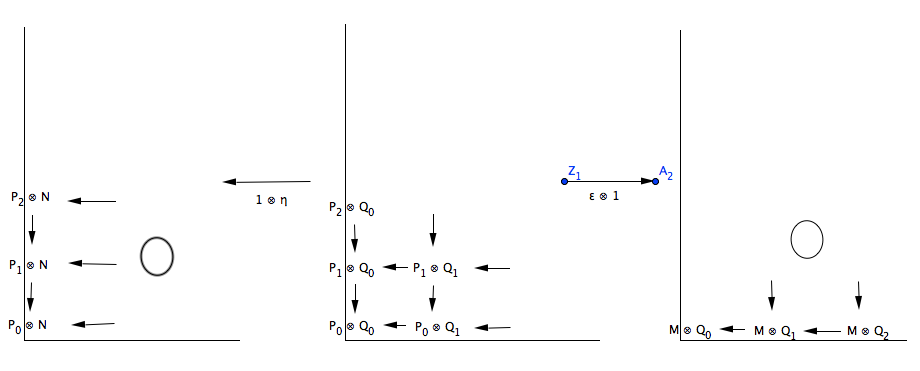
\includegraphics[width=4in]{images/bicom.png} 
\end{figure}

We want to show that $\tot(1 \otimes \eta)$ is a quasi-isomorphism, likewise for $\tot(\ep \otimes 1)$. However, the latter follows mutatis mutandis. By Lemma \ref{lemone}, it is enough to show that $1 \otimes \eta$ is a quasi-isomorphism on each row. By Lemma \ref{lemthree}, it will follow since each $P_n$ is projective, hence flat. So $P_n \otimes -$ is an exact functor so it preserves quasi-isomorphisms (show this). \qed \\

\begin{lem} \label{lemone} 
If $A_{\cdot \cdot} \ma{f} B_{\cdot \cdot}$ is a map of first quadrant bicomplexes (with arrows towards the origin or away from the origin) such that the map on each row/column is a quasi-isomorphism, then $\tot(A_{\cdot \cdot} \ma{\tot(f)} \tot(B_{\cdot \cdot})$ is a quasi-isomorphism. 
\end{lem}

\noindent Proof (Sketch): By taking cones of $f$ on the rows, one obtains a bicomplex, say $C_{\text{row/col}}(f)$. Note, $f$ is a quasi-isomorphism on the rows so that $C_{\text{row/col}}(f)$ is exact in each row/column. Also,
\[
0 \ma{} B_{\cdot \cdot} \stackrel{i}{\hra} C_{\text{row/col}}(f) \ma{\pi} A_{\cdot \cdot}[-1] \ma{} 0
\]
is exact. Then
\[
0 \ma{} \tot(B) \ma{} \tot(C_{\text{row/col}}) \ma{} \tot(A_{\cdot \cdot})[-1] \ma{} 0
\]
is exact. But the middle term is precisely $C(\tot(f))$. By Lemma \ref{lemtwo}, the sequence is exact so $\tot(f)$ is a quasi-isomorphism. \qed \\

\begin{lem} \label{lemtwo}
If $\dt{C}$ is a first quadrant bicomplex with exact rows (or columns) then $\tot(C_{\cdot \cdot})$ is exact. 
\end{lem}

\noindent Proof:
\begin{figure}[h] 
   \centering
   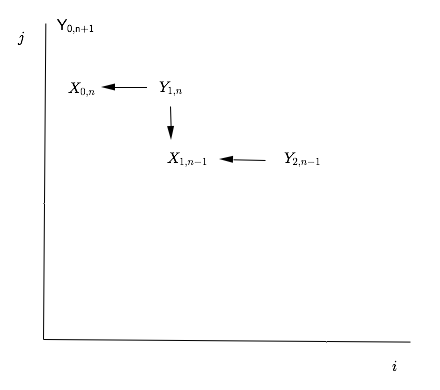
\includegraphics[width=3in]{images/arrows.png} 
\end{figure}
Let $X=(X_{ij}) \in \oplus_{i+j=n} C_{ij}$ be a cycle in $\tot(C)$, i.e. for each $i$, $(-1)^id(X_{i,n-i})+d'(X_{i-1,n-(i-1)})=0$, where $(-1)^id$ are the downwards maps in the complex and $d'$ are the left arrows in the complex. Start at the upper left. Let $Y_{0,n+1}=0$. Since $d'(X_{0,n})=0$ and the rows are exact, there is a $Y_{1,n}$ such that $d'(Y_{1,n})=X_{0,n}$. Check that $X_{1,n-1}-(-d(Y_{1,n})) \in \ker d'$. Since the rows are exact, there is a $Y_{2,n-1} \in d'(Y_{2,n-1})=X_{1,n-1}+d(Y_{1,n})$. Then ``$d$" of the $Y$'s so far are $X_{1,n-1}$. Continue this process by induction. This induction must end as the complex is 1st quadrant (at the most when it hits the axis). So ``$d$" of the $Y$'s is $(X_{ij})_{i+j=n}$, so $(X_{ij})$ is a boundary. \qed \\

\begin{lem} \label{lemthree}
Let $\dt{A} \ma{f} \dt{B}$ be a chain map (map of complexes). If $f$ is a quasi-isomorphism and $P$ is flat, then $P \otimes \dt{A} \ma{1 \otimes f} P \otimes \dt{B}$ is a quasi-isomorphism. 
\end{lem}

\noindent Proof: Suppose that $A \ma{f} B$ is a quasi-isomorphism. Then $C(f)$ is exact so that as $P$ is flat, $P \otimes \dt{C(f)}$ is exact. But this is isomorphic to $C(1 \otimes f)$. Then $1 \otimes f$ is a quasi-isomorphism. \qed \\

The same proof works for $F(-)$ instead of $P \otimes -$ if $F$ is an exact functor. Suppose
\[
0 \ma{} A \ma{} B \ma{} C \ma{} 0
\]
is an exact sequence. Then we get the exact sequence
\[
A \otimes N \ma{} B \otimes N \ma{} C \otimes N \ma{} 0
\]
We get a similar sequence for $M \otimes -$. 

\begin{cor}
We have two long exact sequences for
\[
\tor(M,N)=H_n(\dt{P} \otimes N) = H_n(M \otimes \dt{Q})
\]
\end{cor}

\subsection{Right Derived Functors}

\begin{dfn}
Let $F: \cA \to \cB$ be a left exact functor, where $\cA$ and $\cB$ are abelian and $F$ is additive. If $\cA$ has injective resolutions, then we can define a right derived functor by taking $N \in \cA$ and take injective resolution $N \to I^{\cdot}$:
\[
R^nF(N) \defeq H^n(F(I^{\cdot}))
\]
\end{dfn}

This is the same construction as before applied to $F^{\text{op}}: \cA^{\text{op}} \to B^{\text{op}}$. That is, $F$ is left exact if and only if $F^{\text{op}}$ is right exact. Similarly, we have injective resolutions in $\cA$ if and only if we have projective resolutions in $A^\text{op}$. So we have an automatic proof of:

\begin{thm}
\begin{enumerate}[(i)]
\item $R^nF: \cA \to \cB$ is well-defined (independent of the choice of injective resolution) and is a functor for all $n$
\item $R^0F=F$
\item if $0 \to A \to B \to C \to 0$ is exact, then there are a functorial, i.e. natural, maps $\delta^n$ such that we get a long exact sequence
\[
0 \ma{} R^0F(A) \ma{} R^0F(B) \ma{} R^0F(C) \ma{\delta} R^1F(A) \ma{} R^1F(B) \ma{} R^1F(C) \ma{\delta} \cdots
\]
\end{enumerate}
\end{thm}

The major example will be the Ext functor. Let $M,N \in R-\text{mod}$. Let $F(-)\defeq \Hom_R(M,-)$. Then $F$ is covariant and left exact. These right derived functors are called the Ext functors.
\[
\Ext_R^n(M,N)=R^nF(N)
\]
i.e. $H^n(\Hom(M,\dt{I}))$. 

\begin{ex}
$\Ext_{\Z}^n(\Z/k\Z,\Z)$ for $k \geq 2$. Recall over a PID, injective is equivalent to divisible. So we have an injective resolution of $\Z$
\[
0 \ma{} \Z \hra \Q \ma{} \Q/\Z \ma{} 0
\]
where $I^0=\Q$ and $I^1=\Q/\Z$, which are divisible so they are injective $\Z$-modules. Then we have
\[
0 \ma{} \Hom_{\Z}(\Z/k\Z,\Q)=0 \ma{} \Hom_{\Z}(\Z/k\Z,\Q/\Z) \ma{} 0
\]
So then we have
\[
\begin{split}
\Ext^0_{\Z}(\Z/k\Z,\Z) &= H^0(\text{above})=0/0=0 \\
\Ext^1_{\Z}(\Z/k\Z,\Z) &= H^1(\text{above})=\Hom_{\Z}(\Z/k\Z,\Q/\Z)/0
\end{split}
\]
where the maps in $\Ext_{\Z}^1$ are given by $\overline{1} \mapsto p/q$ with $(p,q)=1$ such that $k \overline{p/q}=0 \in \Z$ so that $q \mid k$ which is $\{p/q \in \Q/\Z \;|\; kp/q \in \Z\}$. 
\end{ex}

Note that $\Ext_R^0(M,N)=\Hom_R(M,N)$.

\subsection{Contravariant Functors}

If $F: \cA \to \cB$ is contravariant and left exact. We get $F^1: \cA^{\text{op}} \to \cB$ is contravariant. So this is still left exact so we can use the construction from before. So $F'$ has right derived functors which are 
\[
R^nF'(M) \defeq H^n(F'(\text{injective resolution of }M \text{ in }\cA))
\]
which is $H^n(F(\text{projective resolution of }M\text{ in }\cA))=R^nF(M)$. 

\begin{ex}
$F(-)=\Hom_R(-,N)$ is left exact. This gives $R^nF(M)=H^n(\Hom(\dt{P},N))$, where $\dt{P}$ is a projective resolution of $M$. 
\end{ex}

\subsection{Balancing Ext}

We have two derived functors to associate to $M,N \to \Hom_R(M,N)$. Namely, $\Hom(M,-)$ and $\Hom_R(-,N)$. 

\begin{thm}
If $N \ma{\eta} I^{\cdot}$ is an injective resolution and $\dt{O} \ma{\ep} M$ is a projective resolution
\[
\Ext_R^0(M,N)=H_n(\Hom(M,I^{\cdot})) \cong H_n(\tot(\Hom(\dt{P},I^{\cdot}))) \cong H_n(\Hom(\dt{P},N))
\]
\end{thm}

\begin{ex}
We redo the example from before. Take $\Ext_{\Z}^n(\Z/k\Z,\Z)$. So instead of taking a projective resolution of $\Z/k\Z$, we take a projective resolution of $\Z/k\Z$
\[
0 \ma{} \Z \ma{k} \Z \ma{} \Z/k\Z \ma{} 0
\]
where $P_1=\Z$ and $P_0=\Z$. Then we have $\Ext^n=H^n(\Hom_{\Z}(\dt{P},\Z))$ so we have
\[
0 \ma{} \Hom_{\Z}(\Z,\Z) \ma{k^*} \Hom_{\Z}(\Z,\Z) \ma{} 0 
\]
which is
\[
0 \ma{} \Z \ma{k} \Z \ma{} 0
\]
So that $\Ext_{\Z}^0(\Z/k\Z,\Z)=0$ and $\Ext_{\Z}^1(\Z/k\Z,\Z)=\Z/k\Z$, which is the subgroup $\langle 1/k \rangle$ of $\Q/\Z$. 
\end{ex}

\begin{cor}
If 
\[
0 \ma{} A \ma{} B \ma{} C \ma{} 0
\]
is exact. There are two types of long exact sequences
\[
0 \to \Hom(M,A) \to \Hom(M,B) \to \Hom(M,C) \ma{\delta} \Ext^1(M,A) \to \Ext^1(M,B) \to \Ext^1(M,C) \ma{\delta} \cdots
\]
and the long exact sequence
\[
0 \to \Hom(C,M) \to \Hom(B,M) \to \Hom(A,M) \ma{\delta} \Ext^1(C,M) \to \Ext^1(C,M) \to \Ext^1(A,M) \ma{\delta} \cdots
\]
\end{cor}

Note that since $\Tor$ and $\Ext$ are balanced, there is another way to get the same long exact sequence (avoiding the Horseshoe Lemma). For example for $\Ext$, if we have the exact sequence
\[
0 \ma{} A \ma{} B \ma{} C \ma{} 0
\]
and an $R$-module $M$, we take a projective resolution $\dt{P} \to M$ of $M$, then
\[
0 \to \Hom(\dt{P},A) \to \Hom(\dt{P},B) \to \Hom(\dt{P},C) \to 0
\]
is an exact sequence of complexes since each $P_n$ is projective (hence preserving exactness). Taking the long exact sequence on homology.

Note also that if $R$ is commutative with $M,N$ being $R$-modules, if $M \ma{r} N$ is multiplication by $r$, then the induced maps on $M \otimes N$, $\Hom(M,N)$, and $\Hom(N,M)$ are just multiplication by $r$. So too are the maps on $\Tor(N,M),\Tor(M,N),\Ext^n(M,n)$, and $\Ext^n(M,N)$. 

\begin{cor}[Tor Balanced]
We have
\[
\Tor_n^R(M,N) \cong \Tor_n^{R^{\text{op}}}(N,M)
\]
\end{cor}

\noindent Proof (Sketch): This is simple as $M \otimes_R N \cong N \otimes_{R^{\text{op}}} M$, which is easily demonstrated. \qed \\

\begin{cor}
The following are equivalent for an $R$-module $F$:
\begin{enumerate}[(i)]
\item $F$ is flat; that is, $F \otimes_R -$ is exact.
\item $\Tor_n^R(F,N)=0$ for all $n>0$.
\item $\Tor_1(F,N)=0$
\end{enumerate}
\end{cor}

\noindent Proof:
\begin{enumerate}
\item[(i)$\to$(ii):] Suppose that $F$ is flat. Take a projective resolution $\dt{P} \to N$ of $N$, then we have
\[
\Tor_n^R(F,N) \defeq H_n(F \otimes_R \dt{P})= F \otimes_R H_n(\dt{P})=0
\]
since $F\otimes_R -$ is an exact functor. 

\item[(ii)$\to$(ii):] This is obvious.

\item[(iii)$\to$(i):] Start with an exact sequence
\[
0 \ma{} A \ma{} B \ma{} C \ma{} 0
\]
Tensoring with $F$ preserves right exactness
\[
\Tor_1(F,C)=0 \ma{} F \otimes_R A \ma{} F \otimes_R B \ma{} F \otimes_R C \ma{} 0
\]
as $\Tor_1(F,C)=0$ by assumption. 
\end{enumerate}
\qed \\

\begin{cor}
One can use flat resolutions instead of projective resolutions to compute $\Tor$.
\end{cor}

\noindent Proof: This follows easily by the proceeding corollary and dimension shifting. One can also easily show this using the fact that $\Tor$ is balanced. \qed \\

\begin{prop}
The following are equivalent for an $R$-module $P$:
\begin{enumerate}[(i)]
\item $P$ is projective
\item $\Ext^n_R(P,-)=0$ for $n>0$
\item $\Ext_R^1(P,-)=0$
\end{enumerate}
\end{prop}

\noindent Proof: This is left as an exercise but it follow quickly using the fact that $\Hom(P,-)$ is exact. \qed \\

\begin{prop}
The following are equivalent for any $R$-module $I$:
\begin{enumerate}[(i)]
\item $I$ is injective
\item $\Ext_R^n(-,I)=0$ for all $n>0$
\item $\Ext_R^1(-,I)=0$
\end{enumerate}
\end{prop}

\noindent Proof: L.T.R. \qed \\

\begin{prop}[Localization]
Let $R$ be a commutative ring and $S$ be a multiplicatively closed subset of $R$.
\begin{enumerate}[(i)]
\item $S^{-1}\Tor_n^R(M,N) \cong \Tor_n^{S-R}(S^{-1}M,S^{-1}N)$
\item If $M$ is finitely presented, we have $\Ext_R^n(M,N) \cong \Ext_R^{S-R}(S^{-1}M,S^{-1}N)$.
\end{enumerate}
\end{prop}

\subsection{K\"unneth Formula and the Universal Coefficient Theorem}

\begin{thm}[K\"unneth Formula]
Let $\dt{P}$ be a chain complex of right $R$-modules such that 
\begin{enumerate}[(i)]
\item each $P_n$ is flat
\item each $B_{n-1}=d(P_n)$ is flat
\end{enumerate}
then for each $n$ and each left $R$-module $M$, there is an exact sequence
\[
0 \ma{} H_n(\dt{P}) \otimes M \ma{} H_n(\dt{P} \otimes M) \ma{} \Tor_1^R(H_{n-1}(P),M) \ma{} 0
\]
\end{thm}

\noindent Proof: Consider the short exact sequence
\[
0 \ma{} Z_n \hra P_n \ma{d_n} B_{n-1} \ma{} 0
\]
where $P_n,B_{n-1}$ are flat. By the long exact sequence for $\Tor$ along with the fact that $P_n$ and $B_{n-1}$ are flat, we know that $Z_n$ are flat. Tensoring with $M$ yields
\[
\cdots \to 0=\Tor_1(B_{n-1},M) \to Z_n \otimes M \to P_n \otimes M \to B_{n-1} \otimes M \to 0
\]
where the left is 0 as $B_{n-1}$ is flat. Then we have
\[
0 \ma{} Z_n \otimes M \ma{} P_n \otimes M \ma{} B_{n-1} \otimes M \ma{} 0
\] 
Putting these together for all $n$, we get a short exact sequence of complexes
\[
0 \ma{} \dt{Z} \otimes M \ma{} \dt{P} \otimes M \ma{d \otimes 1} (\dt{B} \otimes M)[-1] \ma{} 0
\]
with differentials on $Z$ and $B$ inherited from $d$ on $\dt{P}$, so 0. That is, $d^Z=0$ and $d^B=0$. Then the long exact sequence on homology is
\[
\begin{split}
\cdots \ma{} H_{n+1}((B \otimes M)[-1]) &\ma{\delta} H_n(Z \otimes M)=Z_n \otimes M \ma{} H_n(P \otimes M) \ma{} \\
&H_n((B \otimes M)[-1]) \ma{\delta} H_{n-1}(Z \otimes M) \ma{} \cdots
\end{split}
\]
We have $Z_n \otimes M/(i \otimes 1)(B_n \otimes M)= Z_n/B_n \otimes M$. But $H_n(\dt{P})=Z_n/B_n$. Since $\otimes$ is right exact, we have
\[
0 \ma{} B_{n-1} \ma{} Z_{n-1} \ma{} H_{n-1} \ma{} 0
\]
This is a flat resolution of $H_{n-1}(P)$. So $\ker \delta=\ker(i \otimes 1)=\Tor_1(H_{n-1}(P),M)$ by the resolution above. \qed \\

Note that the term of the K\"unneth Formula is the middle term. However, when does this even hold? Particularly, when does (ii) hold? The major case when $\dt{P}$ is projective (a fortiori flat) and $R$ is hereditary. 

\begin{dfn}[Hereditary Ring]
We call $R$ a hereditary ring if submodules of projective modules are projective. Equivalently, every module has projective dimension at most 1.
\end{dfn}

\begin{ex}
Some easy examples of hereditary rings are $R=\Z$, PIDs, and Dedekind domains.
\end{ex}

In fact, we get a stronger result.
\begin{thm}[Universal Coefficient Theorem]
Let $\dt{P}$ be a chain complex of right $R$-modules such that
\begin{enumerate}[(i)]
\item each $P_n$ are projective
\item each $B_{n-1}=d(P_n)$
\end{enumerate}
then the K\"unneth Formula holds and the sequence (non-canonically) splits. 
\[
H_n(\dt{P} \otimes M) \cong (H_n(\dt{P}) \otimes M) \oplus \Tor_1^R(H_{n-1}(\dt{P}),M)
\]
\end{thm}

We also have similar formulas for complexes:

\begin{thm}[K\"unneth Formula for Complexes]
If $\dt{P},\dt{Q}$ are complexes of left/right $R$-modules with each $P_n$ flat and each $B_{n-1}=d(P_n)$ flat, then for all $n$ there is an exact sequence
\[
0 \ma{} \oplus_{p+q=n} H_n(P) \otimes H_q(Q) \ma{} H_n(\tot(\dt{P} \otimes \dt{Q})) \ma{} \oplus_{p+q=n-1} \tor_1^R(H_p(P), H_q(Q)) \ma{} 0
\]
If each $P_n,B_{n-1}$ are projective, then this sequence splits.
\end{thm}

Notice this result is useful for products of spaces!

\begin{thm}[Universal Coefficient Theorem for Cohomology]
Let $M$ be a left $R$-module and $\dt{P}$ be a chain complex such that 
\begin{enumerate}[(i)]
\item each $P_n$ is projective
\item each $B_{n-1}=d(P_n)$ are projective
\end{enumerate}
then for all $n$ we have a (non-canonically) split exact sequence
\[
0 \ma{} \Ext_R^1(H_{n-1}(P),M) \ma{} H^n(\Hom(\dt{P},M)) \ma{} \Hom(H_n(\dt{P},M)) \ma{} 0
\]
\end{thm}

\subsection{Tor}

Historically, Tor is related to
\begin{enumerate}[(i)]
\item to torsion (see 7.13 of Rotman's \emph{Introduction to Homological Algebra})
\item Serre used Tor to give an algebraic foundation for intersection multiplicity:
\[
\chi(R/I,R/J)\defeq \sum_{i=0}^d (-1)^il(\Tor_i^R(R/I,R/J))
\]
for varieties $V(I),V(J)$ is a smooth space given by $R$, $\spec R$. 
\end{enumerate}

\subsection{Ext and Extensions}

For this section, we will be in $R$-mod. 

\begin{dfn}[Extension]
An extension of $C$ by $A$ is an exact sequence
\[
\xi: 0 \ma{} A \ma{i} X \ma{} C \ma{} 0
\]
Note that $C \cong X/i(A)$ and $A \cong i(A)/0$. Two extensions $\xi,\xi'$ are equivalent if there exists a map $\varphi$ such that we have the commutative diagram
\[
\begin{tikzcd}
\xi: & 0 \arrow{r} A \arrow{d}{=} \arrow{r} & X \arrow{d}{\varphi} \arrow{r} & C \arrow{d}{=} \arrow{r} & 0 \\
\xi': & 0 \arrow{r} & A \arrow{r} & X' \arrow{r} & C \arrow{r} & 0 
\end{tikzcd}
\]
Observe by the Five-Lemma (or the Snake Lemma), $\varphi$ is an isomorphism. We denote the equivalence class of $\xi$ by $[\xi]$. 
\end{dfn}

\begin{rem}
Any split extension is equivalent to the trivial one:
\[
0 \ma{} A \stackrel{i}{\hra} A \oplus C \ma{\pi_2} C \ma{} 0
\]
\end{rem}

\begin{dfn}[$e(C,A)$]
For the moment, we define $e(C,A)$ as the set of equivalence classes $[\xi]$.
\end{dfn}

\begin{thm}
There is a bijection $e(C,A) \ma{\theta} \Ext_R^1(C,A)$, $\Ext_R^1(C,A) \ma{\psi} e(C,A)$ in which the split extension corresponds to $0 \in \Ext_R^1(C,A)$.
\end{thm}

\noindent Proof: Choose a projection $\dt{P} \to C$. Recall to compute $\Ext_R^1(C,A)=H^1(\Hom(\dt{P},A))=H^1(0 \to \Hom(P_0,A) \ma{d_1^*} \Hom(P_1,A) \ma{d_2^*} \Hom(P_2,A) \ma{} \cdots)$. By the Comparison Theorem, $1_C$ lifts to a chain map
\[
\begin{tikzcd}
\cdots \arrow{r} & P_2 \arrow[dotted]{d}{0} \arrow{r}{d_2} & P_1 \arrow[dotted]{d}{\alpha_1} \arrow{r} & P_0 \arrow[dotted]{d}{\alpha_0} \arrow{r} & C \arrow{d}{=} \arrow{r} & 0 \\
\cdots \arrow{r} & 0 \arrow{r} & A \arrow{r} & X \arrow{r} & C \arrow{r} & 0
\end{tikzcd}
\]
Commutativity gives $d_2^*(\alpha_1)=\alpha_1d_2=0$. So $\alpha_1$ is a cycle. To define $\theta$, given an extension 
\[
\xi: 0 \ma{} A \ma{i} X \ma{} C \ma{} 0
\]
let $\theta(\xi) \defeq \overline{\alpha}_1 \in \ker d_2^*/\im d_1^*$. Note that this is well defined as given another lift of $1_C$, say $\alpha' \simeq \alpha$, so there is a $s$ such that $\alpha_1-\alpha'=0s_1+s_0d_1=s_0d_1 \in \im d_1^*$. So $\alpha_1=\alpha' \in \Ext_R^1(C,A)$. Furthermore, if $[\xi]=[\xi']$, one gets the commutative diagram
\[
\begin{tikzcd}
\cdots \arrow{r} & P_2 \arrow[dotted]{d}{\alpha_2} \arrow{r} & P_1 \arrow[dotted]{d}{\alpha_1} \arrow{r} & P_0 \arrow[dotted]{d}{\alpha_0} \arrow{r} & C \arrow{d}{=} \arrow{r} & 0 \\
\cdots \arrow{r} & 0 \arrow{r} & A \arrow{d}{=} \arrow{r} & X \arrow{d}{\varphi} \arrow{r} & C \arrow{d}{=} \arrow{r} & 0 \\
\cdots \arrow{r} & 0 \arrow{r} & A \arrow{r} & X' \arrow{r} & 0 \arrow{r} & 0
\end{tikzcd}
\]
$\varphi\alpha_1$ is the vertical composition for the lift for $\xi'$ So $\theta([\xi']) \defeq 1_A \alpha_1$ and $\theta([\xi])\defeq \alpha_1$, which are equal. Finally, $\theta$ takes trivial split extensions to 0 as
\[
\begin{tikzcd}
\cdots \arrow{r} & P_2 \arrow{dl} \arrow{r} & P_1 \arrow{dl}{\alpha_1=0} \arrow{r} & P_0 \arrow{dl}{(0 \; \ep)^T} \arrow{r} & C \arrow{r} \arrow{d}{=} & 0 \\
\cdots \arrow{r} & 0 \arrow{r} & A \arrow{r} & A \oplus C \arrow{r}{\pi_2} C \arrow{r} & 0
\end{tikzcd}
\]
so that $\theta([\xi])=\overline{\alpha}_1=0$. 

We now need to define $\psi$. Given an element $\overline{\beta} \in \Ext_R^1(C,A)$, we have $\beta: P_1 \to A \in \Hom(P_1,A)$ such that $\beta$ is a cycle, i.e. $d_2^*(\beta)=0$ so that $\beta d_2=0$. So we have 
\[
\begin{tikzcd}
\cdots \arrow{r} & P_2 \arrow{r}{d_2} & P_1 \arrow{d}{\beta} \arrow{r}{d_1} & P_0 \arrow{r}{\ep} & C \arrow{d}{=} \arrow{r} & 0 \\
\cdots \arrow{r} & 0 \arrow{r} & A \arrow{r}{i} & ? \arrow{r}{p} & C \arrow{r} & 0 
\end{tikzcd}
\]
Let $X$ be the pushout
\[
\begin{tikzcd}
P_1 \arrow{d}{\beta} \arrow{r}{d_1} & P_0 \arrow{d}{\beta_0} \\
A \arrow{r}{i} & X
\end{tikzcd}
\]
For an abelian category, $X \in (A \oplus P_0)/L$, where $L=\{(\beta(x),-d_1(x))\}$. Let $p: A \oplus P_0 \to C$ be given by $(a,p) \mapsto \ep(p)$. Since $L \subseteq \ker p$, we get an induced map $(A \oplus P_0)/L=X \ma{p} C$. Putting all this in the diagram, it is routine to verify that it commutes. 
\[
\begin{tikzcd}
\cdots \arrow{r} & P_1 \arrow{d}{\beta} \arrow{r} & P_0 \arrow{d}{\beta_0} \arrow{r} & C \arrow{d}{=} \arrow{r} & 0 \\
\cdots \arrow{r} & 0 \arrow{r} & A \arrow{r} & X \arrow{r}{p} & C \arrow{r} & 0
\end{tikzcd}
\]
Moreover, the bottom row is exact. Define $\psi(\overline{\beta})$ to be the bottom row of the extension. It is simple enough to show that this is well defined (if $\beta=\beta'+d_1^*(J)$ for some $J$, we get isomorphic pushouts, possibly modifying $\beta_0$ to $\beta_0+Ji$). 

It is simple to see that $\theta \psi=1$ (we used $\beta$ to construct the pushout so we clearly get $\beta$ back under $\theta$). To see $\psi \theta=1$, show that $X$ is the pushout of the given $\alpha_1$ and $d_1$. \qed \\

\begin{cor}
$\Ext_R^1(C,A)=0$ if and only if every extension of $C$ by $A$ splits.
\end{cor}

Now under this bijection, we see that these are the same as sets. But are they the same as groups? We know that $\Ext$ has an abelian structure. Does $e(C,A)$ have an abelian structure? We want to set a group structure on $e(C,A)$ ``agreeing" with $\theta$. 

\subsection{Baer Sum (1934)}

Lets define addition on $e(C,A)$. If $\xi: 0 \ma{} A \ma{i} X \ma{p} C \ma{} 0$ and $\xi': 0 \ma{} A \ma{i'} X \ma{p'} C \ma{} 0$ are extensions of $C$ by $A$, let $X''$ be the pullback of $p,p'$
\[
\begin{tikzcd}
X'' \arrow{r} \arrow{d} & X' \arrow{d} \\
X \arrow{r} & C
\end{tikzcd}
\]
so $X''=\{(x,x') \in X \times X' \;|\; p(x)=p'(x') \text{ in }C\}$. We hope for a kernel but $A$ is too ``big". Let $Y=X''/\{(-i(a),i'(a))\}_{a \in A}$, i.e. we identify two copies of $A$ in $X \times X'$. Then 
\[
0 \ma{} A \ma{} Y \ma{} C \ma{} 0
\]
with maps $a \mapsto (i(a),0)=(0,i(a))$ and $(x,x') \mapsto p(x)$. Note that $p(x)=p'(x)$ is exact (one should verify this). This extension is called the Baer Sum: $\xi+\xi'$. 

\begin{thm}
The Baer sum in $e(C,A)$ agrees under $\theta$ with the usual $+$ in $\Ext_R^1(C,A)$, i.e. $\theta(\xi+\xi')=\theta(\xi)+\theta(\xi')$. Hence, the sum is well defined on equivalence classes $[\xi]$ and under the Baer sum $e(C,A)$ is a group. 
\end{thm}

\noindent Proof: This is far too long to present here. \qed \\

\subsection{Yoneda Extension}

Similarly, 
\begin{thm}
We have an isomorphism (as sets and groups)
\[
\Ext_R^n(C,A) \cong \{\text{Extensions } \xi: 0 \ma{} A \ma{} X_n \ma{} \cdots \ma{} X_1 \ma{} C \ma{} 0\}/ \sim
\]
where $\sim$ is the equivalence relation $\xi \sim \xi'$ if there are $\alpha$'s such that 
\[
\begin{tikzcd}
\xi: & 0 \arrow{r} & A \arrow{d}{=} \arrow{r} & X_n \arrow{r} \arrow{d}{\alpha_n} & \cdots \arrow{r} & X_1 \arrow{d}{\alpha_1} \arrow{r} & C \arrow{d}{=} \arrow{r} & 0 \\
\xi': & 0 \arrow{r} & A \arrow{r} & X_n' \arrow{r} & \cdots \arrow{r} & X_1' \arrow{r} & C \arrow{r} & 0 
\end{tikzcd}
\]
commutes. The group structure is addition of extensions $\xi+\xi' \defeq$ the extension
\[
0 \ma{} A \ma{} Y_n \ma{} X_{n-1} \oplus X'_{n-1} \ma{} \cdots \ma{} X_2 \oplus X_2' \ma{} X_1 '' \ma{} C \ma{} 0
\]
where $Y_n,X_1''$ are the constructed pieces
\[
\begin{split}
X_1''&= \text{ pullback } X_1,X_1' \text{ over }C? \\
Y_n &= \text{ pushout } X_1,X_1'' \text{ over }A?
\end{split}
\]

\end{thm}



































\newpage
% !TEX root = ../../homo_alg.tex

\newpage
\section{The Derived Category}

\subsection{Derived Categories \& Localization of Categories}

To get better behavior (in the same way that the long exact sequence corrected non exactness), we want to replace modules $M$ by their projective resolutions $\dt{P}$. Note $\dt{P}$ is quasi-isomorphic to $M$. We naturally come to a category where quasi-isomorphic objects are somehow the same, i.e. quasi-isomorphisms are considered isomorphisms. 

Let $\cA$ be an abelian category. Let $\chh(\cA)$ be the (abelian) category of cochain complexes. 

\begin{dfn}[Derived Category]
The derived category $\cD(\cA)$ is a category equipped with a functor $\chh(\cA) \ma{i} \cD(\cA)$ with $i(f)$ an isomorphism for all quasi-isomorphisms $f$ satisfying the universal mapping property: any functor $\chh(\cA) \ma{F} \cC$ transforming quasi-isomorphisms factors uniquely through $\cD(\cA)$. That is, we have a unique $G$ such that the following diagram commutes:
\[
\begin{tikzcd}
\chh(\cA) \arrow{r}{F} \arrow{dr}{i} & \cC \\
& \cD(\cA) \arrow{u}{G}
\end{tikzcd}
\]
Note if such a category exists, it is unique up to isomorphism. 
\end{dfn}

We show the existence of such a category by physically constructing $\cD(\cA)$ by inverting all quasi-isomorphisms. Namely, we will ``localize" $\chh(\cA)$. One should read Gelfand-Manin chapters 3 and 4 for more on this material generally. 

In the proceeding lemma, the category $\cB=\chh(\cA)$ and $S=\{\text{quasi-iso in }\chh(\cA) \subseteq \text{morph }\chh(\cA)\}$. We want to show $\cD(\cA)= S^{-1}\cB$. 

\subsection{Localization of a Category}

Let $\cB$ be a category and let $S$ be a collection of morphisms. Define $S^{-1}\cB$ by $\ob(S^{-1}\cB)\defeq \ob(\cB)$ and morphisms by for each $X \ma{s} Y$ in $S$, adjoin a ``morphism" $X \xleftarrow{s^{-1}} Y$ in $S^{-1}\cB$. Note that $s^{-1}$ is not a morphism in $\cB$ but rather a symbol of sorts. The morphisms in $S^{-1}\cB$ are formal products of morphisms in $\cB$ and these formal inverses $S^{-1}$ for $s \in S$ such that the ``codomain" of each is the ``domain" of the next modulo an equivalence generated by 
\begin{enumerate}[(i)]
\item consecutive morphisms in $\cB$ can be replaced by compositions in $\cB$. 
\item $ss^{-1} \notin S^{-1}S$ can be replaced by $1$.
\item $1s^{-1}=s^{-1}=s^{-1}1$.
\end{enumerate}

so that composition is just concatenation. 

\begin{prop}
\begin{enumerate}[(i)]
\item $S^{-1}\cB$ is a category
\item $i: \cB \to S^{-1}\cB$ given on objects by $\ob: X \mapsto X$ and on morphisms by $f \mapsto f$ is a functor.
\item The category satisfies the universal mapping property for all functors $\cB \ma{F} \cC$ transforming morphisms in $S$ into isomorphism in $\cC$. That is, there is a unique functor $G$ such that 
\[
\begin{tikzcd}
\cB \arrow{r}{F} \arrow{dr}{i} & \cC \\
&  S^{-1}\cB \arrow[dotted]{u}{G}
\end{tikzcd}
\]
\end{enumerate}
\end{prop}

\noindent Proof: The proof of the first two parts is dull and routine verification. For the third, on objects let $G(X)=F(X)$ of $S^{-1}\cB$. Let $G(s_1^{-1}f_1s_2^{-1}f_2 \cdots)=F(s_1)^{-1}F(f_1)F(s_2)^{-1}F(f_2) \cdots$. Note that $i(s)$ in $S^{-1}\cB$ is invertible, $i(s)=s$ so $ss^{-1}=1$ and $s^{-1}s=1$. \qed \\

So we have $\cD(\cA)=S^{-1}(\chh(\cA))$, where $S=\{\text{quasi-iso}\}$. We have a similar description of $S^{-1}\cB$ when $S$ is localizing. 

\begin{dfn}[Localizing Morphisms]
A collection $S \subseteq \text{morph of }\cB$ is localizing if
\begin{enumerate}[(a)]
\item all $1_X \in S$ and $s,t \in S$ implies $st \in S$.
\item for all $f \in S$ with $s \in S$ with the same codomain, there exist $g,t$ with $t \in S$ with a $W$ such that the following square commutes
\[
\begin{tikzcd}
W \arrow{d}{\ep} \arrow{r}{g} & Z \arrow{d}{s} \\
X \arrow{r}{f} & Y 
\end{tikzcd}
\]
\item for $g,t$ as given above, there exist $s,f$ as above.
\item For any $f,g$, there exist $s \in S$ such that $sf=sg$ if and only if there is a $t \in S$ such that $ft=gt$.

\begin{figure}[H] 
   \centering
   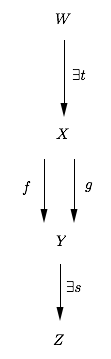
\includegraphics[width=0.5in]{images/p1.png} 
\end{figure}

\end{enumerate}
\end{dfn}

Note the second condition above gives for all $f,s$, there is a $g,t$ such that $ft=sg$ so that in $S^{-1}\cB$, $s^{-1}f=gt^{-1}$ so we can ``rearrange" until all $s$'s (denominators) are on the right and all the $f$'s (numerators) are on the left.

\begin{prop}
Let $S$ be a localizing collection of morphisms. Then $S^{-1}\cB$ can be defined equivalently as 
\begin{enumerate}[(a)]
\item $\ob(S^{-1}\cB)=\ob(\cB)$
\item morphisms $X \to Y$ in $S^{-1}\cB$ are equivalence classes of ``roofs" 

\begin{figure}[H] 
   \centering
   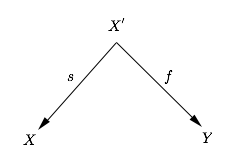
\includegraphics[width=2.5in]{images/p2.png} 
\end{figure}

with $s \in S$, written $(s,f)$. This corresponds to $fs^{-1}$ from the ``old" description of $S^{-1}\cB$. That is, $(s,f) \sim (t,g)$ if and only if there is a commutative diagram


\begin{figure}[H] 
   \centering
   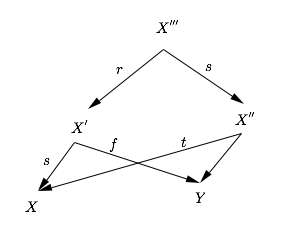
\includegraphics[width=2.5in]{images/p3.png} 
\end{figure}

with $sr \in S$ (but not necessarily $r \in S$). Or that we have the diagram 

\begin{figure}[H] 
   \centering
   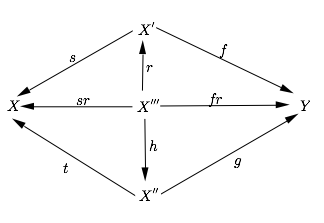
\includegraphics[width=2.5in]{images/p4.png} 
\end{figure}

\item the identity morphism on $X$ is the roof $(1_X,1_X)$.

\item composition of roofs $(s,f)$ and $(t,g)$ is $(st',gf')$ from the diagram

\begin{figure}[H] 
   \centering
   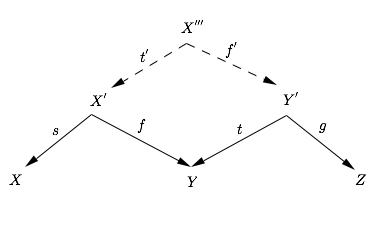
\includegraphics[width=2.5in]{images/p5.png} 
\end{figure}

where the square $f'$ and $t'$ comes from the localizing property. [$gt^{-1}fs^{-1}=gf'(t')^{-1}s^{-1}$]


\item $i: \cB \to S^{-1}\cB$ is given by on objects by $X \mapsto X$ and given on morphisms by $f \mapsto $ the roof $(1,f)$. 

\end{enumerate}
\end{prop}

\noindent Proof: We first show that $\sim$ is an equivalence relation. The reflective and symmetric properties are simple. To see the transitive property, suppose $(s,f) \sim (t,g)$ and $(t,g) \sim (u,e)$, then

\begin{figure}[H] 
   \centering
   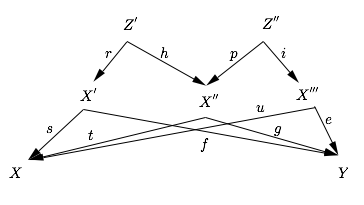
\includegraphics[width=2.5in]{images/p6.png} 
\end{figure}

so we have the commutative diagram as given above with $sr,tp \in S$. By the localizing property, there are $v,k$ with $v \in S$ such that we have

\begin{figure}[H] 
   \centering
   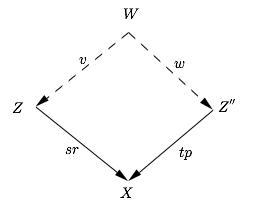
\includegraphics[width=1.5in]{images/p7.png} 
\end{figure}

Now $t=pk=srv=thv$ so there is $Z''' \ma{w} W$ is $S$ such that $pkw=hvw$ so that we have the diagram

\begin{figure}[H] 
   \centering
   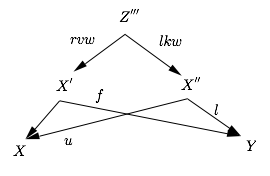
\includegraphics[width=1.5in]{images/p8.png} 
\end{figure}

commuting so $(s,f) \sim (u,e)$. So $\sim$ on roofs is an equivalence relation. Similarly, one can see that composition on roofs is well defined. Furthermore, the category with objects being the objects of $\cB$ and morphisms given by roofs is a category. We show that this category $R$ satisfies the universal mapping property for $S^{-1}\cB$ so that $R=S^{-1}\cB$. 

Given any functor $\cB \ma{F} \cC$ such that $F$ takes morphisms in $S$ to isomorphism in $\cC$, we need to show that there is a unique functor $G$ such that the following diagram commutes
\[
\begin{tikzcd}
\cB \arrow{r}{F} \arrow[hook]{dr}{i} & \cC \\
& R \arrow[dotted]{u}{G}
\end{tikzcd}
\]
where $i$ takes objects to objects via $X \mapsto X$ and on morphisms $f \mapsto (1,f)$. If $G$ exists, then it is unique as $G(X) \defeq G(i(X))=F(X)$ and 
\[
G(f)=G(i(f))=G((s,t))=G((1,s)^{-1}(1,f))=G((1,s))^{-1}G(i(f))=F(s)^{-1}F(f)
\]
Existence of such follows from the above definition. One only need show that it is indeed a functor. \qed \\

\subsection{Homotopy Category, $\cK(\cA)$}

Note that for $\cB=\chh(\cA)$ and $S=\{\text{quasi-iso}\}$, we have $\cD(\cA)\defeq S^{-1}\cB$. Unfortunately, $S$ is \emph{not} a localizing class. But it is if we go ``mod homotopy". 

\begin{dfn}[Homotopy Category]
The homotopy category $\cK(\cA)$ is the category given by $\ob(\cK(\cA))=\ob(\chh(\cA))$, that is cochain complexes, and $\text{morph}(\cK(\cA))$ is the cochain maps modulo homotopy, i.e. $\Hom_{\cK(\cA)}(X,Y)=\Hom_{\chh(\cA)}(X,Y)/\sim$, where $\sim$ is the equivalence $f \sim g$ if and only if $f \simeq g$. 
\end{dfn}

For a complex $K^\cdot$, define $K[x]$ to be $K[n]^i\defeq K^{n+1}$ and $d_{K[x]}=(-1)^n d_k$, called the shift, translation, or suspension. This gives a functor which is an equivalence of categories on $\chh(\cA),\cK(\cA),\cD(\cA)$. For any map $K^\cdot \ma{f} L^\cdot$, we have $C(f)=L^\cdot \oplus K^\cdot[1]$ with mixed differentials and $\cyl(f)=L \oplus K[1] \otimes K$ with differential from the ``tot"

\begin{figure}[H] 
   \centering
   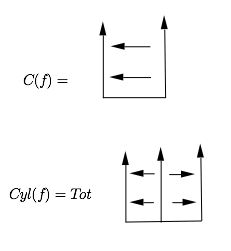
\includegraphics[width=2.5in]{images/p9.png} 
\end{figure}

\begin{lem}
For any cochian map, $K \ma{p} Y$, there is a commutative diagram with exact rows
\[
\begin{tikzcd}
0 \arrow{r} & L \arrow{d}{\alpha} \arrow{r}{i} & C(f) \arrow{r}{p} \arrow{d} & K[1] \arrow{r} & 0 \\
0 \arrow{r} & \cyl(f) \arrow{r} & C(f) \arrow{r} & ? \arrow{r} & 0
\end{tikzcd}
\]
where $\beta(l,k,k')=l+f(K)$ and other maps $\alpha,i,p,\tilde{f},\pi$ are simple inclusions/projections. Furthermore, $\alpha,\beta$ are homotopy equivalent: $\alpha \beta=1_C$ and $\beta \alpha \simeq 1_{C(y)}$ and the pictorial is functional in $f$. 
\end{lem}

\begin{lem}
Let $f,g: K \to L$ with $f \simeq g$, i.e. $f=g$ in $\cK(\cA)$. 
\end{lem}

\noindent Proof: Note that $\cyl(1_K)= \tot(K \leftarrow K \rightarrow K)$. It has two inclusions from $K$: $\alpha(k)=(k,0,0)$ with $\beta \alpha=1, \alpha\beta \simeq 1$ and $\alpha'(k)=(0,0,k)$ with $\beta\alpha'=1,\alpha'\beta\simeq 1$. 

Let $t=\alpha \beta,t'=\alpha'\beta$. Note that $t,t' \in S$ because they are homotopic to 1. Then $tt'=\alpha'\beta\alpha\beta=t'$. Then we have
\[
i(t't)=i(t')=i(t')i(t)=i(t')
\]
as they are isomorphic in $S$ so isomorphic in $\cD(\cA)$. Then we have $i(t)=1$ in $\cD(\cA)$. So
\[
i(\alpha')=i(t)i(\alpha')=i(t\alpha')=i(\alpha\beta\alpha')=i(\alpha)
\]
If $f \simeq g$ via the homotopy $\{s_n: K^{n+1} \to L^n\}$, we construct the map $\gamma=(f,s,g): \cyl(1_k) \to L$. Check that $\gamma$ is a cochain map so that it commutes with differentials (uses the fact that $s$ is a homotopy). Check also that $\gamma \alpha=f$ and $\gamma \alpha'=g$. So 
\[
i(f)=i(\gamma\alpha)=i(\gamma)i(\alpha)=i(\gamma)i(\alpha')=i(g)
\]

\begin{figure}[H] 
   \centering
   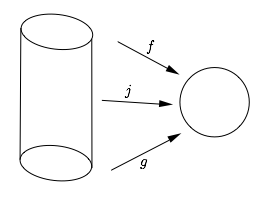
\includegraphics[width=2.5in]{images/p10.png} 
\end{figure}

So we are getting a mapping cylinder to some object so that the map of the top and bottom are the same somehow. \qed \\

\begin{thm}
\begin{enumerate}[(i)]
\item The functor 
\[
\begin{tikzcd}
i: \chh(\cA) \arrow{r} \arrow{dr}{\pi} & \cD(\cA)=S^{-1}\chh(\cA) \\
& \cK(\cA) \arrow[dotted]{u}{\exists}
\end{tikzcd}
\]
factors through $\cK(\cA)$. 

\item $\cD(\cA)=S^{-1}\cK(\cA)$ with $S=\{\text{equiv classes of quasi-iso}\}$. Note that if two morphisms are in the same equivalence class and one is a quasi-iso then the other is.

\item $S$ is a localizing class in $\cK(\cA)$. So you can describe $\cD(\cA)$ as ``roofs of maps modulo homotopy". 
\end{enumerate}
\end{thm}

\noindent Proof: The first part is obvious from the proceeding lemma. For the second part, this is easy from the universal mapping property of localization $R \to S^{-1}R$. For the third part, we need show that $S=\{\text{quasi-iso}\}$ is a localizing class in $\cK(\cA)$. Note that $1_X \in S$ and that if $f,g$ are quasi-iso then $fg$ is a quasi-iso. Then given $f,s$ with $s$ a quasi-iso, we need to find $g,t$ with $t$ quasi-iso so that 

\begin{figure}[H] 
   \centering
   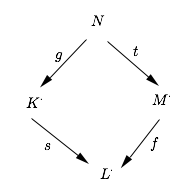
\includegraphics[width=1.5in]{images/p11.png} 
\end{figure}

Form the cone of $s$. Compose $i$ with $f$ to form the cone of $if$:
\[
\begin{tikzcd}
C(if)[-1] \arrow[dotted]{d} \arrow{r}{t} & M \arrow{d}{f} \arrow{r}{if} & C(s) \arrow{d}{=} \arrow{r} & C(if) \\
K \arrow{r}{s} & L \arrow{r}{i} & C(s) & 
\end{tikzcd}
\]
where $t$ is the usual projection to $M$ and $g$ is the usual projection to $K$. The square does not commute in $\chh(\cA)$ as $f(m) \neq s(k)$. But it is commutative up to homotopy. $ft \simeq sg$ via the homotopy $\sigma(m,l,k)=l^{n-1}$. It is routine to check that this works. Hence, the diagram commutes in $\cK(\cA)$. It is also easy to check that this is a quism and that the quism for the long exact sequence of $C(s)$ is exact so that $t$ is a queasy. Similarly, $g,t$ given as above shows there is a $f,s$ as above. For the final part, suppose 
\[
\begin{tikzcd}
K \arrow[yshift=1ex]{r}{f} \arrow[yshift= -1ex]{r}{g} & L \arrow{r}{s} & M
\end{tikzcd}
\]
with $s \in \cK(\cA)$ with $sf=sg$ in $\cK(\cA)$, i.e. $sf \simeq sg$. Let $\sigma: K \to L[-1]$ be a homotopy 
\[
\begin{tikzcd}
C(s)[-1] \arrow{d}{=} & K \arrow{d}{f-g} \arrow{l}{h} & C(h)[-1] \arrow{l}{t} \\
C(s)[-1] \arrow{r}{p} & L \arrow{r}{s} & M
\end{tikzcd}
\]
Define $h$ by $h(k)=(\sigma(k),(f-g)(k))$. The square commutes. Take the cone of $h$ then $(f-g)t=pht=0$ in $\cK(\cA)$ since $ht \simeq 0$ and $s$ is a quism so that there is a long exact sequence giving $C(s)$ is exact so that by the long exact sequence so that $t$ is a quism. So $ft \simeq gt$ so that they are equal in $\cK(\cA)$ so that $t \in S$. \qed \\

\begin{cor}
For any $K \ma{f} L$ in $\chh(\cA)$, $f=0$ in $\cD(\cA)$ if and only if there is a quism $L \ma{s} M$ such that $sf \simeq 0$ in $\chh(\cA)$ (that is, $f=0$ in $\cK(\cA)$). 
\end{cor}

\noindent Proof: Exercise. (By the theorem, going via $\cK(\cA)$, $\cD(\cA)=S^{-1}\cK(\cA)$ and $S$ is a localizing collection in $\cK(\cA)$ so the maps are roofs). \qed \\

\subsection{Distinguished Triangles}

As $\cD(\cA)$ is an additive category (see the book) but is almost never abelian, we can not talk about short exact sequence and homology. We need to find a replacement for short exact sequences. The replacement will be something with similar behavior: distinguished triangles.

\begin{dfn}[(Distinguished) Triangles]
A triangle in a category of complex is a diagram
\[
K^\cdot \ma{} L^\cdot \ma{} M^\cdot \ma{w} K^\cdot[1]
\]
notice how this can be arranged in a triangle (ignoring shift). In fact, we also have
\[
\cdots K \ma{u} L \ma{v} M \ma{w} K[1] \ma{u[1]} L[1] \ma{} \cdots 
\]
This is \emph{not} exact as we cannot even talk about exactness. A morphism of triangles is a commutative diagram 
\[
\begin{tikzcd}
K \arrow{d}{f} \arrow{r} & L \arrow{d}{g} \arrow{r} & M \arrow{d}{h} \arrow{r} & K[1] \arrow{d}{f[1]} \\
K' \arrow{r} & L' \arrow{r} & M' \arrow{r} & K'[1]
\end{tikzcd}
\]
It is an isomorphism of triangles if $f,g,h$ are isomorphisms in that category. A distinguished triangle is one isomorphic to
\[
K \ma{\tilde{f}} \cyl(f) \ma{\pi} C(f) \ma{p} K[1]
\] 
for some $K \ma{f} L$. That is, we have an isomorphism of triangles
\[
\begin{tikzcd}
K \arrow{d}{=} \arrow{r}{\tilde{f}} & \cyl(f) \arrow{r}{\pi} \arrow{d}{\beta} & C(f) \arrow{d}{=} \arrow{r}{p} & K[1] \arrow{d}{=} \\
K \arrow{r}{f} & L \arrow{r}{i=\pi\alpha} & C(f) \arrow{r}{p} & K[1]
\end{tikzcd}
\]
with $\beta$ a homotopy equivalence so that the diagram commutes up to homotopy. $i \beta=\pi \alpha \beta \simeq \pi 1 =\pi$? 
\end{dfn}

Let us now see the relation to the short exact sequences of $\chh(\cA)$. 

\begin{prop}
An exact sequence
\[
0 \ma{} K \ma{f} L \ma{g} M \ma{} 0
\]
in $\chh(\cA)$ is an isomorphism to a short exact sequence that can be extended to a distinguished triangle in $\cK(\cA)$ or $\cD(\cA)$. Conversely, every distinguished triangle is isomorphic to one that is an extension of a short exact sequence in $\chh(\cA)$. 
\end{prop}

\noindent Proof ($\cD(\cA)$): The following diagram commutes
\[
\begin{tikzcd}
0 \arrow{r} & K \arrow{d}{=} \arrow{r}{f} & L \arrow{r}{g} & M \arrow{r} & 0 \\
0 \arrow{r} & K \arrow{r} & \cyl(f) \arrow{u}{\beta} \arrow{r} & C(f) \arrow{r} & 0 
\end{tikzcd}
\]
where $\beta$ is the usual map $\beta(l,k,k')=l+f(K)$, $\gamma(l,k)=g(l)$ and has exact rows. Also, $\beta$ is a homotopy equivalence (in $\cK(\cA)$, we need to show that $\gamma$ is a homotopy equivalence, in $\cD(\cA)$ need to show that $\gamma$ is a quism). By the long exact sequence on homology and the Five Lemma, $h(\gamma)$ is an isomorphism for all $n$ so that $\gamma$ is a quism. So then it is an isomorphism in $\cD(\cA)$ and the bottom row now extends to a distinguished triangle
\[
K \ma{} \cyl(f) \ma{} C(f) \ma{} K[1]
\]
Conversely, given a distinguished triangle clearly
\[
0 \ma{} K \ma{} \cyl(f) \ma{} C(f) \ma{} 0
\]
is a short exact sequence in $\chh(\cA)$. \qed \\

\begin{prop}[Long Exact Sequences]
If $K \ma{} L \ma{v} M \ma{w} K[1]$ is a distinguished triangle in $\cD(\cA)$, then the induced sequence 
\[
\cdots \ma{} H^i(M[-1]) \ma{} H^i(K) \ma{H(w)} H^i(L) \ma{H(v)} H^i(M)\ma{H(w)} H^i(K[1]) \ma{} \cdots
\]
is exact. 
\end{prop} 

\noindent Proof: The distinguished triangle is isomorphic to the triangle
\[
K \ma{u} L \ma{i} C(u) \ma{p} K[1]
\]
so the long exact sequence is really
\[
\cdots \ma{} H^i(K) \ma{H(u)} H^i(L) \ma{H(l)} H^i(C(u)) \ma{H(p)} H^i(K[1])=H^{i+1}(K) \ma{} \cdots
\]
which is exactly the long exact sequence you get from the cone short exact sequence
\[
0 \ma{} L \ma{} C(u) \ma{} K[1] \ma{} 0
\]
so we get $H(u)=\delta$ from the long exact sequence. \qed \\

\subsection{Rotating Triangles}

Can we rotate any triangle but does this preserve distinguished triangles?

\begin{prop}
Distinguished triangles are preserved under rotation.
\end{prop}

\noindent Proof: It is enough to show for a rotation in one direction and then the rest follows by induction. Without loss of generality, assume we rotate the triangle counter-clockwise. Up to isomorphism, a distinguished triangle of the form
\[
K \ma{f} L \ma{i} C(f) \ma{p} K[1]
\]
under rotation is
\[
C(f)[-1] \ma{} K \ma{f} L \ma{} C(f)
\]
is $L$ the cone of the first map?
\[
\begin{tikzcd}
C(f)[-1] \arrow{d}{=} \arrow{r} & K \arrow{d}{=} \arrow{r}{f} & L \arrow{r} & C(f) \arrow{d}{=} \\
C(f)[-1] \arrow{r}{p[-1]} & K \arrow{r} & \cyl(f)=C(p[-1]) \arrow{r}{\pi} & C(f)
\end{tikzcd}
\]
\qed \\

\subsection{Ext \& $\cD(\cA)$}

We have an obvious functor $\cA \ma{i} \cD(\cA)$ given by $X$ maps to the complex $\cdots \to 0 \to X \to 0 \to \cdots$, where $X$ is in position (degree or index) 0. This is called the ``stalk" of $X$ and is denoted $X[0]$ and takes morphisms to morphisms. But in $\cD(\cA)$, $i(X)=X[0]$ is isomorphic to any complex quasi-isomorphic to it. For example, $X$ is quasi-iso to a projective resolution of it. We call any complex $K$ with $H_i(K)=0$ for all $i \neq 0$ a $H^0$-complex. 

\begin{prop}
The functor $i: \cA \to \cD(\cA)$ gives an equivalence of categories of $\cA$ with the full subcategory of $\cD(\cA)$ consisting of all $H^0$-complexes. 
\end{prop}

\noindent Proof: By definition, $i$ is injective on objects. To see that $i$ is onto modulo isomorphism, if $K$ is an $H^0$-complex, there are quasi-isomorphisms as follows:
\[
\begin{tikzcd}
\cdots \arrow{r} & K^{-2} \arrow{r} & K^{-1} \arrow{r} & K^0 \arrow{r}{d_0} & K^1 \arrow{r} & K^2 \arrow{r} & \cdots \\
\cdots \arrow{r} & K^{-2} \arrow{r} \arrow{u}{1} & K^{-1} \arrow{r} \arrow{u}{1} & \ker d_0 \arrow{u} & 0 \arrow{u} & 0 \arrow{r} \arrow{u} & \cdots 
\end{tikzcd}
\]
where we can extend $\ker d_0 \to H^0(K)=\ker d_0/\im d^{-1}$. This is called the ``soft truncation of $K$". Why? We have cut off the sequence gently so that the homology does not change. So this is isomorphic to $K$ in $\cD(\cA)$, $i(H^0(\cK))$ the stalk complex. To see $i$ is fully faithful, oe only need show that $\Hom_{\cA}(X,Y) \cong \Hom_{\cD(\cA)}(i(X),i(Y))$. \qed \\

\begin{dfn}[Ext]
For an object $X \in \cA$, let $X[-i]$ denote the complex with $X$ in position $i$ and 0 elsewhere. For $X,Y \in \cA$, define
\[
\Ext_{\cA}^i(X,Y) \defeq \Hom_{\cD(\cA)}(X[0],Y[i])
\]
\end{dfn}

\begin{rem}
\begin{enumerate}[(i)]
\item $\Ext_{\cA}^0(X,Y)\defeq \Hom_{\cD(\cA)}(i(X)=X[0],i(Y)=Y[0])=\Hom_{\cA}(X,Y)$ so that $\Ext_{R-\text{mod}}^0(X,Y)=\Hom_{R-\text{mod}}(X,Y)=\Hom_R(X,Y)$.
\item Since the shift $[k]$ gives an equivalence of categories on $\chh(\cA),\cK(\cA),\cD(\cA)$ (as $[-k]$ is an inverse), we get that $\Ext_{\cA}^i(X,Y)\defeq \Hom_{\cD(\cA)}(X[0],Y[i])\cong \Hom_{\cD(\cA)}(X[k],Y[i+k])$ for any $k \in \Z$. We can use this to define a composition $\Ext^i(X,Y) \times \Ext^j(Y,Z) \to \Ext^{i+j}(X,Z)$ so that $\oplus \Ext^i(X,X)$ is a graded ring. This is often used in Representation Theory.
\item $\Ext_{\cA}^i(X,Y)=0$ for $i<0$.To see this, if $i<0$ and $\varphi \in \Hom_{\cD(\cA)}(X[0],Y[i])$, then $\varphi=s^{-1}f$ a roof. 

\begin{figure}[H] 
   \centering
   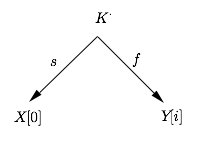
\includegraphics[width=1.5in]{images/p12.png} 
\end{figure}

Let $L$ be a soft truncation of $K^\cdot$ at degree $-i-1$ (note that $K$ is quism to $X[0]$ via $s$). It is easy to check

\begin{figure}[H] 
   \centering
   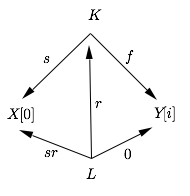
\includegraphics[width=1.5in]{images/p13.png} 
\end{figure}

commutes up to homotopy and $s,r$ are quisms. So in $\cD(\cA)$, we have $(s,f) \sim (sr,0)$ to $Y[i]$ for $i<0$. 

\item We have a relation to the Yoneda Extension: for $i \geq 0$, we look at the two definitions of $\Ext^i(X,Y)$. The ``classic" definition gives any exact sequence
\[
0 \ma{} Y \ma{} K^{-i+1} \ma{} \cdots \ma{} K^0 \ma{\ep} X \to 0
\]
Call this sequence $\hat{K}$. We have a roof

\begin{figure}[H] 
   \centering
   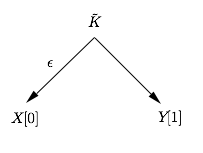
\includegraphics[width=1.5in]{images/p14.png} 
\end{figure}

i.e. an element of $\Ext_{\cA}^i(X,Y)=\Hom_{\cD(\cA)}(X[0],Y[i])$. It turns out to be all such elements of $\Ext_{\cA}^i(X,Y)$.


\item Let $I=$ the full subcategory of $\cA$ of injective modules. Consider $\cK^+(I)$, complexes bounded below, of injective objects with morphisms being composition. Then the obvious functor $\cK^+(I) \to \cD^+(\cA)$ is an equivalence of categories. This is proven on 179-183 of GM. We have a similar statement for the category of projectives $\cK^-(P) \to \cD^{-}(\cA)$. In the proof, one also gets if $X \in \chh^-(P)$ or $Y \in \chh^{-}(I)$, then $\Hom_{\cK(\cA)}(X,Y) \cong \Hom_{\cD(\cA)}(X,Y)$ as sets. The reveres direction here is exciting. It was first used to define $\Ext$ if the first component projective or second injective we are able to compute it. This gives a computation of $\Ext$ for objects $X,Y \in \cA$. So we have a new definition
\[
\begin{split}
\Ext_{\cA}^i(X,A) &\defeq \Hom_{\cD(\cA)}(X[0],Y[i]) \\
&=\Hom_{\cD(\cA)}(\dt{P},Y[i]) \\
&=\Hom_{\cK(\cA)}(\dt{P},Y[i]) \\
&=\Hom_{\chh(\cA)}(\dt{P},Y[i])/\text{homotopy}
\end{split}
\]

\item We have derived functors of $F$, $RF,LF$. See III.6 of GM. These are similar to $\Ext,\Tor$ and the class $L_nF$ and $R_nF$ but don't take homology. $R\Hom(X,Y) \defeq \Hom(\dt{P},Y)$ as a complex in $\chh(\cA)$ or $\cK(\cA)$ or $\cD(\cA)$ which are nicer to work with then $H^i$. 

\end{enumerate}
\end{rem}




% !TEX root = ../../homo_alg.tex

\newpage
\section{Triangulated Categories}

\subsection{Distinguished Triangles}

We now formalize the property that we saw for $\cK(A)$ and $\cD(A)$. Let $\tau$ be an additive category. Fix an additive automorphism $T: \tau \to \tau$, called the translate, translation, shift, or suspension of $\tau$. We write $X[1]=T(X)$ and $X[n]=T^n(X)$ for $n \in \Z$. A triangle is a triple of morphisms $(u,v,w)$ or $X \ma{u} Y \ma{v} Z \ma{w} \ma X[1]$ and a morphism of triangles is a commutative diagram
\[
\begin{tikzcd}
X \arrow{r} \arrow{d}{f} & Y \arrow{r} \arrow{d}{g} & Z \arrow{r} \arrow{d}{h} & X[1] \arrow{d}{f[1]} \\
X' \arrow{r} & Y' \arrow{r} & Z' \arrow{r} & X'[1]
\end{tikzcd}
\]
\begin{dfn}[Triangulated Category]
A triangulated category is an additive category $\tau$ with 
\begin{itemize}
\item translation
\item a collection of ``distinguished" triangles
\end{itemize}
such that 
\begin{enumerate}[(i)]
\item TR1a: $X \ma{1} X \ma{} 0 \ma{} X[1]$ is a distinguished triangle. 
\item TR1b: Any triangle which is isomorphic to a distinguished triangle is distinguished. 
\item TR1c: Any morphism $X \ma{u} Y$ can be completed to a distinguished triangle $(u,v,w)$, not necessarily uniquely. [However, the axioms for a triangulated category force this triangle to be unique.]
\item TR2: If $(u,v,w)$ is a distinguished triangle then its rotates $(v,w,-u[1])$ and $(-w[-1],u,v)$ are distinguished triangles.
\item TR3 (Completion of Morphisms): Given distinguished triangles given below and morphisms $f,g$
\[
\begin{tikzcd}
X \arrow{r} \arrow{d}{f} & Y \arrow{r} \arrow{d}{g} & Z \arrow{r} \arrow[dotted]{d}{h} & X[1] \arrow{d}{f[1]} \\
X' \arrow{r} & Y' \arrow{r} & Z' \arrow{r} & X'[1]
\end{tikzcd}
\]
such that the squares commute, there is a map $h: Z \to Z'$ completing the diagram to a map of triangles. Note that $h$ is not necessarily unique. 
\item TR4 (Octahedral Axiom): Given morphisms $A \ma{u} B$, $B \ma{v} C$, and distinguished triangles $A \ma{u} B \ma{j} C' \ma{\beta} A[1]$, $B \ma{v} C \ma{x} A' \ma{i} B[1]$, and $A \ma{vu} C \ma{y} B' \ma{\gamma} A[1]$, there is a distinguished triangle $(f,g,j[1] \circ i)$: $C' \ma{f} B' \ma{g} A' \ma{j[1] \circ i} C'[1]$ such that the following diagram commutes
\[
\begin{tikzcd}
C' \arrow[bend right=50,swap]{ddrr}{\exists f} \arrow[swap]{dr}{\beta} & & B \arrow[swap]{ll}{j} \arrow{dr}{v} & & A' \arrow[swap]{ll}{i} \arrow[bend right=40,swap]{llll}{j[1]i} \\
 & A \arrow{ur}{u} \arrow{rr}{vu} &  & C \arrow[swap]{ur}{x} \arrow{dl}{y} &  \\
 & & B' \arrow{ul}{\gamma} \arrow[bend right=50,swap]{rruu}{\exists g} & &  \\
\end{tikzcd}
\]
\end{enumerate}
\end{dfn}

\begin{rem}
Note that TR4 is often called the Octahedral Axiom as the commutative diagram is often given as
\[
\begin{tikzcd}
 \phantom{x} & B' \arrow[dotted]{dr}{g} \arrow[crossing over]{ddl}{\gamma} & \\
 C' \arrow{d}{\beta} \arrow[dotted]{ur}{f} & & A' \arrow{ll}{j[1]i} \arrow{ddl}{i} \\
 A\arrow{dr}{u} \arrow[crossing over]{rr}{vu} & & C \arrow{u}{x} \arrow[crossing over]{uul}{y} \\
 & B' \arrow{uul}{j} \arrow{ur}{v} & \\
\end{tikzcd}
\]
\end{rem}

The following proposition will show that the extension in TR1c is unique up to isomorphism and that in TR4, the octahedral maps $f,g$ are unique up to isomorphism of triangles. 

\begin{prop}
A distinguished triangle is determined up to isomorphism by any one of its maps. 
\end{prop}

Proof: This follows almost immediately from TR2 and TR3. \qed \\

\begin{prop}
In TR3, if $f,g$ are isomorphisms in $\tau$, then $h$ is an isomorphism in $\tau$.
\end{prop}

Proof: This follows similarly to the previous proof but makes use of the 5 Lemma for Triangles. \qed \\

\subsection{Cohomological Functors}

\begin{dfn}[Cohomological Functor]
An additive functor $H: \tau \to \cA$ from a triangulated triangle $\tau$ to an abelian category $\cA$ is called a cohomological functor if for any distinguished triangle $X \ma{u} Y \ma{v} Z \ma{w} X[1]$ the sequence $F(X) \ma{H(u)} F(Y) \ma{H(v)} F(Z) \ma{H(w)} F(X[1])$ is exact. 
\end{dfn}

\begin{ex}
There are two main examples of cohomological functors:
\begin{enumerate}[(i)]
\item The $0^\text{th}$ homology
\[
\begin{split}
H^0:& \cK(\cA) \to \cA \\
H^0:& \cD(\cA) \to \cA 
\end{split}
\]
where $X^0 \mapsto H^0(X^0)$. Note that $H^0(W[i])=H^i(W)$ for any complex $W$ in $\cK(\cA)$ and $\cD(\cA)$. 
\item In any triangulated category $\tau$, $\Hom_\tau(U,-)$ is a cohomological functor. 
\end{enumerate}
\end{ex}

\begin{lem}
Let $\tau$ be a triangulated category. Fix an object $U$ on $\tau$ then $\Hom_\tau(U,-)$ is a cohomological functor from the triangulated category $\tau$ to an abelian category. Similarly, $\Hom_\tau(-,U)$ is a functor from $\tau$ to an abelian category. 
\end{lem}

Proof: Consider $\Hom_\tau(U,0)$ -- the other direction is similar. It is enough to show that for any distinguished triangle $X \ma{u} Y \ma{v} Z \ma{w} X[1]$ that the sequence
\[
\Hom(U,X) \ma{u_*} \Hom(U,Y) \ma{v_*} \Hom(U,Z)
\]
is exact at $\Hom(U,Y)$ as the exactness for the rest of the sequence is obtained by translation, rotation, or shift by TR2. It is a simple exercise to see that $vu=0$ for any distinguished triangle. Applying $\Hom(U,-)$, we obtain $v_*u_*=0_*=0$ so $\im u_* \subset \ker v_*$. Conversely, let $f \in \ker v_*$ so that $v_*(f)=vf=0$. By TR1, we know that $U \ma{1} U \ma{} 0 \ma{} U[1]$ is a distinguished triangle. There is then a commutative diagram 
\[
\begin{tikzcd}
U \arrow{r}{1} \arrow[dotted]{d} & U \arrow{r}{0} \arrow{d}{f} & 0 \arrow{d} \arrow{r} & U[1] \\
X \arrow{r}{u} & Y \arrow{r}{v} & Z \arrow{r}{w} & X[1]
\end{tikzcd}
\]
Rotate, lift, rotate, to get a map of distinguished triangles, that is to obtain a map $U \ma{h} X$ such that $uh=f$. But $uh=u_*(h)$ so that $f \in \im u_*$. But then the sequence is exact. 

We now prove a previous proposition.

\begin{prop}
In TR3, if $f,g$ are isomorphisms in $\tau$, then $h$ is an isomorphism in $\tau$.
\end{prop}

Proof: Given the diagram in TR3
\[
\begin{tikzcd}
X \arrow{r} \arrow{d}{f} & Y \arrow{r} \arrow{d}{g} & Z \arrow{r} \arrow{d}{h} & X[1] \arrow{d}{f[1]} \\
X' \arrow{r} & Y' \arrow{r} & Z' \arrow{r} & X'[1]
\end{tikzcd}
\]
with $f,g$ isomorphisms, apply $\Hom_\tau(Z',-)$ (a cohomological functor) to get a commutative diagram with exact rows (by the previous lemma)
\[
\begin{tikzcd}
\Hom_\tau(Z',X) \arrow{r} \arrow{d}{f} & \Hom_\tau(Z',Y) \arrow{r} \arrow{d}{g} & \Hom_\tau(Z',Z) \arrow{r} \arrow{d}{h} & \Hom_\tau(Z',X[1]) \arrow{d}{f[1]} \\
\Hom_\tau(Z',X') \arrow{r} & \Hom_\tau(Z',Y') \arrow{r} & \Hom_\tau(Z',Z') \arrow{r} & \Hom_\tau(Z',X'[1])
\end{tikzcd}
\]
As $f,g$ are isomorphisms and the fact that translation is an automorphism, we know that $f[1]$ and $g[1]$ are isomorphisms. So $f_*,g_*,f[1]_*,$ and $g[1]_*$ are isomorphisms. Then by the 5 Lemma, we know that $h_*$ is an isomorphism. \qed \\

\subsection{The Cone in Triangulated Categories}

If $\tau$ is a triangulated category then we know that any morphism $X \ma{u} Y$ extends -- uniquely up to isomorphism -- to a distinguished triangle $X \ma{u} Y \ma{v} Z \ma{w} X[1]$. Then $Z$ with maps $v,w$ is called the cone of $u$, written $C(u)$. Note that in $\cD(\cA)$ and $\cK(\cA)$, $C(u)$ is actually the mapping cone of $u$.

\begin{thm}
Let $\cA$ be an abelian category. The category $\cK(\cA)$ with translation being shift [1] of complexes and distinguished triangles being those isomorphic (up to homotopy) to a triangle of the form $X \ma{u} Y \ma{} C(u) \ma{} X[1]$ is a triangulated category. Likewise, $\cK^+(\cA), \cK^-(\cA)$, and $\cK^b(\cA)$ are also triangulated categories. 
\end{thm}

Proof: We show this for $\cK(\cA)$ only. We need verify the axioms.
\begin{enumerate}[1]
\item The last parts of TR1 follow from the definitions and from the fact that $X \ma{u} Y \ma{} C(u) \ma{} X[1]$ is distinguished. The first part of TR1 follows from the fact that 
\[
\begin{tikzcd}
X \arrow{r}{1} \arrow{d}{1} & X \arrow{d}{1} \arrow{r} & 0 \arrow{r} \arrow{d} & X[1] \arrow{d}{1} \\
X \arrow{r}{1} & X \arrow{r} & C(1) \arrow{r} & X[1]
\end{tikzcd}
\]
One need check that the diagram commutes that that it is an isomorphism of triangles. The only real work in this step is in checking that $0 \to C(1)$ is homotopic to the identity of $C(1)=X[1] \oplus X$. The homotopy is
\[
1_{C(1)}= hd+dh, \text{ where, }h= \begin{pmatrix} 0 & 0 \\ 1_X & 0 \end{pmatrix}
\]
\item Let $X \ma{u} Y \ma{v} Z \ma{w} X[1]$ be a distinguished triangle. We need show that $Y \ma{v} Z \ma{w} X[1] \ma{-u[1]} Y[1]$ is a distinguished triangle (the converse can be proved by repeated translations). To see that the second triangle is distinguished, we give an isomorphism between it and the distinguished triangle $Y \ma{v} Z \ma{s} C(v) \ma{t} Y[1]$. As the triangle $X \ma{u} Y \ma{v} Z \ma{w} X[1]$ is distinguished, we can assume that $Z=C(v)=X[1] \oplus Y$, or else compose with the natural isomorphisms. Note that
\[
d_{C(v)}= \begin{pmatrix} -d_Y & 0 & 1_Y \\ 0 & -d_X & u[1] \\ 0 & 0 & d_Y \end{pmatrix}
\]
Define $\theta: X[1] \to C(v)$ by $\theta^i(x^{i+1})=(-u^{i+1}x^{i+1}, x^{i+1},0)$ for $x^{i+1} \in X[1]^i=X^{i+1}$. We have the diagram
\[
\begin{tikzcd}
Y \arrow{r}{v} \arrow{d}{1} & Z \arrow{d}{1} \arrow{r}{w} & X[1] \arrow{r}{-u[1]} \arrow{d}{0} & Y[1] \arrow{d}{1} \\
Y \arrow{r} & Z \arrow{r}{s} & C(v) \arrow{r}{t} & Y[1]
\end{tikzcd}
\]
We want to show that this diagram is a morphism of triangles in $\cK(\cA)$. It is easy to check this using the explicit formulas for $s,\theta w$ and that $h^i: Z^i \to C(v)^{i-1}$ given by $h^i(x^{i+1},y^i)=(y^i,0,0)$ is the necessary homotopy. One need also verify that this is an isomorphism of triangles but this was done earlier in a previous proof. 

\item To see TR3, given distinguished triangles $X \ma{u} Y \ma{} C(u) \ma{} X[1]$ and $X' \ma{u'} Y' \ma{} C(u') \ma{} X'[1]$ and maps $f: X \to X'$ and $g: Y \to Y'$, there is a map $h: C(u) \to C(u')$ given by $h\defeq g \oplus f[1]$. It is simple to check that $h$ is indeed a chain map. 

\item To see TR4, consider maps $A \ma{u} B$ and $B \ma{v} C$. We may assume that the distinguished triangles extending $u,v,$ and $vu$ are the standard ones with the cone in them. Otherwise, compose the result with the appropriate isomorphisms. Then we have
\[
\begin{tikzcd}
C(vu) \arrow{dr} \arrow[dotted,bend left=50]{rrrr}{g} & & C \arrow{ll} \arrow{rr} & & C(v) \arrow{dl} \arrow[bend left=50]{ddll}{(j[1] \circ i)[1]} \\
& A \arrow[swap]{rr}{u} \arrow{ur}{vu} & & B  \arrow{dl} \arrow[swap]{ul}{v} & \\
& & C(u) \arrow[dotted,bend left=50]{uull}{f} \arrow{ul} & & 
\end{tikzcd}
\]
We want to show that there exists $f,g$ so the outside ``loop" is a distinguished triangle. Define $f(b,a) \defeq (v(b),a)$ and $g(c,a) \defeq (c,u(a))$. One need check that $f,g$ are chain maps (maps of complexes): $fd=df$ and $gd=dg$ for differential $d$ and that the two new regions in the diagram commute: $\beta=\gamma f$ and $x=gy$ using the previous notation. 

Now to see that $C(u) \ma{f} C(vu) \ma{g} C(v) \ma{j[1]i} C(u)[1]$ is a distinguished triangle, note that $C(v)^n=C^n \oplus B^{n-1}$ and $C(f)=(C^n \oplus A^{n+1}) \oplus (B^{n-1} \oplus A^n$ and simply check that these ``work". Now if $\varphi$ is a homotopy equivalence, we have $\varphi: C(v) \to C(u(f))$ and $\psi: C(u(f)) \to C(v)$ where $\varphi(c,b)=(c,0,b,0)$ and $\psi(c,a,b,d)=(c,b)$. Check that $\varphi \psi \simeq 1$ and $\psi \varphi \simeq 1_{C(v)}$ and that $C(u) \ma{f} C(vu) \ma{g} C(v) \ma{j[1]i} C(u)[1]$ is the same as $C(u) \ma{f} C(vu) \ma{\varphi g} C(f) \ma{(j[1]i)\psi} C(u)[1]$ by showing the appropriate diagram commutes. To see that this last triangle is distinguished, one need check that $\varphi g$ is the normal inclusion and $(j[1]i)\psi$ is the usual projection (or homotopic to them). 
\end{enumerate}
\qed \\




\begin{thm}
Let $\tau$ be a triangulated category, e.g. $\cK(\cA)$, and $S$ a localizing class of morphisms. Suppose $S$ is compatible with the triangulation. That is, 
\begin{enumerate}[(a)]
\item $s \in S$ if and only if $T(s)=s[1] \in S$
\item In TR3, if $f,g \in S$ then $h$ can be chosen to be in $S$ as well 
\end{enumerate}
Then $S^{-1}\tau$ with data
\begin{enumerate}[(i)]
\item translation as before (for $\tau$) as $\text{obj }\tau=\text{obj }S^{-1}\tau$
\item distinguished triangles being those isomorphic to image of a distinguished triangle from $\tau$ under the functor $\tau \to S^{-1} \tau$ given by $x \mapsto x$ and $f \mapsto (1,f)$
\end{enumerate}
Then $S^{-1}\tau$ is a triangulated category. 
\end{thm}

Proof: The proof of this uses very careful tracking of roofs, see [GM] pp 251 - 256. \qed \\

\begin{cor}
The category $\cD(\cA), \cD^+(\cA), \cD^-(\cA),$ and $\cD^b(\cA)$ are triangulated. 
\end{cor}

Proof: Using the theorem, one only need check (a) and (b). But (a) is obvious and to see (b), let $S$ be the set of quasi isomorphisms. One cannot use the Triangulated Five Lemma as we do not know that $\cD(\cA)$ is triangulated. Instead, use the long exact sequence on homology from the two distinguished triangles. \qed \\





























% !TEX root = ../../homo_alg.tex

\newpage
\section{Spectral Sequences}
\subsection{Introduction}

Spectral sequences were developed by Leray for use in Algebraic Topology. During World War II, he was imprisoned by the Nazis. Not wanting them to know he was an applied mathematician, he stated he was a pure mathematician who worked in Algebraic Topology. During this time in the war, he developed spectral sequences. These were also independently developed by Lyndon in group cohomology. In 1945, Kozul made the procedure algebraic while in 1952 Massey created exact couples. 

We want to understand the homology of complexes: $H_n(\tot(C_{\cdot \cdot}))$. An example of this would be the calculation of Tor from homologies of individual columns/rows and the maps between them. More generally, $H_n(\dt{C})$, calculating the homology of a complex from parts (meaning subcomplexes and quotients) of it via factors in a filtration of $\dt{C}$ and maps between them. Spectral sequences provide an efficient machinery (more like bookkeeping) to paste these pieces together. 

For some motivation, take a double complex with two columns. 
\begin{figure}[h] 
   \centering
   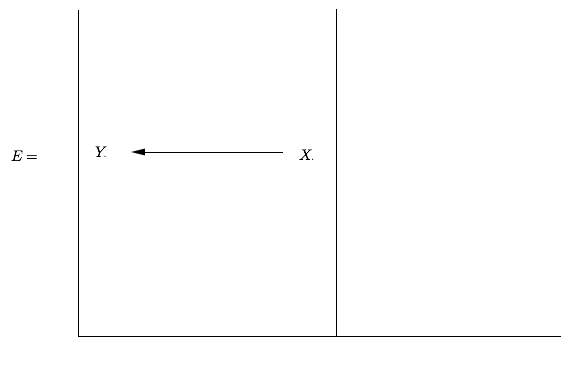
\includegraphics[width=4in]{images/ex1.png} 
\end{figure}

Then $\tot(E)$ is the mapping cone $C(f)$. From the short exact sequence
\[
0 \ma{} Y \ma{} C(f) \ma{} X[-1] \ma{} 0
\]
we get a long exact sequence 
\[
\cdots \ma{} H_{n+1}(X[-1]) \ma{\delta_{n-1}} H_n(Y) \ma{\beta} H_n(C(f)) \ma{\alpha} H_n(X[-1]) \ma{\delta_n} \ma{} \cdots
\]
where $\delta_{n+1}=H_n(f)$, $\delta_n=H_{n-1}(f)$, $H_n(X)=H_{n+1}(X[-1])$, $H_n(C(f))=H_n(\tot(E))$, and $H_{n-1}(X)=H_n(X[-1])$. So we get an exact sequence
\[
0 \ma{} \coker(H_n(f)) \ma{} H_n(\tot(E)) \ma{\alpha} \ker \delta \ma{} 0
\]
where $\ker \delta=\ker(H_{n-1}(f))=\im \text{ previous map}$ and $\coker H_n(Y)/\ker \beta=H_n(V)/\im H_n(f)$. That is, we get a filtration 
\[
H_n(\tot(E)) \supseteq \coker(H_n(f)) \supseteq 0
\]
where factoring yields $\ker(H_{n-1}(f))\cong H_n(\tot(E))/\coker(H_n(f))$ and $\coker(H_n(f)) \cong \coker(H_n(f))/0$. Notice the similarity between this and composition series. Another way to track the same data is to let $E_0=E$, called the $E^0$ or initial page, be given as above. In each position, take homology along the vertical direction to get the $E^1$ page
\[
\begin{tikzcd}
\phantom{x} & \vdots \arrow{d} & \vdots \arrow{d} & \\
0 & H_2(Y) \arrow{l} \arrow{d} & H_2(X) \arrow{l} \arrow{d} & 0 \arrow{l} \\
0 & H_1(Y) \arrow{l} \arrow{d} & H_1(X) \arrow{l} \arrow{d} & 0 \arrow{l} \\
0 & H_0(Y) \arrow{l} \arrow{d} & H_0(X) \arrow{l} \arrow{d} & 0 \arrow{l} \\
 & 0 & 0 & \\
\end{tikzcd}
\]
where the vertical maps are now 0, so they are no longer useful. However, the horizontal maps still carry useful information. So we take horizontal homology to get the $E^2$ page
\[
\begin{tikzcd}
\phantom{x} & \vdots \arrow{d} & \vdots \arrow{d} & \\
0 & \coker(H_2(f)) \arrow{l} \arrow{d} & \ker(H_2(f)) \arrow{l} \arrow{d} & 0 \arrow{l} \\
0 & \coker(H_1(f)) \arrow{l} \arrow{d} & \ker(H_1(f)) \arrow{l} \arrow{d} & 0 \arrow{l} \\
0 & \coker(H_0(f)) \arrow{l} \arrow{d} & \ker(H_0(f)) \arrow{l} \arrow{d} & 0 \arrow{l} \\
 & 0 & 0 & \\
\end{tikzcd}
\]
where now the horizontal maps are useful. However, we have maps along the diagonal (that is, along the lines $y= n-x$ for $n \in \Z \cup \{0\}$. But these turn out to be not useful. Taking homology along these diagonal lines changes nothing so we have
\[
E^2=E^3=E^4=\cdots=E^\infty
\]
Notice how we took the various maps
\begin{figure}[h] 
   \centering
   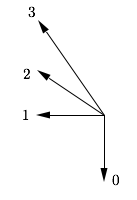
\includegraphics[width=1in]{images/maps.png} 
\end{figure}
Recall $H_n(\tot(E))$ has filtration with factors $\coker(H_n(f)), \ker H_{n-1}(f))$ which are in $E_2$ above (if we took $\tot$ with $p+q=n$, considering $(p,q)=(x,y)$). This is an interesting connection. 

As another example, take $E=E^0$ the bicomplex with differentials $d^V$ the vertical maps and $d^H$ the horizontal maps. To find $H_n(\tot(E))=Z_n/B_n$, we need to find the cycles. 
\begin{figure}[h] 
   \centering
   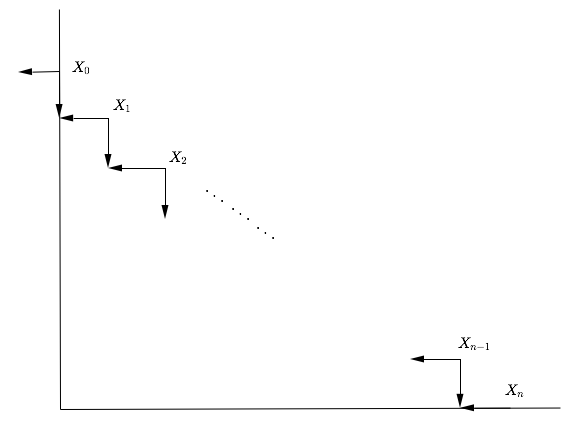
\includegraphics[width=3in]{images/diagonal.png} 
\end{figure}
That is, we want to find ordered tuples $x+y=n, i+j=n, p+q=n$, $\oplus_{p+q=n} E_{p,q}$ with $d^V(X_p)=d^H(X_{p+1})$ (so that they cancel out) and $d^H(X_0)=0$ and $d^V(X_n)=0$. But how do we do this? We start with $x_n \in \ker d^V$ so that $\overline{x_n} \in H_0(\text{column})$. Let $z_n=d^H(x_n)$. Now we have $Z_n=d^V(\text{some }x_{n-1})$ if and only if $z_n \in \im d^V$ if and only if $\overline{z}_n=0$ in $H_0(\text{column }n-1)$ if and only if $\overline{x}_n \in \ker(H_0(\text{column }n) \to H_0(\text{column }n-1)$. If so, we can assign to the $x_n$ the element $x_{n-1}$ and look at the $Z_{n-1}=d^H(X_{n-1})$, where the maps go between the $X_n$ two left and one up. Note throughout we have dropped $\pm$ on elements to make things work for simplification. That is, we take ``$\overline{x}_n \in H^H(H^V(\text{column}))$". So $E^1$ is the bicomplex with vertical homologies in $E^0$ and $E^2$ is the bicomplex with the horizontal homology of $E^1$. Continuing this process, one can see any element $\overline{x}_n$ surviving in spot $(p,q)=(n,0)$ on page $E^n$ can be represented by an $x_n$ that can be extended to give a cycle $(x_0,\cdots,x_n)$ in the original $H_n(\tot(E))$ with arrows $(r,0) \mapsto (r,r-1)$.

\subsection{Homology Spectral Sequence}

\begin{dfn}[(Homology) Spectral Sequence]
A (homology, so the arrows go down and left, that is not a cochain complex) spectral sequence in an abelian category $A$ is 
\begin{enumerate}[(i)]
\item a family of pages: $E^r=\{E_{p,q}^r\}$ of objects for all $p,q \in \Z$, $r \geq r_0$, i.e. the start page.
\item in each page, $E^r$ has maps $d^r: E_{p,q}^r \to E_{p-r,q+(r-1)}^r$ with $(d^r)^2=0$.
\item the objects in page $E^{r+1}$ satisfy $E^{r+1}_{p,q} \cong H_{p,q}(E^r,dr)$. That is, the homology of the previous page in each spot. 
\end{enumerate}
\end{dfn}

It is important to note that though we can draw $E^0$ in a grid with $d^0$, this does not have to be a bicomplex. Furthermore, note that $E^{r+1}_{p,q}$ is a sub quotient, i.e. a quotient of a submodule of $E^r_{p,q}$. So one might ask if the $E^{r+1}$ page inherits any properties from the $E^r$ page. This also shows that the $E$'s are only getting ``smaller". In fact, at any spot $(p,q)$ we have (via the Correspondence Theorem)
\[
0=B^{r_0}_{p,q} \subseteq \cdots \subseteq B^r_{p,q} \subseteq B^{r+1}_{p,q} \subseteq \cdots \subseteq Z_{p,q}^{r+1} \subseteq Z^r_{p,q} \subseteq \cdots \subseteq Z_{p,q}^{r_0} = E_{p,q}^r
\]
where the sequence of $B$'s are images of arrows lifted to $E_{p,q}^0$ with $B^r_{p,q}/Z_{p,q}^r \cong E_{p,q}^r$ in $E_0$.

\begin{dfn}
A spectral sequence is bounded if for each $n$, the ``$p+q=n$" diagonal has finitely many nonzero entries. 
\end{dfn}

Note that if a spectral sequence is bounded, the differentials $d^r$ coming in and out of each spot will eventually be zero maps. Why?
\[
E_{p+r,q-(r-1)}^r \ma{} E_{p,q}^r \ma{} E_{p-r,q+(r-1)}
\]
with sums $n+1,n,$ and $n-1$ respectively, will be 0 for large $n$. So $E^r_{p,q}=E_{p,q}^{r+1}=E_{p,q}^{r+2}=\cdots$. We call this minimal $r$ such that this occurs the stable value $E^\infty_{p,q}$. If the spectral sequence is not bounded, we have to do other things:
\[
E^\infty_{p,q} = \frac{\bigcap_r Z^r_{p,q}}{\bigcup_r B^r_{p,q}}
\]

\begin{dfn}
We say a spectral sequences converges to objects $\{H_n\}$ if for each $n$, the objects $\{E^\infty_{p,q} \;|\; p+q=n\}$ give factors in some filtration of $H_n$, written $E^{r_0}_{p,q} \to H_{p+q}$ or $E^{r_0}_{p,q} \to H_n$.
\end{dfn}

But this is useless unless $\{H_n\}$ is relevant to something about the original set-up used to make the spectral sequence, e.g. $E^0$ or something about the $E^0$ page. 

\subsection{Cohomology Spectral Sequence}

Now we define the dual version:

\begin{dfn}[(Cohomology) Spectral Sequence]
A (cohomology) spectral sequence is
\begin{enumerate}[(i)]
\item family of pages $E_r=\{E_r^{p,q}\}$ for all $p,q \in \Z$ and $r \geq r_0$
\item on each page, maps $d_r: E_r^{p,q} \to E_r^{p+q,q-(r-1)}$ with $(d_r)^2=0$.
\item $E_{r+1}^{p,q}=H_{p+q}(E_r^{p,q},d_r)$ (that is the homology of the previous page at the spot $p,q$).
\end{enumerate}
\end{dfn}

Note that if you reindex $E^{p,q}$ as $E_{p,-q}$ then this is the old definition of a homology spectral sequence. This shows that proving theorems for the homology spectral sequences shows them by a dual argument for the cohomology spectral sequence. 

\begin{dfn}
We say that $\{E_r^{p,q}\}$ is bounded if in each diagonal $p+q=n$, there are finitely many nonzero objects. If so, then eventually $E_r^{p,q}=E_{r+1}^{p,q}=\cdots$. We call this the stable value $E_\infty^{p,q}$. The spectral sequence converges to $\{H^n\}$ if for each $n$, objects in the diagonal $p+q=n$ are the factors in some filtration of $H^n$. We write $E_r^{p,q} \to H^{p+q}$ or $H^n$.
\end{dfn}

\begin{ex}
Any $\{E^{p,q}\}$ spectral sequence converges to $E^{p,q}_r \to \oplus_{p+q=n} E^\infty_{p,q} \defeq H_n$. That is,
\[
H^n \supseteq * \supseteq * \supseteq \cdots \supseteq 
\]
with factors $E_\infty^{s,n-s}$, $E_\infty^{p,n-p},\cdots, E^{\text{last}}_\infty$. We have a reversed conclusion for a cohomology spectral sequence. 
\end{ex}

\subsection{Filtrations and Bounded Spectral Sequences}

We have some ``inclusion" of spectral sequences:
\[
\text{General Spectral Sequence} \supseteq \text{Filtration Spectral Sequence} \supseteq \text{Spectral Sequence of a Double Complex}
\]
The Loray-Serre spectral sequence of a fibration is a type of filtration of a spectral sequence: if $F$ is a fiber ($\pi^{-1}(b)$ for some $b \in B$) and $B$ is the base
\[
F \ma{} E \ma{\pi} B
\]
We will see how from a complex $C$ with a filtration by subcomplexes to construct a spectral sequence from the homology of the factors converges to the homology of $C$. 

\begin{dfn}[Filtration]
A filtration of a chain complex $\dt{C}$ is a chain of subcomplexes 
\[
\cdots \subseteq F_{p-1}C \subseteq F_pC \subseteq \cdots \subseteq C
\]
\end{dfn}

We will assume that the filtration is bounded (any position in the complex eventually stabilizes for all $n$, i.e. there are only finitely many $(F_pC)_n \neq 0$) or bounded below or exhaustive:
\[
\bigcup_p F_pC = C
\]
Now we look at the construction of the filtration. 

\begin{figure}[h] 
   \centering
   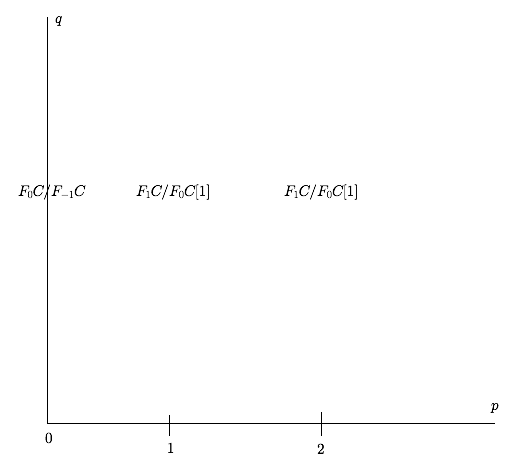
\includegraphics[width=4in]{images/grid.png} 
\end{figure}

Let $E^0_{p,q}=(F_pC/F_{p-1}C)_{p+q}=F_pC_{p+q}/F_{p+1}C_{p+q}$. That is, the $p$th column is the $p$th factor shifted down by $p$-steps. The differential $d$ on $C$ induces vertical maps (differential of factor complex $d^0: E^0_{p+q} \to E^0_{p,q-1}$). We know that $E^1_{p,q}=H_{p+q}(F_pC/F_{p-1}C)$. For the page $r$ (dropping the $p+q$ subscripts), let $\pi_p: F_pC \to F_pC/F_{p-1}C=E_p^0$ and $A^r_p=\{x \in F_pC \;|\; d(x) \in F_{p-r}C \}$, which are the ``cycles modulo $F_{p-r}C$". Then $Z_p^r=\pi(A_p^r) \supseteq B_p^r=\pi(d(A^{r-1}_{p+r-1}))$. We have $Z_p^r,B_p^r \subseteq F_pC/F_{p+1}C$. Note that we have
\[
0=B^0_p \subseteq B_p^1 \subseteq \cdots \subseteq B_p^r \subseteq \cdots \subseteq Z_p^r \subseteq \cdots \subseteq Z_p^1 \subseteq Z_p^0=E_p^0
\]
and let $E^r_p=Z^r/B_p^r \cong A^r_p/\left(d(A^{r-1}_{p+r-1})+A^{r-1}_{p-1}\right)$ (the congruence follows from the Second Isomorphism Theorem). Define $d^r$ to be the map induced by the original differential of $C$. One need check $(d^r)^2=0$ and $E^{r+1} \cong H(E^r,d^r)$. We have the following difficult (though not deep) Theorem:

\begin{thm}[Convergence Theorem]
If the filtration on $C$ is bounded or bounded below and exhaustive then the spectral sequence constructed above converges (this is trivial as it is bounded) to the homology of $C$: $E_{p,q}^1=H_{p+q}(F_p/F_{-1}) \to H_{p+q}(C)$. 
\end{thm}

We have the special case of the spectral sequence of a double complex. Then $\tot(C_{\cdot \cdot})$ has (at least) two canonical filtrations. The first is
\begin{figure}[h] 
   \centering
   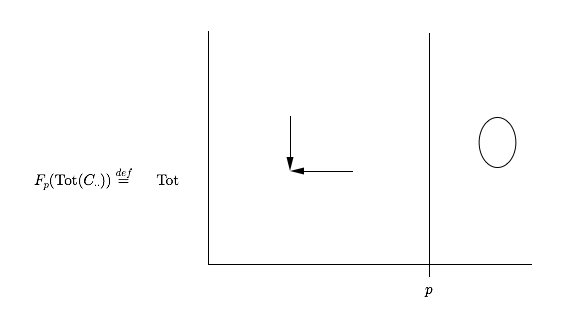
\includegraphics[width=4in]{images/almostfinal.png} 
\end{figure}
Note $E^0_{p,q} \defeq F_p/F_{p-1}= \text{column }p \text{ of } C_{\cdot \cdot}$ with $d^0$ the vertical differential $d^V$. We have $E^1_{p,q}=H^V_q(C_{p,*})$ and $d^1$ the differential induced by the original horizontal differential $d$ of $\tot(C_{\cdot \cdot})$ which is the horizontal differential induced by $d^H$ of $C_{\cdot \cdot}$ on the sub quotients (since $d^V(x)=0$ for all $\overline{x} \in H^V(C_{\cdot \cdot})$. So $E^2_{p,q}=H^H_pH^V_q(C)$. By the Convergence Theorem, we have $E^2_{p,q}=H^H H^V_q(C) \to H_{n=p+q}(\tot(C_{\cdot \cdot})$. The canonical construction follows similarly by exchanging the roles of $p,q$. 

\begin{figure}[h] 
   \centering
   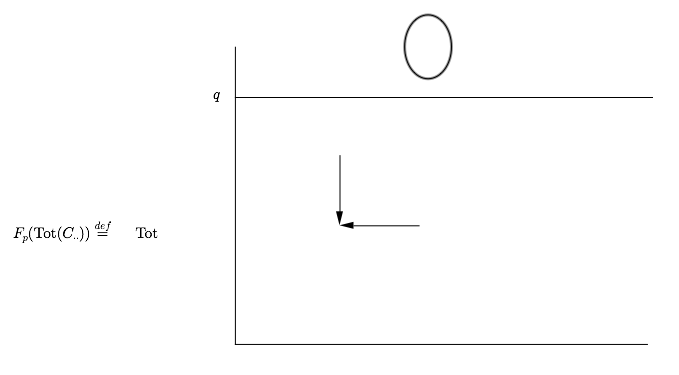
\includegraphics[width=4in]{images/final.png} 
\end{figure}

















































\end{document}